%% ----------------------------------------------------------------
%% Thesis.tex -- MAIN FILE (the one that you compile with LaTeX)
%% ---------------------------------------------------------------- 

% Set up the document
\documentclass[a4paper, 12pt, oneside]{Thesis}  % Use the "Thesis" style, based on the ECS Thesis style by Steve Gunn
\graphicspath{Figures/}  % Location of the graphics files (set up for graphics to be in PDF format)
\usepackage{verbatim}  % Needed for the "comment" environment to make LaTeX comments
\usepackage{vector}  % Allows "\bvec{}" and "\buvec{}" for "blackboard" style bold vectors in maths
\usepackage[pass]{geometry}
\usepackage{titlesec}
\usepackage[utf8]{inputenc}
\usepackage[english]{babel}
\usepackage[round, semicolon, authoryear]{natbib}
%\usepackage{apacite}
\bibliographystyle{apalike}
\usepackage{graphicx}
\usepackage{float}
\usepackage{bbm}
\usepackage{amsfonts}
\usepackage{tipa}
\usepackage[scientific-notation=true]{siunitx}
\usepackage{pdflscape}
\usepackage{afterpage}
\usepackage{xcolor}
\usepackage{tabularx}
\usepackage{capt-of}% or use the larger `caption` package
\usepackage[toc,page]{appendix}
\hypersetup{urlcolor=blue, colorlinks=true}  % Colours hyperlinks in blue, but this can be distracting if there are many links.
\usepackage[font=small,format=plain,labelfont=bf,textfont=normal,justification=justified,singlelinecheck=false]{caption}

%% ----------------------------------------------------------------
\begin{document}

\fontfamily{david}\selectfont
\frontmatter      % Begin Roman style (i, ii, iii, iv...) page numbering

% Set up the Title Page
\title{A computational study of phoneme representations and errors in reading}
\authors  {\texorpdfstring
            {\href{yair.lakretz@gmail.com}{Yair Lakretz}}
            {Yair Lakretz}
            }
\addresses  {\groupname\\\deptname\\\univname}  % Do not change this here, instead these must be set in the "Thesis.cls" file, please look through it instead
\date       {\today}
\subject    {}
\keywords   {}

\maketitle
%% ----------------------------------------------------------------

\setstretch{1.5}  % It is better to have smaller font and larger line spacing than the other way round

% Define the page headers using the FancyHdr package and set up for one-sided printing
\fancyhead{}  % Clears all page headers and footers
\rhead{\thepage}  % Sets the right side header to show the page number
\lhead{}  % Clears the left side page header

\pagestyle{fancy}  % Finally, use the "fancy" page style to implement the FancyHdr headers

%% ----------------------------------------------------------------
% Declaration Page required for the Thesis, your institution may give you a different text to place here
%\Declaration{

%\addtocontents{toc}{\vspace{1em}}  % Add a gap in the Contents, for aesthetics

%I declare that this thesis and the work presented in it are my own. I confirm that:

%\begin{itemize} 
%\item[\tiny{$\blacksquare$}] This work was done wholly or mainly while in candidature for a research degree at this University.
 
%\item[\tiny{$\blacksquare$}] Where any part of this thesis has previously been submitted for a degree or any other qualification at this University or any other institution, this has been clearly stated.
 
%\item[\tiny{$\blacksquare$}] Where I have consulted the published work of others, this is always clearly attributed.
 
%\item[\tiny{$\blacksquare$}] Where I have quoted from the work of others, the source is always given. With the exception of such quotations, this thesis is entirely my own work.
 
%\item[\tiny{$\blacksquare$}] I have acknowledged all main sources of help.
 
%\item[\tiny{$\blacksquare$}] Where the thesis is based on work done by myself jointly with others, I have made clear exactly what was done by others and what I have contributed myself.
%\\
%\end{itemize}
 
 
%Signed:\\
%\rule[1em]{25em}{0.5pt}  % This prints a line for the signature
 
%Date:\\
%\rule[1em]{25em}{0.5pt}  % This prints a line to write the date
%}
%\clearpage  % Declaration ended, now start a new page

%% ----------------------------------------------------------------
% The "Funny Quote Page"
%\pagestyle{empty}  % No headers or footers for the following pages

%\null\vfill
% Now comes the "Funny Quote", written in italics
%\textit{``''}

%\begin{flushright}
%If the quote is taken from someone, their name goes here
%\end{flushright}

%\vfill\vfill\vfill\vfill\vfill\vfill\null
%\clearpage  % Funny Quote page ended, start a new page
%% ----------------------------------------------------------------
% The Abstract Page
%\addtotoc{Abstract}  % Add the "Abstract" page entry to the Contents
%\abstract{
%\addtocontents{toc}{\vspace{1em}}  % Add a gap in the Contents, for aesthetics
%\begin{abstract}

Dyslexia is a common reading disorder, characterized by high rates of reading errors, and slow reading speeds, alongside normal intelligence. Research in the past decades has achieved major understandings about the processes involved in normal and abnormal reading, yet there is not one well accepted theory of dyslexia. Particularly, an ongoing debate remains on whether dyslexia is one central malfunction, as single-cause theories argue, or rather a general term describing multiple disorders, as the subtype approach to dyslexia argues. The latter view relies on the rich phenomenology of reading errors identified in research on dyslexia subtypes. For example, A dyslexic person may read the word {\it tries} as 'tiers', as 'dries', or as 'trial'. The first error may be a letter-transposition error, the second may be a voicing-substitution error (since the phonemes /t/ and /d/ differ by voicing), and the third may be a visual error made on the right side of the word - each error corresponding to a different subtype of dyslexia. Research on subtypes of dyslexia has recently required turning to more specific questions in the field: recent studies have identified new subtypes of dyslexia, characterized by mapping a letter to an erroneous phoneme that differs by a single phonological feature compared to the correct one, as in the above example about voicing substitution. These phonological feature-based subtypes of dyslexias were found to involve specific phonological features but not others. It therefore remains unclear why some phonological features are more prone to participate in such substitution errors than others. Introducing a novel approach, this thesis addresses these questions regarding the subtype approach to dyslexia from a new,  computational, perspective. Chapter 1 addresses the debate regarding the heterogeneity of dyslexia by exploring probabilistic graphical models to analyze patterns of reading errors made by dyslexic people. Results support a model assuming multiple dyslexia subtypes, that of a heterogeneous view of dyslexia. Moreover, the models achieve good diagnosis-prediction performance when compared to labels given by clinicians, thus providing the first automated diagnosis tool for dyslexia. The next two chapters address the question regarding the prevalence of phonological feature-based subtypes of dyslexia. Phonological feature-based errors may follow similarity relations among phonemes, assuming the more similar two phonemes are the more prone they are to confusion. Chapter 2 establishes a new approach to study phoneme similarity, which enables the quantification of the contribution of various phonological features to overall perceptual phoneme similarity, based on behavioral data. Different contributions of phonological features to phoneme similarity may explain the prevalence of specific feature-based dyslexia subtypes. Results show that for English, the voicing, nasality, distributed-strident and approximant features have the highest contribution to perceptual distances among phonemes. For Hebrew, a similar order among phonological features emerges, however, the voicing feature was found to be less perceptually discriminative compared to English. In both languages, it is shown that manner-of-articulation features dominate the similarity structure among phonemes. Departing from behavioral data, chapter 3 study the similarity structure among phonemes, based on neuronal data. In this chapter, we present and characterize data of single-cells activity recorded from high-level auditory regions, collected from six neurosurgical patients who performed a listening task with phoneme stimuli. Results show that manner-of-articulation features also dominate the functional organization of phonemes in high-level auditory regions, as revealed by spiking activity, similarly to the results from chapter 2. Directly comparing the similarity structure revealed by spiking activity and that from behavioral results from chapter 2, we find a moderate correlation between the two. Finally, drawing on the results, we discuss the signification of these findings with respect to speech perception - we argue that our results provide support to auditory theories, and are contrast to gestural theories of speech perception. In sum, in the center of this thesis and motivating the questions it addresses is the rich phenomenology of error types in dyslexia. The question of the heterogeneity of dyslexia, and that of the existence of specific feature-based subtypes, are hereby addressed. In common to both investigations, the thesis adopts a novel methodological approach to reading, which designs computational models to study these questions. This methodology has been hardly adopted to explore questions regarding reading and its disorders, this thesis therefore suggests new insights about persisting questions and debates in the field from yet unexplored perspective.

\end{abstract}
%}

%\clearpage  % Abstract ended, start a new page
%% ----------------------------------------------------------------

%\setstretch{1.3}  % Reset the line-spacing to 1.3 for body text (if it has changed)

% The Acknowledgements page, for thanking everyone
%\acknowledgements{
\addtocontents{toc}{\vspace{1em}}  % Add a gap in the Contents, for aesthetics

%\input{Chapters/acknowledgements.tex}

%}
\clearpage  % End of the Acknowledgements
%% ----------------------------------------------------------------

\pagestyle{fancy}  %The page style headers have been "empty" all this time, now use the "fancy" headers as defined before to bring them back


%% ----------------------------------------------------------------
\lhead{\emph{Contents}}  % Set the left side page header to "Contents"
\tableofcontents  % Write out the Table of Contents

%% ----------------------------------------------------------------
\lhead{\emph{List of Figures}}  % Set the left side page header to "List if Figures"
\listoffigures  % Write out the List of Figures

%% ----------------------------------------------------------------
\lhead{\emph{List of Tables}}  % Set the left side page header to "List of Tables"
\listoftables  % Write out the List of Tables

%% ----------------------------------------------------------------
\setstretch{1.5}  % Set the line spacing to 1.5, this makes the following tables easier to read
%\clearpage  % Start a new page
%\lhead{\emph{Abbreviations}}  % Set the left side page header to "Abbreviations"
%\listofsymbols{ll}  % Include a list of Abbreviations (a table of two columns)
%{
% \textbf{Acronym} & \textbf{W}hat (it) \textbf{S}tands \textbf{F}or \\
%\textbf{LAH} & \textbf{L}ist \textbf{A}bbreviations \textbf{H}ere \\

%}

%% ----------------------------------------------------------------
% End of the pre-able, contents and lists of things
% Begin the Dedication page

\setstretch{1.3}  % Return the line spacing back to 1.3

\pagestyle{empty}  % Page style needs to be empty for this page
%\dedicatory{For/Dedicated to/To my\ldots}

\addtocontents{toc}{\vspace{2em}}  % Add a gap in the Contents, for aesthetics


%% ----------------------------------------------------------------
\mainmatter	  % Begin normal, numeric (1,2,3...) page numbering
\pagestyle{fancy}  % Return the page headers back to the "fancy" style

%\titleformat
%{\chapter} % command
%[display] % shape
%{\bfseries\Large\itshape} % format
%{} % label
%{0.5ex} % sep
%{
%    \rule{\textwidth}{1pt}
%    \vspace{1ex}
%    \centering
%} % before-code
%[
%\vspace{-0.5ex}%
%\rule{\textwidth}{0.3pt}
%] % after-code
\titleformat{\chapter}[display]
{\normalfont%
    \tiny% %change this size to your needs for the first line
    \bfseries}{}{20pt}{%
    \LARGE %change this size to your needs for the second line
    }


%% General Introduction
\lhead{\emph{General Introduction}}
\chapter*{General Introduction}
\addcontentsline{toc}{chapter}{General Introduction}
\begin{figure}[H]
\vspace{.3in}
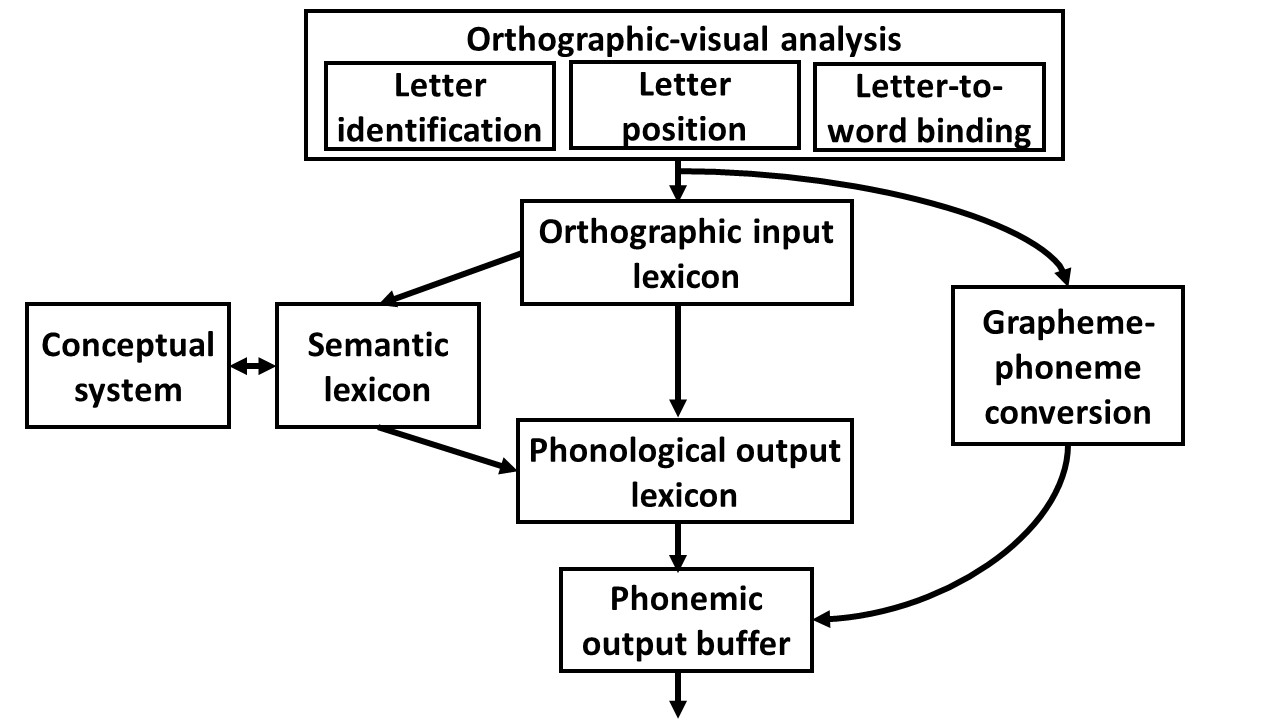
\includegraphics[width=\linewidth]{Figures/Ch1/DualRoute}
\caption{The dual-route model \citep{friedmann2016types})}
\end{figure}

\textit{Reading and dyslexia - rich phenomena, open questions}

Reading and dyslexia - rich phenomena, open questions
Reading is a complex and unique skill of the human brain. Reading aloud requires the brain to perform multiple low and high level processes, such as graphical pattern recognition, composition of letters into words, grapheme-to-phoneme conversion, phoneme production and, regularly, ascription of meaning – all almost in parallel and in strikingly short time and accuracy. Reading is thus a fertile ground for studying many processes that take place in the brain. Much can be learned about our visual, auditory, and motor systems, and their interactions, from the understanding of reading processes.

Research on reading focuses on both normal and abnormal reading. The study of abnormal reading, such as in the case of dyslexia, has been highly contributional to the theoretical understanding of the process of reading itself, as well as for clinical purposes. Understandings about the processes underlying normal reading were often derived from the analysis of data such as reading errors \citep{mn73, ck12}, reaction times \citep{s98, s00} and eye movements \citep{jainta2011dyslexic}, during reading of dyslexic people. Similarly, in neuroscience, studies of reading have explored brain activity of both normal and dyslexic subjects \citep{gaab2007neural, shaywitz2002disruption, price2012review}.

To this day, research on reading and dyslexia has reached major understandings, suggesting general cognitive theories \cite{stanovich1988explaining, vellutino1995semantic, ramus2003relationship, amitay2003reply, ck12}, characterization of the neuronal activity involved in the process \citep{joubert2004neural, gaab2007neural, dehaene2010children}, and possible clinical interventions \citep{coltheart1989treatment, aylward2003instructional, kipp2008remediation}. However, to this day, there is no consensus on one theory of reading and dyslexia. In fact, the term 'dyslexia' has received a multitude of definitions and descriptions in the literature, and various theories have been proposed to account for related behavioral findings, and have suggested various underlying causes of dyslexia \citep{eg14}. This fact also impacts the interpretation of results from neuroscience, as the definition of the deficit of subjects participating in the experiments depends on the theoretical school you ask. 

Accepted theories of dyslexia today span from single-cause \citep{stanovich1988explaining, s98, s00} and dual-cause \citep{wolf1999double}, to multifactorial-cause theories \citep{ck12}. The single-cause theory proposes that dyslexia is caused by a general phonological deficit and may be assessed by measuring reading accuracy and reaction time. The multifactorial-cause theory proposes to discern the term dyslexia into various subtypes with different causes, each characterized by making a specific type of errors. As oppose to single-cause theories, the subtype approach to dyslexia analyze the types of errors made by dyslexia people. For example, the word 'leaf' can be read as 'lead', as 'leave', or as 'laugh', and the word 'bear' can be read as 'bean', as 'pear', or as 'bare'. The first type of error in all cases can be characterized as consonant substitution, the second as voicing substitution (since both phoneme pairs /f/-/v/ and /b/-/p/ differ by the voicing feature), and the third as vowel substitution. According to this theory, specific types of errors point to specific sub-processes in normal reading, which are selectively impaired in different subtypes of dyslexia. In sum, whether dyslexia has a single cause or should be discerned into subtypes remains a controversial issue in the field.

Joining this wider theoretical question, other more specific questions remain in the field. In particular, with regards to the subtype approach to dyslexia, questions remain regarding specific subtypes of dyslexia, as described in the following, after a short background on the subtype approach: The first researchers to distinguish different subtypes of dyslexia, and the first to propose a cognitive model of reading, which accounts for these different subtypes were \citet{mn73}. The model proposed was a Dual-Route model, in which reading takes place in two routes, activated in parallel upon reading. One route, the lexical route, serves for reading already known words, and is characterized by fast retrieval of words from long-term memory lexicons. The second route, the sub-lexical route, serves for reading new, non-familiar words, and is characterized by step-by-step conversion of graphemes to phonemes. In this model, each subtype of dyslexia, associated with specific error types, was to be explained by a malfunction of a specific locus in the model. With time, the discovery of new characteristic error types, that is, new subtypes of dyslexia, led to the modification and refining of the reading model. Figure 1 describes the most accepted version of the Dual-Route Model. 

With regards to the sub-lexical route, a general malfunction identified several decades ago, is called Phonological Dyslexia (for review, see \citealp{c96}). Individuals with this type of dyslexia can read words with which they are already familiar (words that exist in their orthographic input lexicon – Figure 1), but they make errors in reading non-familiar words. The hypothesized cause for these errors is a general malfunction related to the conversion of graphemes into phonemes. Recently, more specific subtypes of dyslexia of the sub-lexical route were reported, all characterized by malfunctions related to specific phonological features: \citet{Gvion2010} reported a person with selective conversion impairment reading ‘goat’ as ‘coat’ and ‘pear’ as ‘bear’ thus having voicing substitution errors. They therefore coined this subtype of dyslexia as ‘Dyslegzia’. \citet{Gvion2012} reported  a case in which only the nasality feature was affected (alongside the voicing feature), naming this dyslexia as 'Nasalexia'. Last, \citet{kf11} reported a new sub-lexical route dyslexia, in which only vowels are affected and not consonants, called, Vowel Letter Dyslexia. They reported 25 cases of individuals making errors of migrations, substitutions, omissions, or additions of a vowel letter, and showed, as for all the above subtypes of dyslexia, converging evidence that the impairment was located in the sub-lexical route and not in a different locus of the Dual-Route reading model. These phoneme-related subtypes of dyslexia - dyslegzia, nasalxia, and vowel-letter dyslexia - show impairments with respect to specific phonological features - voicing, nasality and vowels, correspondingly (recent evidences of substitutions among strident phonemes were also observed \citealp[unpublished]{friedmann}). However, there are are no known subtypes of dyslexia that specifically affect other phonological features. For example, there is no evidence for a deficit that generates phoneme substitutions related to the [labial] feature. It is currently unclear as to why some phoneme-related errors are more common in reading than others, and what is the underlying phonological structure that causes this discrimination. These sorts of questions and their research may now have an important contribution to the detailed understanding of reading, as the current scientific goal is to characterize the exact building blocks of these intricate processes.

In the center of this thesis and motivating the questions it addresses is the rich phenomenology of error types in dyslexia . The question of the heterogeneity of dyslexia, and that of the existence of specific phoneme-related subtypes, are hereby addressed. In common to both investigations, the thesis adopts a novel methodological approach to reading, which designs data-driven computational models to study these questions. The field of data-driven models has gone through a recent rapid growth and development in various scientific fields, but was hardly adopted to explore questions regarding reading and its disorders. As described below, this methodology may provide new insights about persisting questions and debates in the field.

\textit{Computational data driven models - a novel approach to reading}

With the advance in computing technologies, computational models of cognitive functions have widely spread in research, and so have computational models of reading become an acknowledged approach for investigating  reading and its disorders. Computational models enjoy several advantages over traditional theories, which complement box-and-arrows models as that of the Dual-Route model. First, they propose detailed simulations of normal human performance and allow the introduction of lesions into the simulations, which can then be compared to behavioral data collected from neuropsychological patients. Second, computational models are considered to be highly explicit, as they need to be specific about various implementational details, such as characteristic processing times and dynamics of their units. Finally, they propose falsifiable predictions, which are quantitative compared to those of verbal theories. These have  made computational models highly influential on the field.

In the field of computational modelling, a family of computational models which possesses its own unique advantages, is that of data-driven models. Data-driven models are based on learning algorithms, and are typically trained on large corpii of data from which they can extract various types of information. They usually require a relatively small number of prior assumptions about the process in question, and are therefore occasionally described under the slogan of: 'letting the data to speak for itself'. As a scientific approach, the data-driven approach is contrasted to the traditional hypothesis-driven one, and was suggested by some researches as an essetntial component in scientific research \citep{kell2004here}. Data-driven models have had tremendous success and have rapidly spread in other fields \citep{bell2009beyond, leonelli2014difference, lecun2015deep}. However, to this day, they have received minimal attention in the field of reading disorders. With the accumulation of data on reading, it seems that applying a data-driven approach to yet existing research questions in the field, may reach novel insights and may open new research paths.

\textit{A data driven approach to the study of reading and dyslexia - current study}

This thesis addresses open questions in the field of reading disorders through the construction of data-driven computational models. To address the question regarding the heterogeneity of dyslexia, chapter 1 presents data-driven models to the problem, which are trained on a large corpus of reading-error data. By this, it proposes a new approach to the persisting debate by letting the data "to speak for itself". More specifically, this chapter explores the generation process of reading-errors with probabilistic graphical models, making use of probability language to capture the complex generation process of reading errors. The learning algorithms used to train the models can discover possible hidden patterns in the data, thus shedding light on the issue in question. In addition, the study develops an automatic diagnostic tool of subtypes of dyslexia, based on error types, which lays the groundwork for easily accessible, cheap and fast screening tests. 

To address the question regarding the existence of specific phoneme-related subtypes of dyslexia, chapters 2 presents data-driven models to the problem of phoneme similarity, as the answer to question about phoneme-related subtypes may lie in the similarity relations among phonemes. Phoneme-related reading errors may follow phoneme similarity, since phoneme that are more similar to each other may be more prone to participate in substitution errors. Various studies have suggested means to measure phoneme similarity \citep{NicelyMiller1955} or compute it from subphonemic features (e.g., \citealp{Pierrehumbert1993}). However, given a theory of phonological features, it is unclear what is the contribution of each feature to the overall similarity. A difference with respect to some phonological features may make a pair of phonemes more perceptually distinguishable compared to differences in other features. For example, a difference with respect to nasality ([+nasal] vs. [-nasal]) as in /n/-/d/, may render the two more distinguishable compared to a difference with respect to, e.g., [labial] as in /n/-/m/. It thus seems crucial to quantify the contribution of various phonological features to the overall similarity. Finally, differences among features with respect to their perceptual saliency, may then explain differences in prevalence of phoneme-related subtypes of dyslexia. From a methodological point of view, this chapter differs from previous studies in phonology, which manually devised similarity functions (e.g., \citealp{Frisch1997}), by adopting a data-driven approach to the question of phoneme similarity.

Chapter 3 complements the inquiry into phoneme similarity from a neuroscientific point of view. It tests the dominance of various phonological features in neural representations of phonemes, as revealed from neural activity in auditory regions, using computational tools and data-driven models. In this chapter, we characterize spiking activity collected from single neurons in high-level auditory regions in the superior temporal gyrus, while aurally presenting consonant-vowel and vowel stimuli to neurosurgical patients implemented with deep electrodes. We then characterize the functional organization of phonemes from spiking activity, and quantify the dominance of various phonological features in the neural representations. Finally, we compare the neural representations and the perceptual similarities among phonemes from chapter 2. Taken together, these two chapters provide a characterization of both neural and cognitive similarity structures among phonemes.

%% Chapter 1
\lhead{\emph{Chapter 1: Probabilistic Graphical Models of Dyslexia}}
%\begin{abstract}
%Reading is a complex cognitive process, errors in which may assume diverse forms. In this study, introducing a novel approach, we use two families of probabilistic graphical models to analyze patterns of reading errors made by dyslexic people: an LDA-based model and two Na\"{\i}ve Bayes models which differ by their assumptions about the generation process of reading errors. The models are trained on a large corpus of reading errors. Results show that a Na\"{\i}ve Bayes model achieves highest accuracy compared to labels given by clinicians ($AUC = 0.801\pm0.05$), thus providing the first automated and objective diagnosis tool for dyslexia which is solely based on reading errors data. Results also show that the LDA-based model best captures patterns of reading errors and could therefore contribute to the understanding of dyslexia and to future improvement of the diagnostic procedure. Finally, we draw on our results to shed light on a theoretical debate about the definition and heterogeneity of dyslexia. Our results support a model assuming multiple dyslexia subtypes, that of a heterogeneous view of dyslexia.
%\end{abstract}

\chapter{Chapter 1: Probabilistic Graphical Models of Dyslexia}
\section{Introduction}
Reading is an intricate task involving multiple processes located in different areas in the brain \citep{price2012review}. Errors in reading can result from dyslexia, a disorder involving a variety of such errors. Dyslexia is a highly common disorder with estimates of prevalence ranging from 5\% to 17.5\% \citep{ss05}, pointing to the need for accurate and accessible diagnosis. However, current diagnostic procedures require experts, and are mostly lengthy and expensive. In this study, we aim to provide an accessible, reliable and cheap diagnosis tool for dyslexia. We do this by showing that rich probabilistic graphical models can diagnose dyslexia closely to how experts do, rendering them accurate, reliable and automated tool for diagnosis. Moreover, by providing probability distributions of errors given target words in screening tests, models can be used for future improvement of the diagnosis procedure and understanding of dyslexia. Finally, our results provide a novel and quantitative perspective on an ongoing debate regarding the nature of dyslexia (e.g., \citealp{eg14}).

A dyslexic person may read the word \textit{three} as \textit{there}, as \textit{tree} or as \textit{four}. Despite this heterogeneity, many studies in the field of reading disorders focus on measures of speed and accuracy to characterize dyslexia, thus possibly ignoring the rich structure of types of reading errors. These studies often assume a common phonological \citep{r14, rrddcw03, s98, s01} or sensorimotor \citep{s01} cause to all types of reading errors. However, an alternative approach views dyslexia as an umbrella term for various deficiencies, or dyslexia subtypes, each characterized by specific error types (e.g., \citealp{ck12, fc15, mn73}). According to this approach, each of the errors above could result from a different subtype of dyslexia. This approach suggests that fundamental aspects of reading disorders lay in the complex structure of reading errors.

We explore the structure of reading errors and the heterogeneity of dyslexia using probabilistic tools. Probabilistic graphical models have several advantages as a framework for modelling reading errors. Probabilistic models allow explicitly capturing a dependency structure among variables in the problem, making learning more efficient. Probabilistic graphical models provide both diagnoses and explicit error distributions per each type of dyslexia and target word, as learned from the corpus data, and can naturally follow an error-generation process.

We use two families of graphical models. First, we construct Na\"{\i}ve Bayes models which are well-known for having a good performance as classifiers with relatively low model complexity (see, e.g., \citealp{lit92}). These models are thus suitable for the classification of reading errors. Next, we construct a Latent Dirichlet Allocation based (LDA-based) model, which has been proven to well capture generation processes in the context of writing and text \citep{bnj03, rgss04}. In such a model, the generation of reading errors made by a dyslexic person is a more complex process than that in a Na\"{\i}ve Bayes model, as it assumes that errors are generated according to a mixture of subtypes of dyslexia. An LDA model is therefore a natural candidate for dyslexia analysis.

We compare the models on two different tasks. First, we identify the probabilistic model that best performs on the task of diagnosing dyslexia. We achieve this by comparing the diagnoses of the models to those of experts. Secondly, we explore which model best captures the complex structure of the patterns of reading errors. We achieve this by comparing the models on the task of predicting unseen errors. Finally, the performance of the models is used to explore the question of whether reading errors do result from different subtypes of dyslexia, or rather from one general malfunction.

The rest of the paper is organized as follows: section 1.2 describes the related literature of probabilistic graphical models and of dyslexia. It also provides a summary of the major views of dyslexia in the current literature of reading disorders. Section 1.3 describes the structure and size of the data that was used in this study. Section 1.4 provides a detailed description of the probabilistic graphical models. Finally, section 1.5 describes the results of this study: the performance of the models on the task of diagnosing dyslexia (section 1.5.1), and the performance of the models in predicting reading errors (section 1.5.2).


\section{Related work}
\subsection{Probabilistic graphical models}
The LDA model was introduced a decade ago to discover topics in documents, and has been most influential since. Three main algorithms for approximate inference in the model were proposed: Variational Expectation-Maximiz\-ation \citep{bnj03}, the Expectation-Propagation \citep{ml02}, and Collapsed Gibbs Sampling \citep{gs04}. In this paper we use the latter method. The generative process described by the LDA model commences in Dirichlet priors which are often chosen to be uniform. However, following the demonstration of the importance of using non-uniform priors for this model \citep{wmm09}, we use these and not uniform priors in this study.

\subsection{Dyslexia and reading errors}
Literature on reading disorders presents various accounts of the causes of developmental dyslexia. One central approach describes developmental dyslexia as a disorder that can be reduced into a single cause, and will be referred to hereby as the {\it single-type} approach. The most influential example of this approach is the {\it phonological deficit hypothesis}. According to this theory, developmental dyslexia originates from a deficit affecting either the representations and processing of speech sounds \citep{ss05, s00, s98}, or as other authors have argued, from the access to these representations \citep{rs08}. This hypothesis had influence on much research in neuroscience and brain imaging studies, e.g., \citep{bdvsgmg13, d09, vgpsh13, grggvfb02, r14, rrddcw03}.

Another central approach describes dyslexia as a heterogeneous disorder, having several different causes, and will be referred to hereby as the {\it subtypes} approach. The most influential example of this approach derives from the {\it Dual-Route Reading Model} \citep{cc93, ck12, mn73}, describing the process of reading by several processing stages and routes (General Introduction figure 1). According to this approach, there are subtypes of dyslexia, each resulting from a deficit or malfunction in a different stage in the process of reading. For example, reading {\it signs} as {\it sings} may result from a specific malfunction in letter position processing during the early visual-orthographic stage, and is in this case ascribed to Letter Position Dyslexia \citep{fg01}. However, reading {\it signs} while pronouncing the 'g', may be caused by Surface Dyslexia, characterized by reading irregular words according to the regular grapheme-to-phoneme conversion rules \citep{c83}. The deficit leading to Surface Dyslexia occurs in one of two long-term memory lexicons, the orthographic or phonological lexicon, or in the information processing between them. Brain imaging studies following this approach aim to identify the neural correlates of different subtypes of dyslexia, e.g., \citep{jct03, lptbadc09}.

The single-type approach and the subtypes approach use different procedures to diagnose dyslexia. The diagnostic procedure based on the single-type approach mainly uses phonological tasks, for example, asking the subject to swap between the first phonemes in the two words {\it fresh bread} (expecting to get {\it bresh fread}). When otherwise using reading tasks, the degree of dyslexia is assessed by measuring accuracy and speed in such tasks, while disregarding the types of errors which were made. However, the diagnostic procedure based on the subtypes approach mainly uses reading tasks, asking the subject to read aloud a list of words which are prone to erroneous reading. These tests assess the subtype of dyslexia by counting the errors made of each type. 

Another group of studies aim to characterize dyslexia subtypes (e.g., \citealp{p06}), however the diagnostic procedure in these studies is not based on data of error types in reading tests, but on measures of speed and accuracy in various tasks. Several such studies have proposed probabilistic models to analyze the data (e.g., \citealp{plljbrak12}). See also \citet{rp14} for analysis of reading aloud data, however in contrast to our study, they were not concerned with error types in reading tests but focused on reading of nonwords by normal subjects.

\section{The data}
We test our models on reading tests collected from 313 Hebrew-speaking individuals with developmental dyslexia, aged 7 to 62 years, all diagnosed in the Language and Brain laboratory in Tel-Aviv University. Out of the 313 subjects, 97 were diagnosed with an Attention Deficit Disorder (ADD) in addition to dyslexia. This is, to our knowledge, the largest reading-errors corpus used so far (see \citealp{p07, rbl14}). The battery of tests has two parts: (1) screening-tests: reading tests given for initial assessment of dyslexia (TILTAN battery, \citealp{fg03}), and (2) varying post-tests which are determined according to the results of the screening-tests. These are used to further specify the diagnosis. Since different subjects take different post-tests, only the corpus of the screening tests was used in this study.

The screening test is composed of 196 target words in Hebrew, which are prone to erroneous readings. The audio responses of subjects are recorded, and then encoded before used in the model. Responses were encoded by experts in dyslexia diagnosis and research, into one of 19 different error types (table 1.1). Each of the 313 subjects therefore read 196 words in the screening-test, resulting in a corpus consisting of a total of 61,348 pairs of target-word and response.

\begin{table}

\caption{List of error types and the possible responsible dyslexia types. NS - Normal State; LPD - Letter Position Dyslexia; VD - Visual Dyslexia; VLD - Vowel Letter Dyslexia; AD - Attentional Dyslexia; ND - Neglect Dyslexia; Other - Other types of dyslexia, such as phonological output buffer dyslexia or deep dyslexia, which are diagnosed based on additional post-tests.}

\centering
\begin{tabular}{|c|c|c|} \hline

& Error type & Dyslexia type\\
\hline
1 & Correct response & NS\\
2 & Consonant migration & LPD, VD\\
3 & Consonant omission & VD\\
4 & Consonant addition & VD\\
5 & Consonant substitution & VD\\
6 & Vowel migration & VLD, LPD, VD\\
7 & Vowel omission & VLD, VD\\
8 & Vowel addition & VLD, VD\\
9 & Vowel substitution & VLD, VD\\
10 & Semantic error & Other\\
11 & Morphological error & Other\\
12 & Surface error & SD\\
13 & Visual error (left side) & ND, VD\\
14 & Function word error & Other\\
15 & Letter doubling, or double omission & LPD, VD\\
16 & Attentional omission & AD\\
17 & Attentional vowel letter error & AD, VLD\\
18 & Attentional migration between words & AD\\
19 & Migration of end letters & VD\\

\hline\end{tabular}

%\balancecolumns
\bigskip
\end{table}

Based on the screening tests and on additional post-tests, had these been conducted, each subject is diagnosed by an expert by marking the subtypes of dyslexia that he or she has. We represent each diagnosis as a multi-label binary vector of length 7, corresponding to seven dyslexia subtypes: 'Letter position dyslexia', 'Attentional dyslexia', 'Neglexia', 'Surface dyslexia', 'Visual dyslexia', 'Vowel letter dyslexia' and 'Normal state'.

The collected data corpus is in Hebrew, therefore it is important to discuss the applicability of this work to other languages, specifically English. The underspecification of vowels in Hebrew makes the Hebrew orthography neighborhood denser than that of languages such as English. An example of this is that in Hebrew, letter transpositions inside a word are more likely to result in another existing word, than in English. This property makes some dyslexias more easily detectable in Hebrew than in English. However, once the relevant stimuli are selected for an English reading task, the same dyslexias with the same properties are detectable in both languages. And indeed, the dyslexias we describe have all been identified in English (For a comprehensive survey of this literature of dyslexia types in English, see for example \citealp{ck12}; for the specific dyslexias that we describe here see Letter position dyslexia: \citealp{ck12}; Attentional dyslexia: \citealp{sc98, sw77}; Neglexia: \citealp{vba10}; vowel dyslexia: \citealp{kf11}; Surface dyslexia: \citealp{bd95, cbc06, cc93, c83}). This work can therefore be expanded to English and other languages.  

\section{The Models}
Bayesian models are expressive statistical models. Typically, these are used for mathematically modeling assumptions regarding the manner in which data (in this case, reading errors), is generated. We construct three different probabilistic graphical models for this purpose: a Latent Dirichlet Allocation (LDA) model, and two Na\"{\i}ve Bayes models.

\vfill

\begin{figure*}
\vspace{.3in}
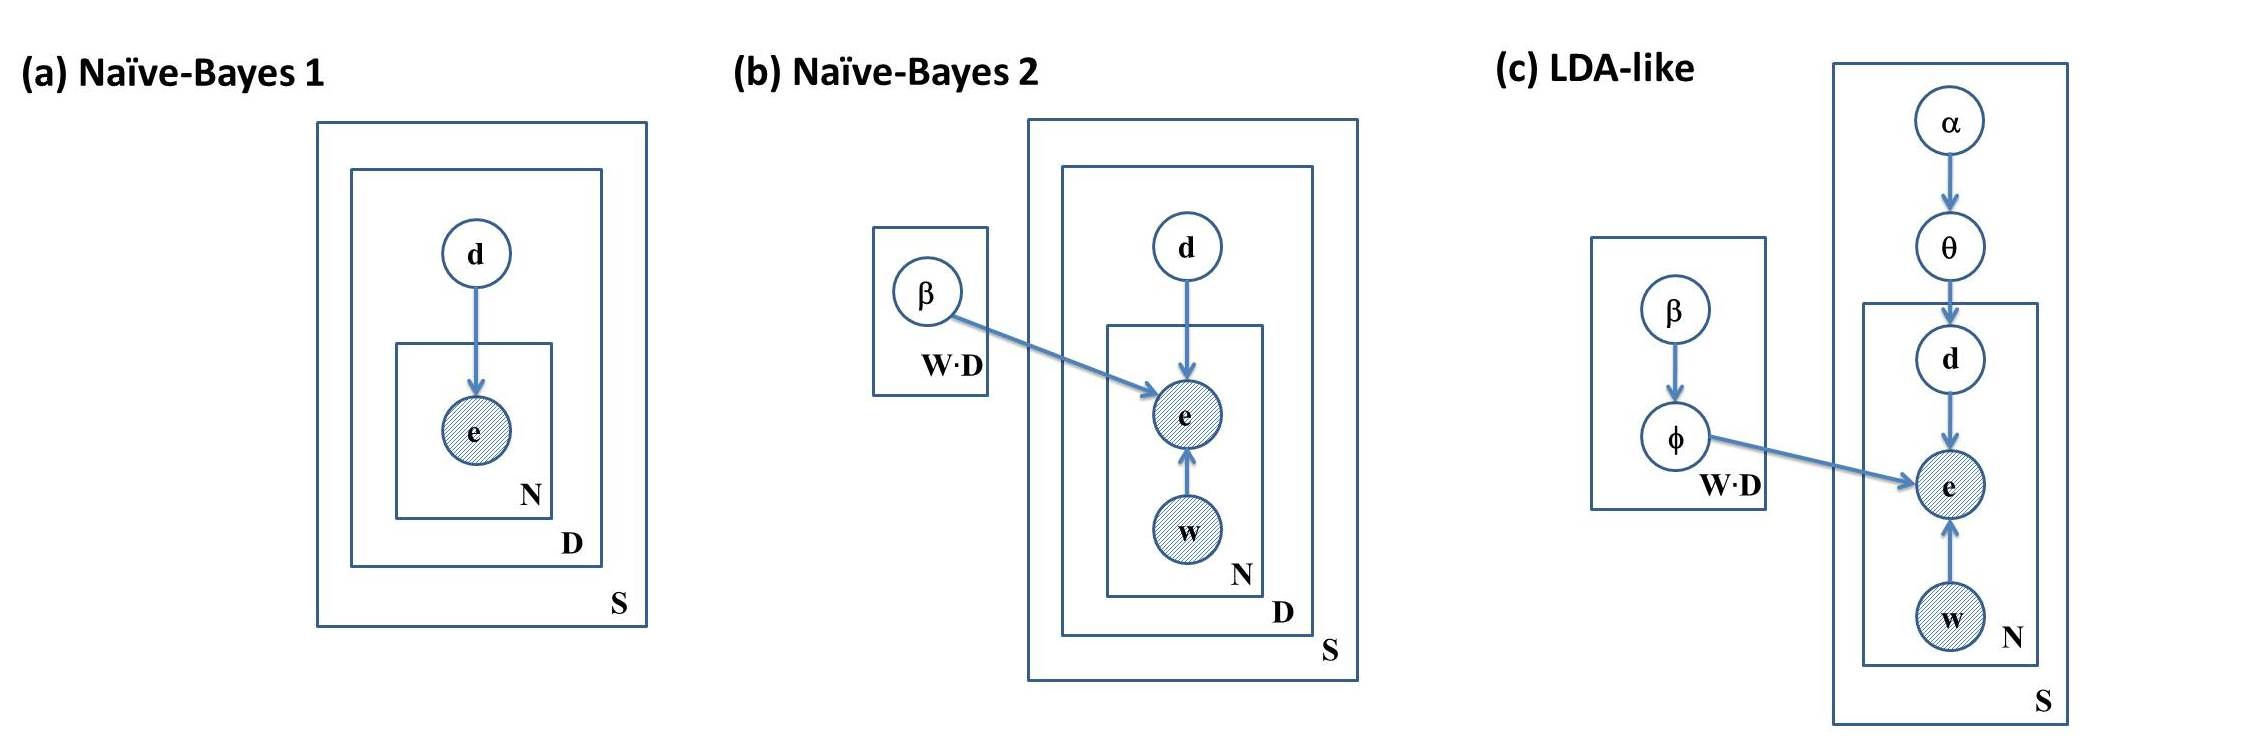
\includegraphics[width=\textwidth]{Figures/Ch1/figure_graphical_models}
\caption{Plate diagrams for all three models. (a) Na\"{\i}ve-Bayes 1 (b) Na\"{\i}ve-Bayes 2 (c) LDA-like model. $S$ represents the total number of subjects, $N$ the number of target-words in the screening test, $W$ the size of the vocabulary of the target-words, and $D$ represents the total number of dyslexia states. $e$ represents an error type, $w$ a target-word and $d$ a dyslexia state. In the LDA model, $\theta$ represents a diagnosis, $\phi$ represents a word-error-dyslexia distribution. $\alpha$ and $\beta$ are the Dirichlet priors for these distributions respectively.}
\end{figure*}

\subsection{Na\"{\i}ve Bayes models}
We begin to explore the generation process of reading errors with the class of Na\"{\i}ve Bayes models. Na\"{\i}ve Bayes models have shown much success in classification tasks, and could therefore fit the task of classifying reading error into dyslexia subtypes. 

The types of the errors made by the subjects are denoted in the models by $ e_i (i = 1, \dots , N) $. This variable takes one of $E$ possible values $ e_i \in {1, \dots , E} $, where $E$ stands for the number of possible error-types including a correct response. Another observed variable of the model represents the target-words. We denote it by $ w_i (i = 1, \dots , N) $, where $N$ represents the number of target-words in the screening-test. This variable can have one of $W$ possible values $ w_i \in {1, \dots , W} $. Since in our case each target-word is present only once in the screening-test, we have $ W = N $.

In all three models, a {\it dyslexia state} defines a hidden variable that stands for a state associated with a specific subtype of dyslexia, and is characterized by particular reading errors. For example, being in a state of low orthographic attention could be associated with Letter Position Dyslexia (LPD), typically leading to letter migration errors. We denote a dyslexia state by $d_i$, where $d_i$ can have one of D $ d_i \in {1, \dots ,D} $ dyslexia states. We have 7 such states as described above.

In all models, $S$ stands for the total number of subjects, $N$ stands for the number of target-words in the screening test, $W$ is the size of the vocabulary of the target-words, and $D$ stands for the total number of dyslexia states. $e$ represents an error type, $w$ a target-word and $d$ a dyslexia state.

\subsubsection{Word independent Na\"{\i}ve Bayes Model}
Typically, clinicians use the screening test to diagnose dys\-lexic subjects based on the total counts of different errors types they make. This approach disregards the specific target-words on which the errors were made, for instance, whether it is a word that many subjects misread, or specific subjects only. This diagnosis procedure can be modeled with a Na\"{\i}ve-Bayes model in which the probability of an error-type depends on the dyslexia subtype only. In what follows, we refer to this model as the Na\"{\i}ve Bayes 1 (NB1) model.

\paragraph{Model description}
For test results of a single subject, the joint distribution of the NB1 model factorizes as:
\[ p(\bar{e}, \bar{w}, d) = p(d) \prod_{i=1}^N p(e_i \mid d) p(w_i) \]
where the subscript $ i $ runs over all word-error pairs in the screening-test. Note that each error is independent of the specific target-word on which it was made. Figure 1.1a describes the plate diagram of the model.

\subsubsection{Word dependent Na\"{\i}ve Bayes Model}
A more complex model is a Na\"{\i}ve Bayes model in which the probability of an error is dependent on the dyslexia subtype and also on the target-word. We examine this model as well and will refer to it in what follows as the Na\"{\i}ve Bayes 2 (NB2) model.

\vfill

\paragraph{Model description}
In this model the response of the subject $ e_i $ is dependent on the $ i^{th} $ target-word $ w_i $ and on the dyslexia state $ d_i $. Similarly to the NB1 model, the joint distribution for the NB2 factorizes as:
\[ p(\bar{e}, \bar{w}, d ; \beta) = p(d) \prod_{i=1}^N p(e_i \mid d, w_i ; \beta) p(w_i) \]
where the subscript $i$ runs over all word-error pairs in the screening-test as before. Figure 1.1b describes the plate diagram of the model.

\subsection{The LDA model}
We continue our inquiry with a particular family of Bayesian models that has attracted much attention in the past decade, the Latent Dirichlet Allocation (LDA) Model \citep{bnj03}. The LDA model enables inferring unobserved variables given observed data, and has shown much success in capturing generative processes of text documents \citep{bnj03, rgss04}.

\subsubsection{Model description}
The LDA model captures the case where a person can suffer from a mixture of different dyslexia subtypes. According to this model, each person has a unique distribution over dyslexia subtypes. Additionally, each dys\-lexia subtype has a unique distribution of expected errors for a given target-word. When a person is reading a target-word, a particular dyslexia subtype is directing the way by which the word is read. The response is then dependent on this dyslexia subtype and the target-word. We therefore define two additional hidden variables. A {\it diagnosis} $ \theta_{s} $, which is a distribution over dyslexia states $ d_i $ for a subject. This distribution is learned from the data. A {\it word-error-dyslexia distribution} $ \phi_{wed} = p(e_i = e \mid w_i = w , d_i= d) $ is a distribution for all subjects in which, given a dyslexia state $d$ and a target-word $w$, each error has a certain probability of occurring. For example, given an LPD state, and the target-word {\it three}, the erroneous response {\it there} would be of high probability, but {\it tree} would be of a lower one. Similarly, given a normal state, and the target-word {\it three}, all error responses would have low probabilities except for the (correct) response {\it three}. 

The input to the model is the word-error pairs of all subjects. The hidden variables discovered by the model are: (1) $N$ dyslexia states for each subject; (2) the diagnosis of each subject - $ \theta_{s} $, and (3) a single word-error-dyslexia distribution $ \phi_{wed} $ for all subjects. Figure 1.1c describes the plate diagram of the dyslexia-state model.

\subsubsection{Dirichlet priors}
The generative process we use to model reading errors uses two Dirichlet priors from which the two distributions $ \theta_{s}$, $\phi_{wed} $ are sampled. Dirichlet priors are often chosen to be uniform. However, adding priors that adequately describe the generative process could enhance model performance. As the subtype approach to dyslexia has developed ways to detect typical reading errors for each dyslexia subtype, this prior knowledge can be incorporated into the LDA model. We tested the model both with this prior knowledge coded into it and without it.

The expert knowledge is used for sampling the word-error-dyslexia distribution and we denote it by $ \beta_{wed} $. This knowledge tells us about the error expected for each target-word given a dyslexia state (figure 1.1c). For example, given an LPD dyslexia-state, the word {\it three} is more likely to be read as {\it there} than {\it tree} or {\it four}. We incorporate this into the model by assigning a higher prior value $ \beta_{high} $ to the more probable responses of an LPD dyslexia-state, in this example {\it there}. We also assign a lower prior value $ \beta_{low} $ to the less probable responses, in this case {\it tree} and {\it four}. This is repeated for all dyslexia-states, including the normal state.

\vfill

\subsubsection{Parameter estimation}
Gibbs sampling is a form of a Markov Chain Monte Carlo (MCMC) method which is widely used for parameter estimation in topic models \citep{gs04, rgss04}. We use Gibbs sampling to construct a Markov chain between dyslexia-states, where the order of the Markov chain is based on the order of target-words in the reading-test. In each step, a dyslexia-state is sampled from its posterior distribution conditioned on all other variables in the model (see derivation below): 
\begin{equation}
\begin{split}
p(d_i = d\mid w_i = w, e_i = e, d_{-i}, w_{-i}, e_{-i}, \alpha, \beta) \propto \\
\frac{ C_{wed, -i} + \beta_{wed} } {\sum_{e'} [C_{we'd, -i} + \beta_{we'd}] } \frac{ C_{ds, -i} + \alpha_{ds} } {{\sum_{d'}[ C_{d's, -i} + \alpha_{d's}] }},
\end{split}
\end{equation}
where, $ d_i=d $ represents the assignment of the $ i^{th} $ word-error pair to dyslexia-state $d$. $ w_i = w $ represents the observation that the $i^{th}$ target-word is $w$, and $e_i = e $ represents the observation that the $i^{th}$ error type is $e$. $ d_{-i} $ represents all dyslexia-state assignments excluding the current $i^{th}$ instant. $ w_{-i} $ represents all target-words observations excluding the current $i^{th}$ instant. Similarly, $ e_{-i} $ represents all target-words observations excluding the current $i^{th}$ instant.
$ C_{wed, -i} $ represents the number of times the word-error pair ($w, e$) was assigned to the dyslexia-state $d$, excluding the current instance. $ C_{ds, -i} $ represents the number of times the dyslexia-state $d$ was assigned to the dyslexic person $s$. $ \alpha_{ds} , \beta_{wed} $ are the Dirichlet prior weights (see 4.1.2).
At each step of the Markov chain, we update the diagnoses of the subjects $ { \{ \theta_{s} \} }_{s=1}^S $ and the word-error-dyslexia distribution $ \phi_{wed} $ according to the dyslexia-state assignments $ \bar{d_{s}} $. These are then used to assess the accuracy and predictive power of the model.

We describe the derivation of the update rule (Eq. 1.1) following similar lines to those in \citet{gs04}, with the modifications required for our dyslexia-model (figure 1C):

The joint distribution of the model is given by:
\begin{equation*}
\begin{split}
&p(\bar{e},\bar{w},\bar{d},\Theta,\Phi;\alpha,\beta) = \\
&p(\Phi\mid\beta)p(\beta)\prod_{s = 1}^S p(\bar{e}_s\mid\bar{d}_s, \bar{w}_s) p(\bar{w}_s)p(\bar{d}_s\mid\Theta_s)\\ &p(\Theta_s\mid\alpha_s)p(\alpha_s) = \\
&p(\Phi\mid\beta) p(\beta) \prod_{s = 1}^S \prod_{i=1}^N p(e_{i, s} \mid w_{i, s}, d_{i, s}) p(d_{i, s}\mid\Theta_s) p(\Theta_s\mid\alpha_s)\\
&p(w_{i, s}) p(\alpha_s)
\end{split}
\end{equation*}
Given that $p(\Theta_s\mid\alpha_s)$ and $p(\Phi\mid\beta)$ are Dirichlet priors, and that $p(w_{i, s})$ are constant, rewriting the expression for the joint distribution, we get:
\begin{equation*}
\begin{split}
&p(\bar{e}, \bar{w}, \bar{d}, \Theta, \Phi; \alpha, \beta) \propto \\
&\prod_{s=1}^S \prod_{w=1}^W \prod_{e=1}^E \prod_{d = 1}^D \phi_{wed}^{C_{wed} + \beta_{wed} - 1} \theta_{ds}^{C_{ds} + \alpha_{ds} - 1}
\end{split}
\end{equation*}
Integrating out $\theta$ and $\phi$, we get:
\begin{equation*}
\begin{split}
&p(\bar{e},\bar{w},\bar{d};\alpha,\beta) \propto \\
&\iint \prod_{s=1}^S \prod_{w=1}^W \prod_{e=1}^E \prod_{d = 1}^D  \phi_{wed}^{C_{wed} + \beta_{wed} - 1} \theta_{ds}^{C_{ds} + \alpha_{ds} - 1} \mathrm{d}\theta \mathrm{d}\phi = \\
&\int \prod_{s=1} \theta_{ds}^{C_{ds} + \alpha_{ds} - 1} \mathrm{d}\theta \prod_{w=1}^W \prod_{d = 1}^D \int\prod_{e=1}^E \phi_{wed}^{C_{wed} + \beta_{wed} - 1} \mathrm{d}\phi = \\
&\frac{\prod_{d = 1}^D\Gamma(C_{ds} + \alpha_{ds})}{\Gamma(\sum_{d' = 1}^D (C_{d's} + \alpha_{d's}))}\prod_{w=1}^W\prod_{d = 1}^D \frac{\prod_{e = 1}^E\Gamma(C_{wed} + \beta_{wed})}{\Gamma(\sum_{e' = 1}^E (C_{we'd} + \beta_{we'd}))}
\end{split}
\end{equation*}
The posterior distribution for the $i^{th}$ dyslexic state can now be expressed using the expression for the joint distribution:
\begin{equation*}
\begin{split}
&p(d_i=d\mid w_i=w, e_i=e, d_{-i}, w_{-i}, e_{-i}; \alpha, \beta) \propto \\
&\frac{p(\bar{e},\bar{w},\bar{d};\alpha,\beta)}{p(\bar{e}_{-i},\bar{w}_{-i},\bar{d}_{-i};\alpha,\beta)}
\end{split}
\end{equation*}
The numerator and denominator of the above fraction, differ only by the counts having the $i^{th}$ pair of word-error in them, whereas all other terms cancel out. The posterior distribution thus results as the above update rule (Eq. 1.1).

\section{Experiments}
We conduct two experiments with the data. In the first, described in section 1.5.1, we compare three graphical models to find which model most accurately predicts dyslexia diagnosis. In principle, this model can be used to automate dyslexia diagnosis. In the second experiment, described in section 1.5.2, we compare the quality by which these three graphical models predict specific reading errors. The best model to predict errors could contribute to the better characterization of dyslexia.

\subsection{Experimental set-up}
We use two different types of cross validation, first leaving out a set of subjects and then leaving out a set of word readings of the test subjects. Specifically, we randomly split the data into a training-set with 219 subjects (70\%) and a test-set with 94 subjects (30\%), controlled to have the same proportion of subjects which are also diagnosed with Attention Deficit Disorder. See illustration in figure 1.2. The test-set is further divided into two equal-sized sets: a {\textit {\textbf {diagnosis-set}} with 98 pairs of target-words and subject responses, used to infer the diagnosis of test subjects, and a {\textit {\textbf {prediction-set}} also with 98 word-response pairs, used for assessing the predictions of the models. 

\begin{figure}[h]
\vspace{.3in}
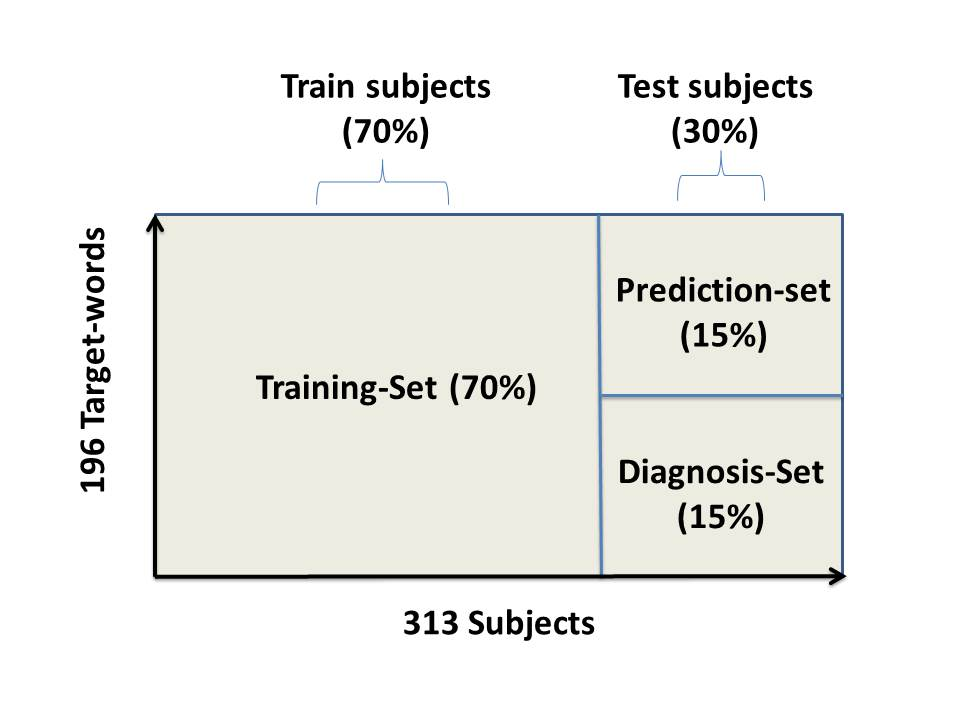
\includegraphics[width=\linewidth]{Figures/Ch1/trainTest2}
\caption{Data is partitioned into 3 sets. The dataset is first divided into a \textit {\textbf {training-set}} which contains reading-tests of 70\% of the subjects, and a test-set which contains the remaining 30\% of the data. The test-set is further divided into two subsets, a \textit {\textbf {diagnosis-set}} containing the first halves of the reading-tests, and a \textit {\textbf {prediction-set}} containing the remaining reading-tests of the test subjects.}
\end{figure}

\subsection{Probabilistic modeling as a dyslexia diagnosis tool}
Automation of the diagnosis process could facilitate the accessibility of the process to many people and increase awareness to treatment of specific reading deficits. We compare the automatic diagnosis of the three models -- NB1, NB2 and LDA -- to those given by experts, to test if the automated tool can indicate the diagnosed dyslexia type with high accordance to diagnoses given by experts.
We evaluate the diagnosis quality as follows. The automatic diagnosis is based on the diagnosis-set. This set is used to infer the diagnosis distribution $ \theta_{s} $ for each subject. The accuracy of the models is then assessed using the diagnoses given by experts. The prediction-set together with the diagnosis distribution $ \theta_{s} $ are later used for the evaluation of the predictive power of the models. The prediction-set is therefore not used in the diagnosis process.
Diagnosis quality of the two Na\"{\i}ve Bayes models, is estimated by computing 

\begin{equation}
p(d \mid \bar{e}) \propto p(d) \prod_{i = 1}^N [p(e_i \mid d)]^{C_{e_i}}
\end{equation}

\begin{equation}
p(d \mid \bar{e}, \bar{w}) \propto p(d) \prod_{i = 1}^N p(e_i \mid d, w_i)
\end{equation}

where the dyslexia prior $ p(d) $, the probability of error given a dyslexia subtype $ p(e_i |d) $, and the probability of an error given a dyslexia-type and a target-word $ p(e_i \mid d,w_i ) $ are evaluated from the training group.

For the LDA model, we train the model on the training-set together with the diagnosis-set. The model is initialized with random dyslexia state assignments $ { \{ \bar{d}_{s} \} }_{s=1}^P $ which are then iteratively sampled according to the sampling rule in $(1)$. At each step of this process, we update the dyslexia distribution per each subject $ \theta_{s} $ and the word-error-dyslexia distribution $ \phi_{wed} $ according to the new sampled dyslexia-state.

The reason we train the model on the training-set and the diagnosis-set together is to avoid a discrepancy between the hidden dyslexia-states of the word-error-dyslexia distribution $ \phi_{wed} $, learned from the training-set, and those of the dyslexia distributions $ { \{ \theta_{s} \} }_{s \in test-set} $, learned from the diagnosis set. If the model is trained on the sets separately, the hidden states of these distributions might differ by a permutation relation. All results below are averages over 5 splits of subjects to train- and test- sets (allocations of subjects), and also over 10 different random initializations of the dyslexia state assignments (a total of 50 runs). 500 iterations were found to suffice for convergence (figure 1.4A).

We compare the diagnoses given by the three models to those given by experts. The Na\"{\i}ve-Bayes models are known to be strong classifiers and were designed by similar assumptions and guidelines to the ones held by diagnosticians, and therefore their diagnoses are expected to strongly correlate with those given by experts. The LDA model is designed to capture the generative process of the patterns of reading errors, (see section 1.5.2) but may therefore be a worse predictor of dyslexia subtypes. 
Note also that the diagnoses of the clinicians are given according to the results of the entire screening-tests and the post-tests results, whereas the diagnoses of the models are based on only halves of the screening-tests. This is expected to lower the maximum accuracy for all models.

\begin{figure}[h]
\vspace{.3in}
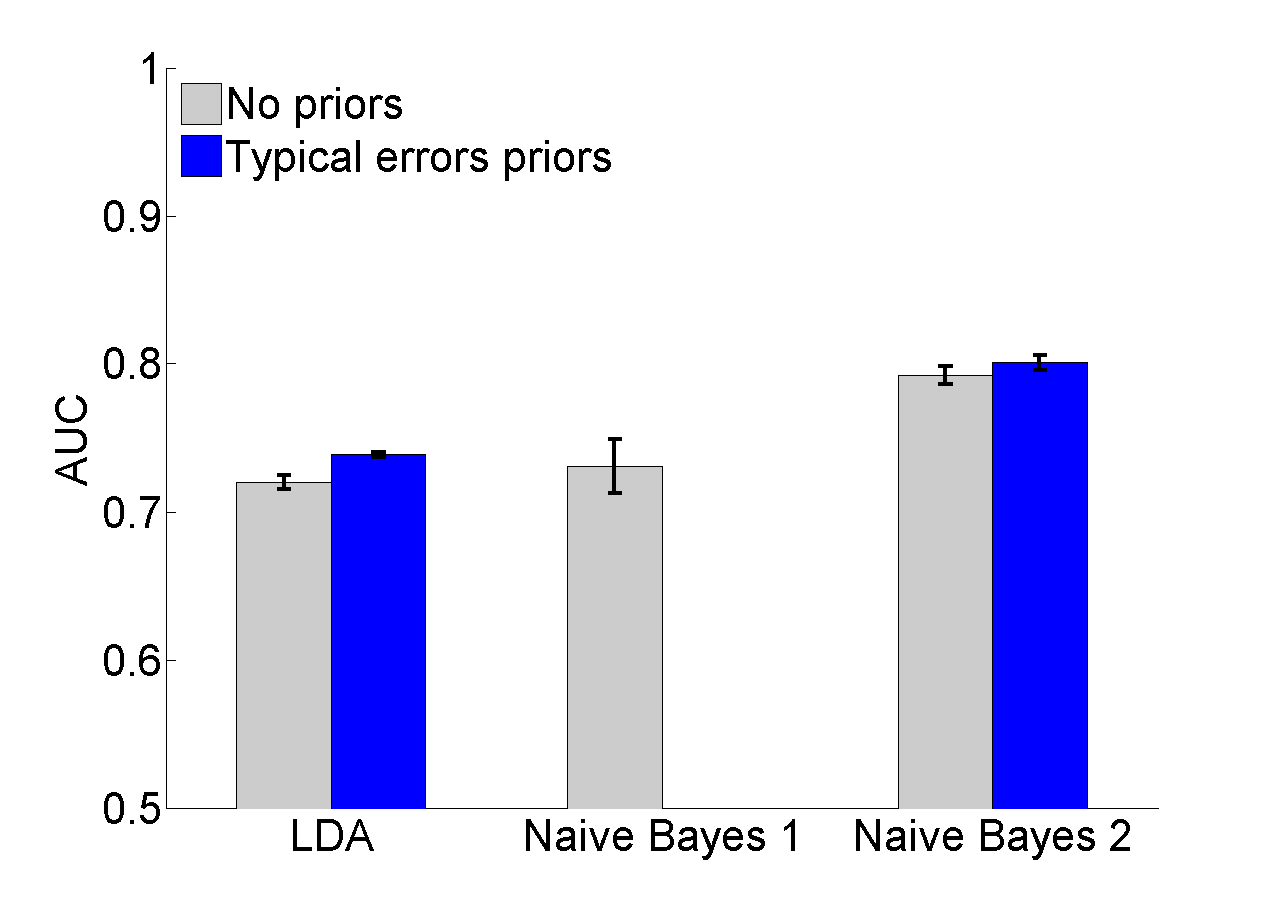
\includegraphics[width=\linewidth]{Figures/Ch1/AUC}
\caption{Accuracy results for the three graphical models – LDA, NB1 and NB2, with (dark bars) and without (light bars) typical errors priors to NB2 and LDA.}
\vspace{.3in}
\end{figure}

\begin{figure*}
\vspace{.3in}
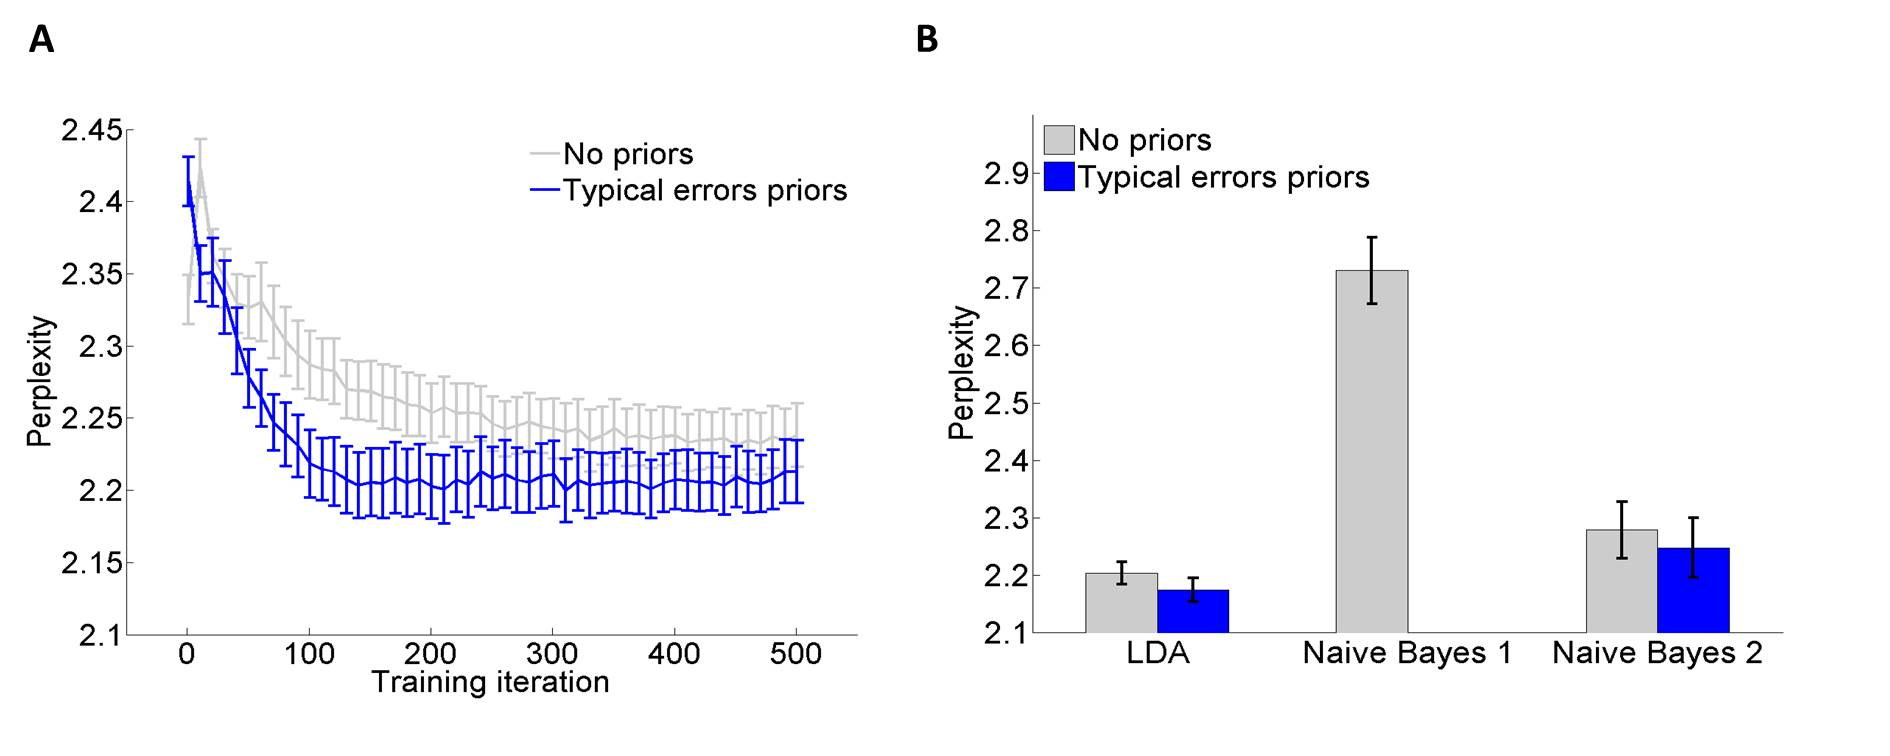
\includegraphics[width=\textwidth]{Figures/Ch1/figure5AB_HOZ}
\caption{(A) Perplexity values for the prediction set during training of the LDA model, with (dark curve) and without (light curve) typical-error priors. (B) A comparison between perplexity values calculated for the three models, with (dark bars) and without (light bars) typical-error priors to the NB2 and LDA models.}
\vspace{.3in}
\end{figure*}

 \vspace*{2\baselineskip}

Figure 1.3 shows the comparison between the accuracy of the models, table 1.1 summarizes the resulting AUC values. The highest accuracy is achieved with the NB2 model when it is provided with typical-errors priors $\beta_{wed}$. Next are the LDA when it is provided with typical-errors priors and the NB1 Models. Results reflect that the NB2 model is best at replicating diagnoses of experts, and therefore can be used as an automated data-driven tool for dyslexia diagnosis.

\begin{table}
\centering
\caption{Accuracy of the models.} 

\begin{tabular}{|c|c|c|c|} \hline
& NB1 & NB2 & LDA \\
\hline
&&&\\
Without & 0.731 & 0.792 & 0.720 \\
priors & (0.018) & (0.006) & (0.005) \\
&&&\\
\hline
&&&\\
With & --- & 0.801 & 0.739 \\
Priors &  & (0.005) & (0.002) \\
&&&\\
\hline\end{tabular}
\bigskip

AUC values for the three models, standard deviation values in parentheses
\end{table}

As expected, the LDA model reasonably correlates with expert diagnosis. Yet, it predicts the same diagnosis as experts in fewer cases than NB2. In the following section we examine whether this is ought to the LDA model being an inaccurate model of dyslexia, or rather the opposite - it may contribute to expert knowledge in capturing dyslexic phenomena.

\subsection{The predictive power of the models}
Which model of the proposed models (NB1, NB2, LDA) best captures the hidden error patterns in the data, thereby best characterizing dyslexic errors? We answer this by comparing the predictive power of the three models. We evaluate the predictive power of the models using the prediction-set (figure 1.2).
The perplexity score is commonly used in assessing the predictive power of a language model (e.g., \citealp{bnj03}). Here, it reflects the degree of "surprise" of the models to the errors made by the dyslexic person. Formally it is: 

\begin{equation}
Perplexity = \exp{\Bigg\{-\frac{\sum_{s=1}^{N_{test}} log(p(\bar{w_s}, \bar{e_s}))}{\sum_{s=1}^{N_{test}}|\bar{w_s}|}\Bigg\}}
\end{equation}

and it is evaluated on the prediction-set, where $ \bar{w_s} $ are the observed target-words and $ \bar{e_s} $ are the error types in the prediction-set of person p. $|\bar{w_s}|$ represents the number of words in the prediction-set ($|\bar{w_s}| = 98$), and $ N_{test} $ is the total number of test subjects ($ N_{test} = 219 $).

We also compare the predictive power of NB2 to LDA when provided with priors about the typical errors for each dyslexia subtype. Figure 1.4 shows that the perplexity of these models is lower when provided with priors (figure 1.4: dark curve in panel A and dark bars in panel B). Incorporating expert knowledge into the model therefore increases its predictive power.

The prior value of the diagnosis distribution was set to be uniform with arbitrary value $ \alpha_{dp} = 0.05 $. The lower prior for the word-error-dyslexia distribution was set to $ \beta_{low} = 0.05 $, whereas for the higher prior $ \beta_{high} $, different values were explored. $ \beta_{high} $ is then chosen to be the value that achieves lowest perplexity $ \beta_{high} = 0.7 $ (figure 1.3). The perplexity values for all three models are summarized in figure 1.3b.

These results show that the best prediction of reading errors is achieved by the LDA model when it is provided with typical-errors priors (figure 1.3B). This result is consistent for different typical-error priors when compared to the NB2 model (figure 4). These results indicate that the LDA model best captures the hidden structure of reading errors, among all three models.

\begin{figure}[h]
\vspace{.3in}
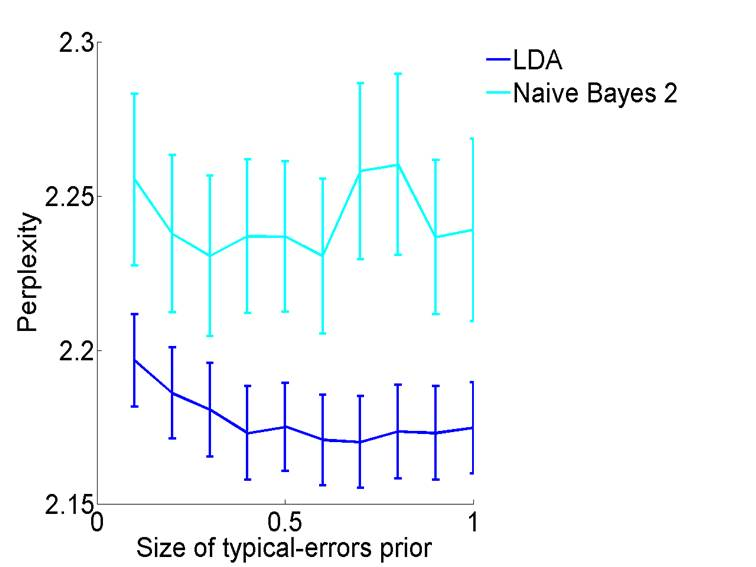
\includegraphics[width=\linewidth]{Figures/Ch1/figure5C.jpg}
\vspace{.3in}
\caption{Perplexity values calculated for the NB2 and LDA models for varying size of typical-error prior value $\beta_{high}$.}
\end{figure}

\subsection{The Dyslexia-Attention model of reading}
In addition to dyslexia, other factors may contribute to reading errors. For instance, people make reading mistakes due to momentarily lowered attention, which may be caused by an attention deficit or simply because they become tired as the diagnostic procedure progresses. These causes may interact with dyslexia. We hypothesized that we could "clean out" incorrect assignments of reading errors to dyslexia, rath\-er than to an unattended state, by disentangling errors caus\-ed by dyslexia from errors caused by low attention. We further hypothesized that by disentangling the two, we could classify between participants which are diagnosed with attention deficit disorder in addition to dyslexia. We therefore designed a model that takes into account the two possible causes of reading errors, specific dyslexia types and a generic low attention state, incorporating the manner in which these change during the diagnostic procedure. Specifically, we added to the LDA-based graphical model a binary random hidden variable marking the attentional state of the subject, attended or unattended, while reading each word. We set these attentional states as a hidden Markov chain, incorporating the dynamics of reading errors in time. We trained the model in a similar way to the LDA-based model, but this time also inferring the hidden attention states and learning the transition probabilities between these states.

When evaluating this model, as in the above experiments, we did not find the Dyslexia-Attention model to improve over the dyslexia-state LDA model. We hypothesize that two reasons may explain the lack of improvement. First, adding the attention hidden variables requires a significantly larger number of parameters, which might be hard to well optimize with the current dataset. It is possible that training the model with an even larger corpus of data would improve the predictions. A second possible reason is that the attentional processes follow a different time scale than the one captured by the current experiments. The time spent in a state in an hidden Markov model follows an exponential distribution, and this may not be an adequate model for switching between attention states. We encourage and intend to further examine this line of research with more accumulating data. 

%\vfill

\section{Discussion}
This study is a first demonstration of using probabilistic graphical models as a method for analyzing reading errors made by dyslexic people. The work has two main novel contributions: (a) it provides an automatic diagnosis tool of dyslexia, based on data of types of reading errors; (b) it provides probabilistic tools which enable exploring dyslexic phenomena based on reading errors data. By using these tools, the hidden structure of reading errors data, such as the probability of an error-type given a dyslexia and a target-word, may be extracted.

We tested three graphical models, a Latent Dirichlet Allocation (LDA) model and two Na\"{\i}ve-Bayes models, all differing by their complexity. The models were trained on a uniquely large data set of reading tests taken by dyslexic people.

Two experiments were conducted with the data to determine: (a) which model best captures the fine structure of the patterns of reading errors, and (b) which model best agrees with expert diagnoses. 

To answer the above questions, multiple models where train\-ed on a large corpus including 313 subjects and 196 target words in each test. Note that the majority of responses on the reading tests are correct responses of the subject, therefore most of the information about the structure of the errors resides in a small proportion of the data ($<20\%$). We expect accuracy of algorithms to improve as more data is accumulated.

The results show that the LDA model achieves best performance in terms of predicting reading errors, and it is therefore best in capturing the fine structure of the data. This result has both theoretical and practical implications. It may contribute to the understanding of dyslexic phenomena, and it may be used to improve designs of screening tests.

Another result of this study may serve as an application for diagnosis of dyslexia. NB2 was best in replicating diagnoses of experts ($AUC = 0.801$). This is yet another demonstration of Na\"{\i}ve-Bayes models being efficient classifiers. Note that in this study all models were trained on the screening-tests only, whereas diagnoses of clinicians are usually based on the results of the post-tests as well. The data-driven models, and particularly NB2, performed well in detecting the dyslexia subtype without leveraging the post-test information and thus are very effective.

Finally, the predictive power of the Na\"{\i}ve-Bayes and LDA models is improved when the models are provided with priors which are set according to knowledge of experts from the subtype approach. If the subtype approach were wrong, adding these priors would damage the predictive power of the model rather than improving it. The accuracy of these models is also improved when providing the models with such priors. Our work therefore provides support to the subtype approach to dyslexia, and exemplifies the ability of probabilistic graphical models to shed light on theoretical issues from different research fields, such as reading disorders in the case here.

Our vision is to deploy the algorithm of the NB2 model as a mobile application, providing an accessible, cheap and fast screening test, which allows people to obtain initial screening results, helping them decide whether further diagnosis is needed. This can be achieved by a mobile application which presents a series of words, asks the user to read them aloud, recognizes the spoken words, and uses the diagnosis algorithms described here to provide an initial diagnosis. The main challenge in achieving this is having the speech recognition component recognize utterances that are nonwords. Responses of dyslexic people may differ from existing words, whereas automatic speech recognizers (ASRs) are often trained to provide the most likely word elicited. For example, a subject may read an existing word such as \textit{cloud}, as another existing word \textit{could}, but also as a nonword such as \textit{clud}. This kind of distinction is crucial for the diagnosis. This challenge can be addressed by training and assessing ASR tools on data sets of labeled nonwords.

To conclude, this study is a demonstration of the use of probabilistic graphical models as a method of analyzing reading errors data. The progress presented in this paper can also be deployed as a novel, efficient diagnostic tool for dyslexia, based on reading errors only. The Naive-Bayes model tested in this research was compared to labels given by experts in diagnosis of dyslexia, and was found to be an accurate and reliable candidate for an automated tool for initial screening of dyslexia, by its subtypes. 

\titleformat{\chapter}[display]
{\normalfont%
    \huge% %change this size to your needs for the first line
    \bfseries}{\chaptertitlename\ \thechapter}{20pt}{%
    \Huge %change this size to your needs for the second line
    }

\titleformat{\chapter}[display]
{\normalfont%
    \tiny% %change this size to your needs for the first line
    \bfseries}{}{20pt}{%
    \LARGE %change this size to your needs for the second line
    }
%% Chapter 2
\lhead{\emph{Chapter 2: The Perceptually Discriminative Power of Subphonemic Features}}
%\input{Chapters/Ch2/abstract3.tex}
%\input{Chapters/Ch2/Intro3.tex}
\chapter{Chapter 2: Perceptual saliencies of subphonemic features}
\section{Introduction}
A common processing malfunction in speech perception is the misperception of one phoneme as another in normal or noisy conditions, usually in the context of spoken words or sentences. For example, when mishearing someone saying ‘take it’ as ‘make it’. Notably, some of phoneme substitutions are more likely than others. For example, putting aside non-phonolgical effects, it is more likely to mishear ‘take it’ as ‘fake it’ than as ‘make it’. One contributing factor for such confusions is that the pair of phonemes /t/-/f/ is more confusable with each other than the pair /t/-/m/. This raises the question: what makes one pair of phonemes more perceptually confusable, or similar \citep{Tversky1977, Shepard1987}, than another pair? Section 2.1.1 provides a brief history of the main developments of phonological theories, described according to two lines of research - auditory and gestural theories. Section 2.1.2 discusses phoneme-similarity theories and the empirical approach to phoneme similarity. Finally, section 2.1.3 presents a new methodological approach to the problem.  

\subsection{Feature theories}
Speech sounds often exhibit the same behavior, grouping together into sound patterns in spoken languages. For example, in German, the singular and plural forms consistently differ by specific pairs of sounds, such as /b/-/p/ in the German word for 'robbery': Raube vs. Raub (final b pronounced as /p/); or for 'bath': /d/-/t/ in  Bäder  vs. Bad (final d pronounced as /t/), and /g/-/k/, /z/-/s/ and /v/-/f/ in other cases. All these different pairs of phonemes have a single property in common: in the plural form, the sounds (/bgdvz/) always include voicing - a vibration of the vocal chords during pronunciation, which has identifiable acoustic markers - whereas in the singular form, the corresponding sounds are unvoiced. Such groups of sounds are termed \textit{natural classes} and they are denoted by subphonemic features, such as [-voice] and [+consonantal]. Natural classes are typically affected, and affect other sounds, in the same way in the same environment, as in the above example. It was therefore suggested that phonological alterations, such as the devoicing process, act on subphonemic features rather than on the phonemic segments themselves. Interestingly, different languages may present similar to identical processes. For example, in Turkish, similarly to German, we find final devoicing in, e.g., 'kitabim' ('my book') vs. 'kitap' ('book'), or 'a\u{g}aim' ('my tree') vs. 'a\u{g}a\c{c}' ('tree'). Such similarities have led to the hypothesis that phonological features are universal and innate (\citealp{ChomskyHalle1968}, but see \citealp{mielke2008emergence}).

\paragraph{Auditory theories}
Around the mid of the 20$^{th}$ century, \citet{jakobson1951preliminaries} suggested that phonological patterns in all languages can be described with only a limited number of contrasting features, such as, voiced-unvoiced, strident-mellow, or nasal-oral. According to this theory, all features can be assigned a unique acoustic correlate, which in turn, correspond to specific articulatory parameters. The articulatory stage, however, is viewed as a mere mechanism to generate acoustic contrasts - "we speak to be heard in order to be understood" (ibid.), and features do not necessarily have a unique articulatory correlate. This line of research, emphasizing the acoustic aspect of distinctive features, was later developed by \textit{the quantal theory of speech perception} \citep{stevens1972quantal,stevens1989quantal}. This theory added to the field by characterizing the interactions between articulatory parameters of speech and their acoustic outcomes. It suggested that the mapping between articulation to acoustics is highly non-linear, with stable regions (small changes in the articulator have small acoustic effects) and unstable regions (small changes in the articulator generate large acoustic effects). The discontinuities around the unstable regions are used to define the boundaries between features. In this way, the theory accounts for a fundamental question in the field - why languages distinctly favor certain articulatory and acoustic dimensions in constructing their phoneme inventories, while avoiding others. The quantal theory explains this by defining optimality of features - a feature is optimal if it maximizes the difference between phonemes in the auditory space while preserving minimal articulatory effort. This phonological economy explains why features are universal, as they are dependent on biological properties of the human speech-production system, which are essentially the same for all humans.

\paragraph{Gestural theories}
From around the middle of the 20$^{th}$ century, a competing view to auditory theories was developed, called {\it The Motor Theory of Speech Perception} \citep{cooper1952some, liberman1967perception}. Its primary motivation stemmed from the observation that acoustic waveforms of synthetic speech have to be modified in order to produce a constant perception of the same phoneme in different phonological contexts. It was therefore concluded that the objects of speech perception cannot be found in acoustics, in contrast to the view of auditory theories, but should rather be anchored in articulatory gestures. Accordingly, during speech perception, the hearer extracts the intended phonetic gestures of the speaker \citep{liberman1985motor}, rather than acoustic cues. Phonemes are thus viewed as groups of gestural features. In a later theory in the same thread of research, giving emphasis to articulation as well, \citet{ChomskyHalle1968} suggested that phonological patterns across languages can be accounted for with an innate set of articulatory features. Importantly, they argue that what is perceived depends not only on the physical constitution of the signal but also on the linguistic knowledge of the hearer, introducing top-down and expectation processes into the field of speech perception. A further development of this line of research, called feature geometry \citep{clements1985, sagey1986representation}, suggested that speech sounds have an internal featural structure, rather than being comprised of a "bundle" of features. In its simple form, the theory describes the internal structure of segments in terms of a tree, whose nodes are features, higher levels are feature classes and, finally, the root node represents the entire object. Describing sounds with trees enabled the theory to account for phonological patterns in a more parsimonious way compared to previous theories. More recently, \citet{browman1990tiers, browman1992articulatory} suggested a model of gestural coordination known as \textit{Articulatory phonology}. Their underlying hypothesis is that spoken language is best described by patterns of coordinated articulatory gestures. The theory proposes to model phonetic and phonological patterns in terms of "articulatory scores", which are formal representations consisting of abstract gestures and their patterns of coordination.


\subsection{Theories for phoneme similarity}
\paragraph{Feature-based approach}
Phoneme similarity is traditionally explained by decomposing phonemes into subphonemic features, assuming the more features two phonemes share the more similar they are \citep{Tversky1977, Shepard1987, Cohen2009, Cohen2010}. Given a feature theory, a metric (distance) or a phoneme-similarity functions can be defined over pairs of phonemes. For example, given the three contrastive articulatory dimensions - voicing, place- and manner-of-articulation - a common similarity function in psycholinguistics is to count the number of dimensions on which two phonemes agree (e.g., \citealp{mcmillan2010cascading, Bailey2005, mousikou2015masked}). For instance, the phoneme /b/ is labial-plosive-voiced, and the phoneme /g/ is velar-plosive-voiced. The similarity score for these two phonemes is thus two. Other, more sophisticated, similarity measures have been proposed in the literature. These include a similarity measure based on the number of shared and non-shared features \citep{Pierrehumbert1993}, or on the number of shared and non-shared natural classes \citep{Frisch1997}. According to this last measure, similarity between two phonemes is the proportion of natural classes that are shared by the two phonemes, compared to the total shared and not-shared natural classes. Features are thus assigned weights according to their redundancy. Therefore, different features contribute differently in explaining perceptual distances, since redundant features affect similarity less than non-redundant features.

\paragraph{Experimental approach}
Another approach to phoneme similarity addresses the problem by quantifying perceptual phoneme similarities directly in an experiment. Typically, such experiments present noise-corrupted phonemes to subjects, collecting their perceptual judgments of phoneme identity \citep{NicelyMiller1955}. Confusion matrices are then derived from the data, mapping the likelihood that any given phoneme is confused with another phoneme. This approach has been widely used, however, there are several associated concerns that should be kept in mind. First, phoneme confusions may depend on the noise characteristics added to the signal. For example, results from phoneme-confusion experiments using white noise (e.g., \citealp{NicelyMiller1955, Luce1987}) may differ from those that use pink noise (e.g., \citealp{redford1999relative}), or speech-shaped ('babble') noise \citep{cutler2004patterns}. Another source of variability is due to context effects. These may have large effects on perceptual confusability, in particular, consonant confusions may be different when the consonant is in initial or final position of the word \citep{Luce1987, hura1992role, redford1999relative}. Finally, phoneme perception shows asymmetric effect \citep{kuhl1991human}, which was addressed by several feature theories. For example, the featurally underspecified lexicon (FUL) theory \citep{lahiri2002underspecified, lahiri2010distinctive} accounts for asymmetry effects by stating that some features are universally underspecified. For instance, the feature [coronal] is underspecified in the lexicon, which prevents mismatches between labial or dorsal sounds that are detected in the signal, and allows them to access the lexicon. In contrast, labial and dorsal features are specified, and so a coronal sound detected in the signal will mismatch both of these features, and cannot access the lexicon. In speech production, \citet{Frisch1997} claims that similarity neighborhoods in the mental lexicon affect asymmetries in sound substitutions.

\subsection{A metric-learning approach}
We now describe a general framework that we suggest as a new methodological approach to the problem of phoneme similarity. The approach allows the integration of various effects, such as context or asymmetry, into its framework, and is compatible with various feature theories - e.g., auditory or gestural, and with any choice of noise characteristics in phoneme-confusion experiments - white, pink or speech-shaped.

Traditionally, feature-based theories, such as the ones described above, craft a similarity or a metric function based on theoretical insights and intuition. However, current theoretical metrics do not fully account for empirical perceptual distances (e.g. \citealp{Bailey2005}). One reason for this may be that theoretical metrics misevaluate or underestimate the difference in contribution of each subphonemic feature to perceptual distances. 

In this study, we explore an approach that learns a metric function directly from the data, assuming only its general form. For this, we parametrize a general metric function and derive its values using learning algorithms. A geometric interpretation of this approach is illustrated in figure 2.1. Given a feature theory, phonemes can be represented as points in feature space, in which dimensions correspond to subphonemic features (figure 2.1 left). The set of all Euclidean distances between phonemes in this space likely differ from the set of the empirical ones (figure 2.1 right), which were derived from, e.g., a phoneme-confusion data. Given this discrepancy between the two structures, we look for an optimal mapping between the two spaces, such that the distances from the feature space will match as closely as possible the set of distances from the experiment (figure 2.1 middle arrow). This optimal mapping defines a metric function over pairs of phonemes. Importantly, once the optimal mapping is derived from the data, one can learn about the perceptually discriminative power of the various features. As an example, if the mapping is linear and represented by a (positive) diagonal matrix, the mapping amounts to stretchings or contractions of the feature dimensions. Dimensions that are relatively highly stretched would thus correspond to features that are more perceptually discriminative.

\begin{figure}
\vspace{.3in}
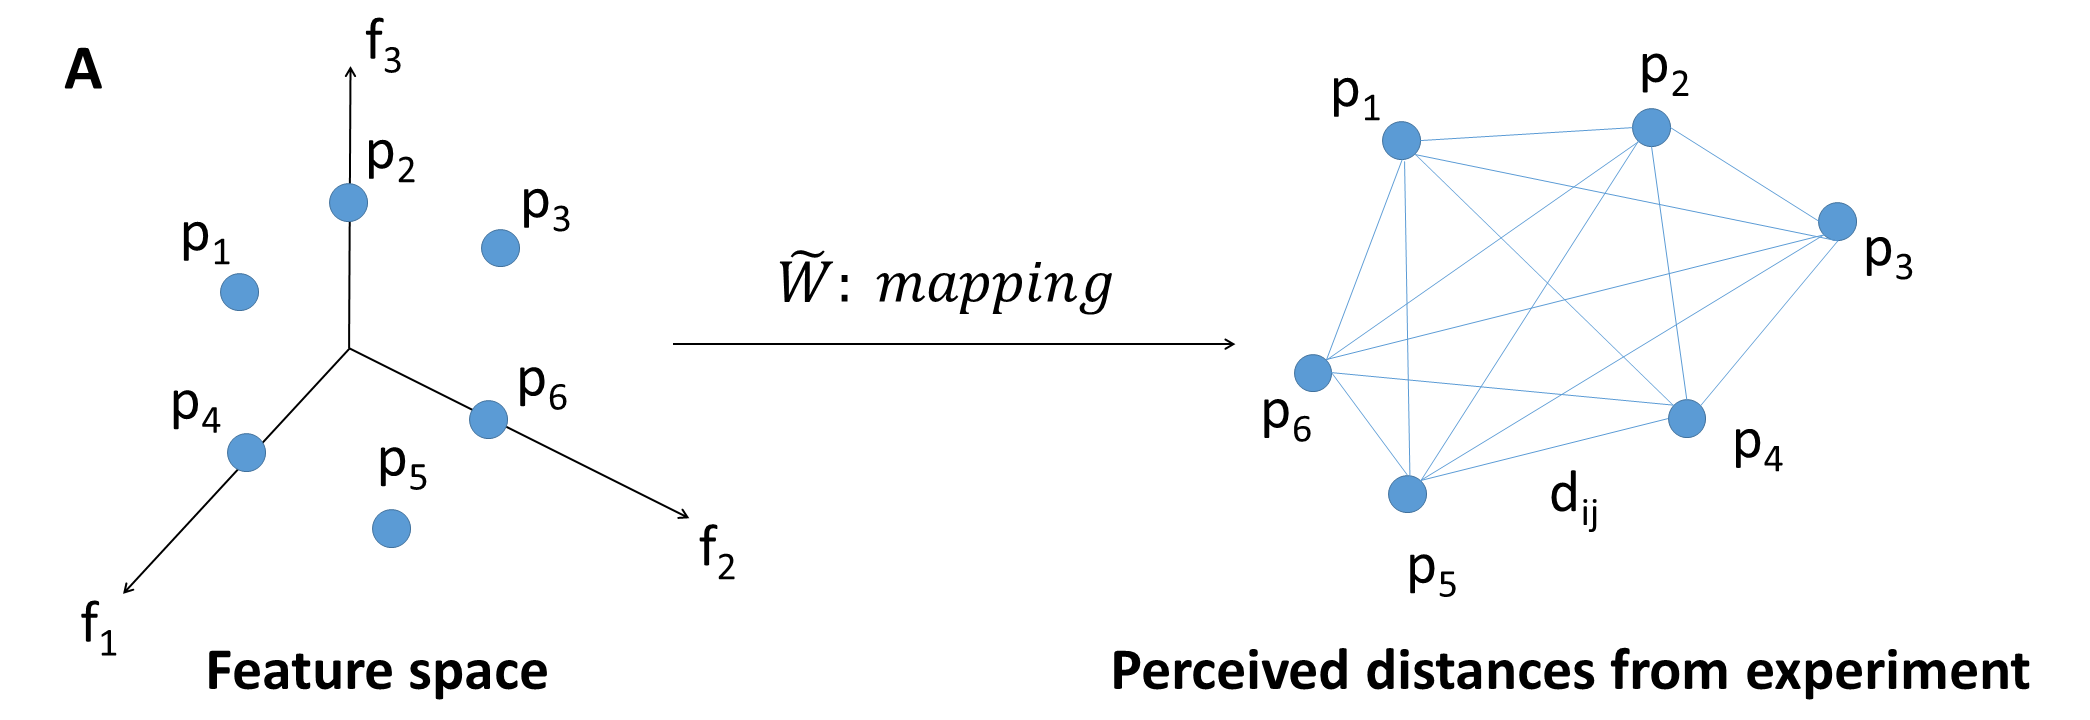
\includegraphics[width=\linewidth]{Figures/Ch2/Figure1_2017Sep10.png}
\caption{An illustration of metric learning for phonemes: phonemes $p_i's$ are represented in a feature space (left), where each dimension corresponds to a feature. Perceptual distances as collected in an experiment $d_{ij}$ (right) are used to learn an optimal mapping (middle arrow), defined over the feature space. The mapping is optimal in the sense that it maps the phonemes from the feature space such that the distances between the mapped phonemes are as close as possible to the empirical ones.}
\end{figure}

We test our approach on two English phoneme-confusion datasets \citep{NicelyMiller1955, Luce1987} and a new dataset that we have collected for Hebrew. In all cases, we focus on consonant confusions at initial position and white noise in all experiments. In addition, we present and compare several alternatives to learn the metric function. For computational convenience, we assume a linear mapping and a symmetric metric function. However, the approach can be pursued with a removal of such assumptions, as we later discuss.
\section{Methods}
We describe learning a metric given a feature set and a phoneme-similarity dataset. Section 2.2.1 describes phoneme representations in feature space. Section 2.2.2 describes different methods for learning optimal mappings. Finally, Section 2.2.3 describes phoneme-confusion datasets that are used in this study, and the way perceptual distances were estimated.

\subsection{Representing phonemes in feature space}
We study phoneme representations in the feature space based on: (a) Articulatory features, and (b) Phonological features. See table 2.1 for the full list of phonemes.

\paragraph{Articulatory features} The first representation scheme uses 14 binary features, based on articulatory features: six place features - labial, dental, alveolar, palatal, velar and glottal, ordered according to the place along the vocal tract (Figure 1B); Seven manner features - plosive, fricative, affricate, lateral, rhotic, nasal, glide, ordered by sonority; And a single voicing feature. As an example, the labial-plosive-unvoiced /p/ is represented  as (1, 0, 0, 0, 0, 0, 0, 1, 0, 0, 0, 0, 0, 0), where the first six components are for place of articulation, the next seven components are for manner and the last vector component is for voicing. Another example, the alveolar-nasal-voiced /n/ is represented as (0, 0, 0, 0, 1, 0, 0, 0, 0, 0, 0, 1, 0, 1).

\paragraph{Phonological features} Phonemes are represented along 12 binary phonological features: consonantal, continuant, strident, voicing, nasality, dorsal, anterior, labial, coronal, distributed and lateral. Continuing with the above examples, /p/ is represented here as (1, 0, 0, 0, 0, 0, 0, 0, 1, 0, 0, 0); and /n/ is represented as (1, 0, 0, 0, 1, 1, 0, 1, 0, 1, 0, 0). \mbox{} \\

Both representation schemes include the minimal set of features that is required to distinguish among all phonemes in the English and Hebrew datasets. Adding more features introduces redundancy among the features. For example, to distinguish between the sets of phonemes in the datasets, the sonority feature is not required in addition to the above list of features. Adding it would introduce redundancy with, e.g., the voicing feature, which might reduce the predictive power of the metric function and its interpretability.


\begin{landscape}% Landscape page

\begin{table}[H]
\centering % Center table
\tiny
\begin{tabular}{|c|c|c|c|c|c|c|c|c|c|c|c|c||c|c|c|c|c|c|c|c|c|c|c|c|c|c|}
\hline

&\multicolumn{12}{|c|}{Phonological features}&\multicolumn{14}{|c|}{Articulatory features}\\
\hline
&	cn	&	ct	&	DR	&	st	&	vc	&	ns	&	dr	&	an	&	lb	&	cr	&	ds	&	lt	&	lb	&	dn	&	al	&	pa	&	vl	&	gl	&	pl	&	af	&	fr	&	ns	&	lt	&	rt	&	gd	&	vc	\\
\hline

${p}^{\star\dagger\ddagger}$	&	+	&	-	&	-	&	-	&	-	&	-	&	-	&	-	&	+	&	-	&	-	&	-	&	+	&	-	&	-	&	-	&	-	&	-	&	+	&	-	&	-	&	-	&	-	&	-	&	-	&	-	\\
$b^{\star\dagger\ddagger}$	&	+	&	-	&	-	&	-	&	+	&	-	&	-	&	-	&	+	&	-	&	-	&	-	&	+	&	-	&	-	&	-	&	-	&	-	&	+	&	-	&	-	&	-	&	-	&	-	&	-	&	+	\\
$t^{\star\dagger\ddagger}$	&	+	&	-	&	-	&	-	&	-	&	-	&	-	&	+	&	-	&	+	&	-	&	-	&	-	&	-	&	+	&	-	&	-	&	-	&	+	&	-	&	-	&	-	&	-	&	-	&	-	&	-	\\
$d^{\star\dagger\ddagger}$	&	+	&	-	&	-	&	-	&	+	&	-	&	-	&	+	&	-	&	+	&	-	&	-	&	-	&	-	&	+	&	-	&	-	&	-	&	+	&	-	&	-	&	-	&	-	&	-	&	-	&	+	\\
$k^{\star\dagger\ddagger}$	&	+	&	-	&	-	&	-	&	-	&	-	&	+	&	-	&	-	&	-	&	-	&	-	&	-	&	-	&	-	&	-	&	-	&	-	&	+	&	-	&	-	&	-	&	-	&	-	&	-	&	-	\\
$g^{\star\dagger\ddagger}$	&	+	&	-	&	-	&	-	&	+	&	-	&	+	&	-	&	-	&	-	&	-	&	-	&	-	&	-	&	-	&	-	&	-	&	-	&	+	&	-	&	-	&	-	&	-	&	-	&	-	&	+	\\
\textipa{tS}$^{\star}$	&	+	&	-	&	+	&	+	&	-	&	-	&	-	&	-	&	-	&	+	&	+	&	-	&	-	&	-	&	-	&	+	&	-	&	-	&	-	&	+	&	-	&	-	&	-	&	-	&	-	&	-	\\
\textipa{dZ}$^{\star}$	&	+	&	-	&	+	&	+	&	+	&	-	&	-	&	-	&	-	&	+	&	+	&	-	&	-	&	-	&	-	&	+	&	-	&	-	&	-	&	+	&	-	&	-	&	-	&	-	&	-	&	+	\\
$f^{\star\dagger\ddagger}$	&	+	&	+	&	-	&	-	&	-	&	-	&	-	&	-	&	+	&	-	&	-	&	-	&	+	&	-	&	-	&	-	&	-	&	-	&	-	&	-	&	+	&	-	&	-	&	-	&	-	&	-	\\
$v^{\star\dagger\ddagger}$	&	+	&	+	&	-	&	-	&	+	&	-	&	-	&	-	&	+	&	-	&	-	&	-	&	+	&	-	&	-	&	-	&	-	&	-	&	-	&	-	&	+	&	-	&	-	&	-	&	-	&	+	\\
\textipa{T}$^{\star\dagger}$	&	+	&	+	&	-	&	-	&	-	&	-	&	-	&	+	&	-	&	+	&	-	&	-	&	-	&	+	&	-	&	-	&	-	&	-	&	-	&	-	&	+	&	-	&	-	&	-	&	-	&	-	\\
\textipa{D}$^{\star\dagger}$	&	+	&	+	&	-	&	-	&	+	&	-	&	-	&	+	&	-	&	+	&	-	&	-	&	-	&	+	&	-	&	-	&	-	&	-	&	-	&	-	&	+	&	-	&	-	&	-	&	-	&	+	\\
$s^{\star\dagger\ddagger}$	&	+	&	+	&	-	&	+	&	-	&	-	&	-	&	+	&	-	&	+	&	-	&	-	&	-	&	-	&	+	&	-	&	-	&	-	&	-	&	-	&	+	&	-	&	-	&	-	&	-	&	-	\\
$z^{\star\dagger\ddagger}$	&	+	&	+	&	-	&	+	&	+	&	-	&	-	&	+	&	-	&	+	&	-	&	-	&	-	&	-	&	+	&	-	&	-	&	-	&	-	&	-	&	+	&	-	&	-	&	-	&	-	&	+	\\
\textipa{S}$^{\star\dagger\ddagger}$	&	+	&	+	&	-	&	+	&	-	&	-	&	-	&	-	&	-	&	+	&	+	&	-	&	-	&	-	&	-	&	+	&	-	&	-	&	-	&	-	&	+	&	-	&	-	&	-	&	-	&	-	\\
\textipa{Z}$^{\dagger}$	&	+	&	+	&	-	&	+	&	+	&	-	&	-	&	-	&	-	&	+	&	+	&	-	&	-	&	-	&	-	&	+	&	-	&	-	&	-	&	-	&	+	&	-	&	-	&	-	&	-	&	+	\\
$h^{\star\dagger\ddagger}$	&	+	&	+	&	-	&	-	&	-	&	-	&	-	&	-	&	-	&	-	&	-	&	-	&	-	&	-	&	-	&	-	&	-	&	+	&	-	&	-	&	+	&	-	&	-	&	-	&	-	&	-	\\
$m^{\star\dagger\ddagger}$	&	+	&	-	&	-	&	-	&	+	&	+	&	-	&	-	&	+	&	-	&	-	&	-	&	+	&	-	&	-	&	-	&	-	&	-	&	-	&	-	&	-	&	+	&	-	&	-	&	-	&	+	\\
$n^{\star\dagger\ddagger}$	&	+	&	-	&	-	&	-	&	+	&	+	&	-	&	+	&	-	&	+	&	-	&	-	&	-	&	-	&	+	&	-	&	-	&	-	&	-	&	-	&	-	&	+	&	-	&	-	&	-	&	+	\\
\textipa{N}$^{\star}$	&	+	&	-	&	-	&	-	&	+	&	+	&	+	&	-	&	-	&	-	&	-	&	-	&	-	&	-	&	-	&	-	&	+	&	-	&	-	&	-	&	-	&	+	&	-	&	-	&	-	&	+	\\
$l^{\star\ddagger}$	&	+	&	+	&	-	&	-	&	+	&	-	&	-	&	+	&	-	&	+	&	-	&	+	&	-	&	-	&	+	&	-	&	-	&	-	&	-	&	-	&	-	&	-	&	+	&	-	&	-	&	+	\\
\textipa{R}$^{\star}$	&	+	&	+	&	-	&	-	&	+	&	-	&	-	&	-	&	-	&	+	&	-	&	-	&	-	&	-	&	+	&	-	&	-	&	-	&	-	&	-	&	-	&	-	&	-	&	+	&	-	&	+	\\
$w^{\star}$	&	-	&	+	&	-	&	-	&	+	&	-	&	+	&	-	&	+	&	-	&	-	&	-	&	+	&	-	&	-	&	-	&	-	&	-	&	-	&	-	&	-	&	-	&	-	&	-	&	+	&	+	\\
$j^{\star\ddagger}$	&	-	&	+	&	-	&	-	&	+	&	-	&	-	&	-	&	-	&	+	&	+	&	-	&	-	&	-	&	-	&	+	&	-	&	-	&	-	&	-	&	-	&	-	&	-	&	-	&	+	&	+	\\
\textipa{X}$^{\ddagger}$	&	+	&	+	&	-	&	-	&	-	&	-	&	+	&	-	&	-	&	-	&	-	&	-	&	-	&	-	&	-	&	-	&	+	&	-	&	-	&	-	&	+	&	-	&	-	&	-	&	-	&	-	\\
\textipa{ts}$^{\ddagger}$	&	+	&	-	&	+	&	+	&	-	&	-	&	-	&	+	&	-	&	+	&	-	&	-	&	-	&	-	&	+	&	-	&	-	&	-	&	-	&	+	&	-	&	-	&	-	&	-	&	-	&	-	\\
\textipa{K}$^{\ddagger}$	&	+	&	+	&	-	&	-	&	+	&	-	&	+	&	-	&	-	&	-	&	-	&	-	&	-	&	-	&	-	&	-	&	+	&	-	&	-	&	-	&	-	&	-	&	-	&	+	&	-	&	+	\\

\hline

\end{tabular}

\caption{Phonological and articulatory features of all phonemes in the datasets. cn=consonantal; ct=continuant; DR=delayed release; st=strident; vc=voicing; ns=nasal; dr=dorsal; an=anterior; lb=labial; cr=coronal; ds=distributed; lt=lateral; dn=dental; al=alveolar; pa=postalveolar; vl=velar; gl=glottal; pl=plosive; af=affricate; fr=fricative; lt=lateral; rt=rhotic; gd=glide. $^{\star}$Luce, $^{\dagger}$N\&M, $^{\ddagger}$Hebrew dataset}

\end{table}
\end{landscape}

\subsection{Metric learning}
We explore two approaches to learn a metric function \citep{Kulis2012}: (1) viewing the problem as a least-squares problem and (2) viewing the problem as a large-margin ranking problem \citep{Chechik2010}. We begin by providing a formal definition of the problem, describing the terms, variables and parameters of the proposed model.

Let $A$ be a set, a metric function $d: A \times A \to \mathbb{R}$ is a non-negative symmetric function over pairs of elements of $A$, which assigns a value (a distance) to every pair in the set, and satisfies the triangle inequality and that for every element $x$ in $A$: $d(x, x) = 0$.

In our case, the elements of the set are phonemes $\{\bar{p}^1, ..., \bar{p}^{n_p}\}$, where $n_p$ is the number of phonemes. We describe each phoneme as a vector of size $n_f$, $\bar{p}^i \in \mathbb{R} ^{n_f}$, and define the following metric $d_{ij}(\bar{p}^i, \bar{p}^j)$ over pairs of phonemes:

\begin{equation}
    d_{ij}(\bar{p}^i, \bar{p}^j) = (\bar{p}^i - \bar{p}^j)^T W (\bar{p}^i - \bar{p}^j),
\end{equation}

where $W \in \mathbb{R} ^{n_f \times n_f}$ is a positive semi-definite (PSD) real-valued matrix. This function is a proper metric since it satisfies all conditions: non-negativity (PSD), symmetry, the triangle inequality, and that the distance between a phoneme to itself is always zero. 

Geometrically, this metric can be described as: (1) performing a linear mapping on a given pair of vectors from the feature space; and (2) calculating the square Euclidean distance between the results. To see this, note that a PSD matrix $W$ can be decomposed such that $W = \widetilde{W}^T\widetilde{W}$. Given a pair of phoneme vectors, $\bar{p}^i$ and $\bar{p}^i$, the mapped vectors are $\widetilde{W}\bar{p}^i$ and $\widetilde{W}\bar{p}^j$, and the square Euclidean distance between a pair of mapped phonemes is therefore: $||\widetilde{W}\bar{p}^i - \widetilde{W}\bar{p}^j||^2 = (\bar{p}^i - \bar{p}^j)^T\widetilde{W}^T\widetilde{W}(\bar{p}^i - \bar{p}^j)$, which is the right-hand side of Eq(2.1).

The free parameters of the model are the elements of $W$. Given a set of perceived distances ${D_{ij}}$ between phonemes, as measured in an experiment, an optimal set of model parameters $W^\ast$ would bring the model distances $d_{ij}$ as close as possible to the empirical distances $D_{ij}$. Formally, we define the optimization problem:

\begin{equation}
    W^\ast = \min_{W \in S^n_+}{{\sum_{{i} < {j}}{(d_{ij} - D_{ij})^2}}},
\end{equation}

where the sum is over all ${n_p \choose 2}$ pairs of phonemes, and $S^n_+$ denotes the set of $n \times n$ PSD matrices. We describe below two methods to solve the optimization problem. The first reduces the problem into a least-squares (LS) problem, the second reduces it into a large-margin ranking problem (OASIS, \citealp{Chechik2010}). We also test a variant of each of the methods, by adding a diagonal constraint on the weight matrix (section 2.2.2.3), thus having four methods in total. We refer to these four ways of learning a metric function: LS, diagonal-LS, OASIS, diagonal-OASIS.

\subsubsection{Method A: a least-squares formulation}
Formulating the problem as a least-squares problem will allow the use of standard tools to solve the problem. We now show how the problem of metric learning as defined in section 2.2.2, can be described as a least-squares problem:

We define a loss function $\mathcal{L}$ that correspond to the optimization problem in Eq(2.2).

\begin{equation}
    \mathcal{L} = \sum_{{i} < {j}}{((\bar{p}^i - \bar{p}^j)^TW(\bar{p}^i - \bar{p}^j) - D_{ij})} + \lambda||w||_1^2 \quad ,
\end{equation}

where L1-regularization is added to the loss function in its second term. Adding L1-regularization has two advantages. First, it mitigates overfitting to the empirical training data. Second, L1-regularization results in sparser solutions, i.e., a larger number of parameters have values equal to zero \citep{Tibshirani1996}. Importantly, in our case, where feature weights are derived from data collected from a perceptual-discrimination task, non-zero weights that endured this penalty are those that are necessary for explaining the measured perceptual distances. Features that have higher weight are therefore more perceptually discriminative. 

Rewriting the first term in the objective function, we get a classic LS formulation in the following matrix notation: $||\widetilde{P}\bar{w} - D||_2^2 + \lambda||w||_1^2$, where $\bar{w}$ is an $n_f^2$-dimensional vector, and $\widetilde{P}$ is an ${n_p \choose 2} \times n_f^2$ matrix. A row of $\widetilde{P}$ corresponds to the distance between the $i^{th}$ and $j^{th}$ phonemes, and a column corresponds to the weight of the $k^{th}$ and $l^{th}$ features from the quadratic form in Eq(2.1). The elements of $\widetilde{P}$ are therefore of the form: $(p_k^i-p_k^j)(p_l^i-p_l^j)$.

To solve the L1-regularized least-squares problem, we use the LASSO algorithm \citep{Tibshirani1996}. The regularizer size $\lambda$ is determined by comparing predictions of models with different values of $\lambda$'s. Values of $\lambda$ were examined for 18 values in the range $[10^{-3}, 10^5]$. The optimal size of $\lambda$ was determined according to the maximal prediction on a validation set. We refer to this method of learning a metric function as LS.

\subsubsection{Method B: a large-margin ranking problem} The goal here is to learn a metric function $d(p^i, p^j)$ as in Eq(2.1), that obeys the following condition \citep{Chechik2010}: a pair of phonemes ($p^i, p^i_+$) that are perceptually closer than another pair ($p^i, p^i_-$), are also closer according to the learned metric function. Formally, for all triplets of phonemes:

\begin{equation}
\forall{p^i, p^i_+, p^i_-}: D(p^i, p^i_+)<D(p^i, p^i_-) \rightarrow d(p^i, p^i_+)<d(p^i, p^i_-)
\end{equation}

The hinge-loss function to the constraint in Eq(2.4) together with a margin is:
\begin{equation}
    l_W(p^i, p^i_+, p^i_-) = max\{0, 1 + d(p^i, p^i_+) - d(p^i, p^i_-)\}.
\end{equation}

The optimization problem and the algorithm are then solved as in \citet{Chechik2010}. We refer to this method as OASIS.

Note that in the LS method, the exact values from the empirical data are used to learn the parameters of the model $W$, whereas in OASIS, the data values are used for ranking the empirical distances between phonemes. It is an empirical matter which of the two methods better fits our problem, we therefore explore metric learning of phonemes with both LS and OASIS.

\subsubsection{Diagonal constraint} In addition, we test a version of the above two methods when a diagonal-constraint on the parameter matrix $W$ is added. That is, the off-diagonal weights in $W$ are set to zero. The advantage of adding a diagonal constraint is that the model has fewer parameters and it is thus less prone to overfitting. On the other hand, too simple a model may not be able to capture the full structure of the data. We test each method with and without a diagonal constraint. 

\subsection{Baseline methods}
We compare the predictions of the models to three baselines: \textit{uniform weights}, \textit{PMV} \citep{ladefoged2014course} and \textit{Frisch similarity \citep{Frisch1997}}.

\paragraph{Baseline \#1: Uniform weights} $W$ is the identity matrix, with all weights set to 1 on the diagonal, and all other weights to zero.

\paragraph{Baseline \#2: Place-Manner-Voicing (PMV)} A common measure of phoneme similarity counts the number of articulatory dimensions - place, manner and voicing - that are shared by two phonemes. Formally,

\begin{equation}
S_{PMV}(p_i, p_j) = \delta_{place(p_i),place(p_j)} + \delta_{manner(p_i),manner(p_j)} + \delta_{voicing(p_i),voicing(p_j)} \quad ,
\end{equation}

where $\delta_{i,j}$ is the Kronecker delta.

\paragraph{Baseline \#3: Frisch similarity \citep{Frisch1997}} Similarity is calculated based on shared and non-shared natural classes, instead of features:
 
\begin{equation}
\resizebox{.9\hsize}{!}{$S_{FRISCH}(p_i, p_j) = \frac{\#(shared \quad natural \quad classes)}{\#(shared \quad natural \quad classes) + \#(non-shared \quad natural \quad classes)}$}.
\end{equation}

By introducing natural classes, similarity becomes dependent on the redundancy of the features. Non-redundant features have more affect on similarity than redundant ones. In particular, a totally redundant feature adds no new natural classes and therefore does not affect similarity. This introduces a weighing to the similarity function that is based on redundancy. \mbox{} \\

\subsection{Perceptual distances from confusion data}
We now describe how the perceived distances ${D_{ij}}$ are estimated from empirical data. First, phoneme similarity is calculated from confusion data following Shepard's method:

\begin{equation}
    S_{ij}=\frac{p_{ij}+p_{ji}}{p_{ii}+p_{jj}},
\end{equation}

where $p_{ij}$ is the proportion of times that $i$ tokens were called $j$. Perceived distances are then calculated following Shepard's law \citep{Shepard1987, Johnson2004}:

\begin{equation}
    D(p^i, p^j) = -ln(S(p^i, p^j)).
\end{equation}

This assumes that the relationship between perceptual distances and similarity is exponential. \citet{Ennis1988} showed that this law can account for various empirical findings about object confusion (in same-different tasks) if decisions between objects are described in a probabilistic framework. That is, percepts are treated as probabilistic and Shepard's law is applied at the stage of decision between objects.

\subsection{Model evaluation}
To compare the quality of the proposed methods, we evaluate the predictive power of the metric function of each method using a cross-validation procedure. First, for each method, we learn a metric function from a subset of the data. We then assess the prediction of the learned function on left-out data. We repeat this by leaving out a different subset of the data each time, finally averaging the resulting predictions across all left-out subsets. More specifically, we use a leave-one-phoneme-out procedure, where each time, we leave out all perceived distances involving one phoneme. We then repeat this for all phonemes. Finally, we report the average of all resulting values. 

We use the Spearman rank correlation coefficient as a prediction measure. For each left-out phoneme $p$, we calculate the Spearman correlation $\rho_{d^p, D^p}$, between the model-predicted distances to the left-out phoneme $d^p$, and the empirical ones $D^p$. The final evaluation measure of model prediction is the average of this measure across all left-out phonemes $\bar{\rho} = \frac{1}{n_p}\sum_{p=1}^{n_p}\rho_{d^p, D^p}$. According to the distribution of the values $\rho_{d^p, D^p}$ we evaluate statistical significance between different methods.
\section{The data}
Confusion errors have traditionally been used as a measure for perceptual phoneme similarity, based on the idea that the more confusable two phonemes are the more similar they are. Three phoneme-confusion datasets are explored in this study: (1) the dataset from \citet{NicelyMiller1955}, (2) The dataset from \citet{Luce1987}, and (3) results from our experiment in Hebrew.

\subsection{The Nicely and Miller dataset} The classic work by \citet{NicelyMiller1955} analyzed auditory confusion between pairs of 16 consonant phonemes of English with added white noise at different signal-to-noise ratios (SNRs). The noise-corrupted phonemes were presented to subjects in a classification-task paradigm, in a consonant-vowel (CV) form, and the effect of low- and high-pass filtering on phoneme confusion was explored. The resulting confusion matrices from the experiments are provided in their paper. In what follows, we refer to this dataset as the \textit{N\&M dataset}, focusing on their -12dB SNR confusion matrix. Using tools from information theory, N\&M analysed the confusion matrices to see how subphonemic features - voicing, nasality, affrication, duration and place of articulation - affect phoneme confusion, describing subphonemic features as separated information-transfer channels. Their results suggest that the voicing and nasality features are less affected by random noise than the other three features tested: affrication, which distinguishes between /f\textipa{T}s\textipa{S}v\textipa{D}z\textipa{Z}/ and /ptkbdgmn/; duration, which distinguishes between /s\textipa{S}z\textipa{Z}/ and the other phonemes; and place of articulation with three-valued classification - front, middle and back. Affrication and duration were found to be more affected by random noise, but less than the place of articulation feature, which was the most affected by random noise. 

\subsection{The Luce dataset} The work carried by \citet{Luce1987} extended the work by N\&M in several aspects. First, the segment inventory was extended from 16 phonemes to 24 phonemes (see Table A.1 for a full list of phonemes). Second, it used words instead of CV syllables, which is a more natural way of presenting stimuli. Words in the experiment only differed by the initial or the final consonant. Auditory confusion was analyzed for these two cases - initial and final - separately. Similarly to N\&M, auditory confusion was tested at different levels of SNR, using white noise. In what follows, we refer to this dataset as the \textit{Luce dataset}. To have higher confusion rate, we focused on initial-position confusions at the highest available noise level \citep{Redford1999}.

\subsection{A new Hebrew dataset}
We assess phoneme similarity from confusion rates between Hebrew phonemes by native speakers. Table 2.2 provides the resulting confusion matrix for all phonemes. The set of phonemes included 19 phonemes (see Table 2.1 for the full list). We used an AXB paradigm with CV syllables at -12dB SNR, as in the N\&M dataset. In what follows, we refer to this dataset as the \textit{Hebrew dataset}.

\begin{landscape}
\section{Perceptual confusion in Hebrew}
\begin{table}[H]
\centering
 \begin{tabular}{|c||c|c|c|c|c|c|c|c|c|c|c|c|c|c|c|c|c|c|c||c|}
\hline

Ph  & \textipa{b}	&	\textipa{g}	&	\textipa{d}	&	\textipa{h}	&	\textipa{v}	&	\textipa{z}	&	\textipa{X}	&	\textipa{t}	&	\textipa{j}	&	\textipa{k}	&	\textipa{l}	&	\textipa{m}	&	\textipa{n}	&	\textipa{s}	&	\textipa{f}	&	\textipa{p}	&	\textipa{ts}	&	\textipa{K}	&	\textipa{S} & Total \\
\hline
\hline
b	&	282	&	8	&	4	&	6	&	14	&	10	&	15	&	10	&	4	&	14	&	3	&	4	&	4	&	11	&	9	&	5	&	10	&	4	&	18	&	435 \\
g	&	8	&	279	&	5	&	2	&	8	&	6	&	6	&	12	&	4	&	5	&	6	&	2	&	4	&	5	&	6	&	4	&	0	&	5	&	18	&	385 \\
d	&	10	&	12	&	213	&	7	&	7	&	8	&	10	&	4	&	3	&	15	&	3	&	0	&	9	&	7	&	10	&	6	&	12	&	1	&	9	&	346 \\
h	&	8	&	2	&	3	&	385	&	5	&	4	&	9	&	7	&	1	&	11	&	0	&	19	&	9	&	1	&	7	&	9	&	7	&	15	&	8	&	510 \\
v	&	5	&	2	&	1	&	6	&	215	&	7	&	2	&	10	&	5	&	3	&	4	&	5	&	1	&	10	&	3	&	0	&	5	&	9	&	10	&	303 \\
z	&	7	&	8	&	11	&	4	&	6	&	250	&	3	&	8	&	3	&	4	&	5	&	8	&	5	&	12	&	2	&	0	&	5	&	9	&	3	&	353 \\
\textipa{X}	&	13	&	7	&	7	&	5	&	12	&	5	&	323	&	4	&	2	&	6	&	3	&	6	&	7	&	2	&	2	&	6	&	7	&	2	&	1	&	420 \\
t	&	2	&	6	&	17	&	0	&	2	&	4	&	3	&	310	&	2	&	0	&	6	&	0	&	0	&	6	&	1	&	6	&	10	&	5	&	6	&	386 \\
j	&	1	&	6	&	6	&	1	&	4	&	6	&	1	&	1	&	380	&	1	&	8	&	2	&	4	&	3	&	0	&	0	&	1	&	1	&	4	&	430 \\
k	&	7	&	12	&	0	&	4	&	28	&	9	&	3	&	15	&	8	&	292	&	4	&	1	&	8	&	16	&	10	&	5	&	13	&	4	&	13	&	452 \\
l	&	4	&	1	&	4	&	3	&	1	&	5	&	5	&	2	&	3	&	1	&	414	&	5	&	1	&	5	&	0	&	1	&	9	&	2	&	3	&	469 \\
m	&	3	&	2	&	5	&	10	&	4	&	0	&	7	&	1	&	2	&	3	&	1	&	307	&	2	&	3	&	6	&	0	&	1	&	3	&	2	&	362 \\
n	&	2	&	2	&	1	&	0	&	1	&	6	&	3	&	3	&	2	&	1	&	1	&	11	&	279	&	0	&	1	&	0	&	2	&	10	&	2	&	327 \\
s	&	8	&	25	&	10	&	4	&	5	&	3	&	6	&	7	&	7	&	6	&	3	&	4	&	6	&	301	&	8	&	6	&	20	&	6	&	17	&	452 \\
f	&	5	&	4	&	3	&	1	&	8	&	7	&	4	&	11	&	5	&	8	&	1	&	3	&	5	&	6	&	309	&	11	&	3	&	2	&	5	&	401 \\
p	&	7	&	4	&	1	&	5	&	10	&	3	&	12	&	2	&	2	&	7	&	1	&	14	&	10	&	5	&	5	&	370	&	2	&	2	&	1	&	463 \\
ts	&	8	&	30	&	8	&	2	&	11	&	1	&	5	&	9	&	10	&	1	&	2	&	2	&	6	&	0	&	9	&	7	&	343	&	5	&	10	&	469 \\
\textipa{K}	&	1	&	7	&	3	&	0	&	9	&	0	&	1	&	1	&	5	&	6	&	5	&	8	&	2	&	2	&	4	&	9	&	1	&	389	&	1	&	454 \\
\textipa{S}	&	9	&	9	&	23	&	5	&	7	&	10	&	1	&	7	&	5	&	7	&	7	&	4	&	8	&	8	&	4	&	5	&	11	&	6	&	278	&	414 \\
\hline
\hline
Total	&	390	&	426	&	325	&	450	&	357	&	344	&	419	&	424	&	453	&	391	&	477	&	405	&	370	&	403	&	396	&	450	&	462	&	480	&	409	&	7831 \\
 \hline
 \end{tabular}
\caption{Phoneme confusion in Hebrew between 19 phonemes (SNR -12, AXB paradigm). Each value in the matrix represents the confusion $C(i,j)$, which is the number of times that a phoneme in row $i$ was perceived as the phoneme in column $j$.}
\end{table}
\end{landscape}

\section{Results}
We describe the results of our experiments with the three datasets. Section 2.4.1 compares between four learning methods and several baselines. It identifies the best metric-learning method for further analysis. Based on this method, section 2.4.2 identifies perceptually-discriminative features from the datasets in English. Finally, section 2.4.3 examines differences between the resulting metrics for Hebrew and English.

\subsection{Metric learning for phonemes}
We compare four methods for learning an optimal metric function: LS, diagonal-LS, OASIS, diagonal-OASIS, and compare them to three baseline methods - uniform weights, PMV and Frisch-similarity (sections 2.2.2, 2.2.3). To single out the best method we evaluate the predictive power of the metric function of each method.

\begin{figure*}[h]
\vspace{.3in}
\makebox[\textwidth][c]{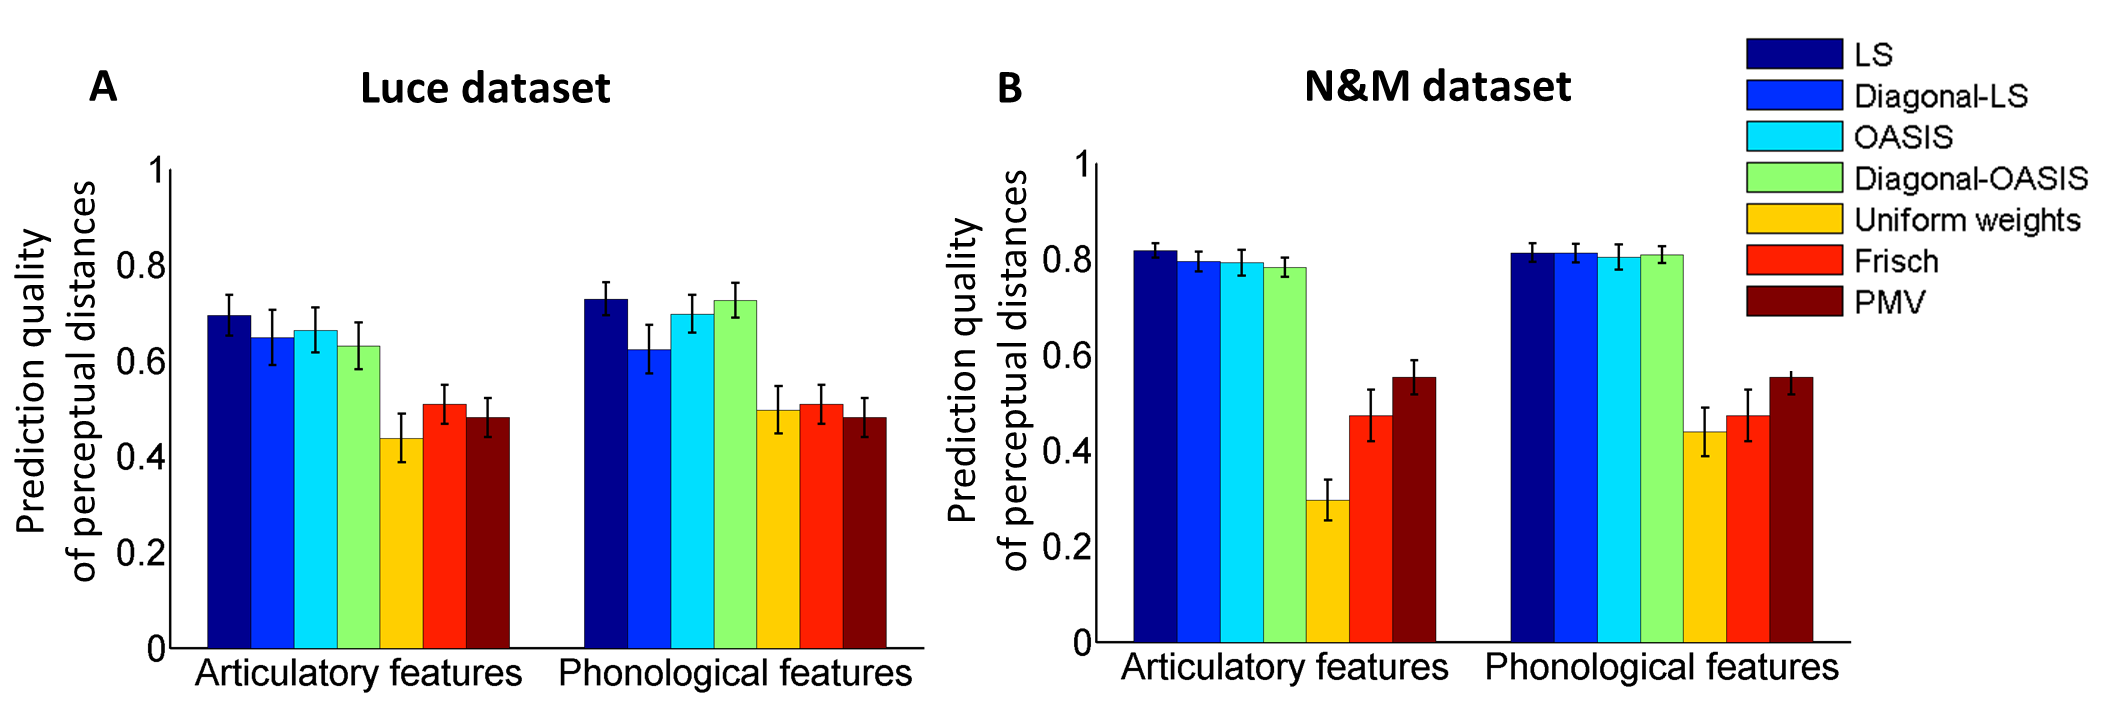
\includegraphics[width=\textwidth]{Figures/Ch2/method_comparison.png}}
\caption{Prediction quality of perceptual distances. For each of the seven methods, the Spearman correlation between the predicted and empirical perceptual distances is calculated, averaged across left-out sets. Error bars represent SD across left-out sets.} 
\end{figure*}

Figure 2.2 compares the average Spearman correlation between the seven methods. Results are shown for both confusion datasets: N\&M dataset, Luce dataset; and for the two feature theories discussed above: articulatory features and phonological features. Model prediction is evaluated in a cross-validation procedure (methods 2.2.5). The prediction of the model is defined as the average Spearman correlation across all validation sets, and the standard deviation is evaluated from the distributions across these sets. To determine the optimal regularizer size model predictions are evaluated on a validation set for various values of the regularization.

Results show that learning feature weights from data significantly improves prediction in comparison to baseline methods (For the N\&M dataset, all comparisons between the data-driven methods and the theoretical measures (Frisch, PMV, uniform weighing) are statistically significant ($p$-value$<10^{-4}$, two-tailed t-test - table 2.3). The four metric-learning methods demonstrate similar predictive power, as tested on these datasets. We therefore select a method for further analysis based on model parsimony and running time. Adding a diagonal constraint results in a more parsimonious model due to its smaller number of free parameters. We therefore choose to use diagonal-LS for the analyses in the rest of this study.

\begin{table}[H]
    \centering
    \begin{tabular}{|c|c|c|c|c|}
        \hline
        \multicolumn{5}{|c|}{Luce - Articulatory features}\\
        \hline
         & LS & Diagonal-LS & OASIS & Diagonal-OASIS \\
         \hline
         Uniform weights & $<10^{-4}$ & $<10^{-4}$ & $<10^{-4}$ & $<10^{-4}$ \\
         Frisch similarity & 0.008 &    0.017 &    0.016 &    0.039 \\
         PMV & 0.003 &    0.034 &    0.006 &    0.031 \\
         \hline
         \multicolumn{5}{|c|}{Luce - Phonological features}\\
         \hline
         & LS & Diagonal-LS & OASIS & Diagonal-OASIS \\
         \hline
         Uniform weights & $<10^{-4}$ &  $<10^{-4}$ & $<10^{-4}$ & $<10^{-4}$ \\
         Frisch similarity & 0.033 &    0.012 &    0.020 &    0.011 \\
         PMV & 0.013 &    0.043 &    0.007 &    0.03 \\
         \hline
         
    \end{tabular}
    \caption{P-values of t-tests for method comparison}
\end{table}


\subsection{Perceptually-discriminative features}
Given the sparsity constraint in the optimization problem (section 2.2.2.1), we interpret the weight of each subphonemic feature as its perceptually discriminative power. We thus examine the resulting weights from each dataset, to see what they reveal about the perceptually properties of the features.

Figure 2.3 shows the learned weights from the N\&M dataset for both the articulatory and phonological-features theories.

\begin{figure*}
\makebox[\textwidth][c]{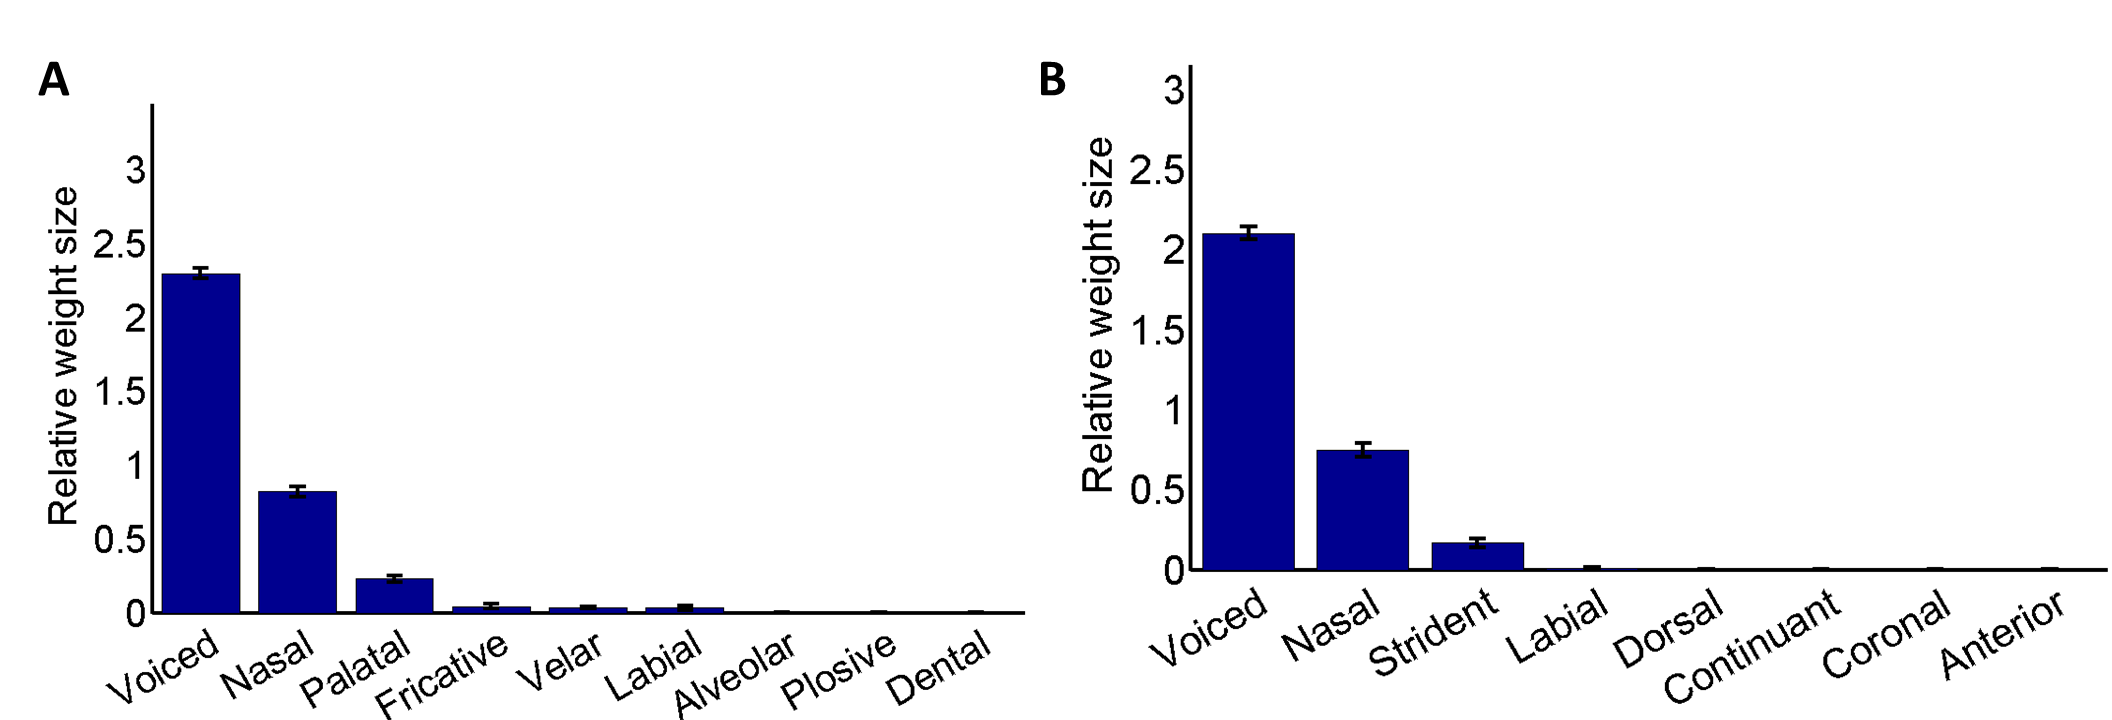
\includegraphics[width=\textwidth]{Figures/Ch2/weight_NM.PNG}}
\caption{Weights of subphonemic features as derived from the Nicely and Miller dataset. (A) Articulatory features (B) Phonological features. Error bars represent SD across validation sets.}
\end{figure*}

\paragraph{Articulatory features} Among the articulatory features, the voicing feature has the highest weight, followed by the nasality feature and then the palatal one. All differences are statistically significant ($p$-value$<10^{-4}$). Next in order are the fricative, velar and labial features, which are statistically comparable. Finally, the alveolar, plosive, and dental features have weights close to zero. Note that similarly to the conclusions from the N\&M study (section 2.3.1), the voicing and nasality features in English are less affected by random noise compared to place features, and other manner features.

\paragraph{Phonological features} When ordered by their weights, the phonological features are: voicing, nasality and the strident feature, in descending order (pairwise differences are statistically significant; t-test $p$-value$<0.05$). The other features, labial, dorsal, continuant, coronal and anterior have weights close to zero. 

Comparing the results of both feature theories, voicing has the highest weight in both cases, which is then consistently followed by nasality. In the third place are the palatal feature for the articulatory theory, and the strident feature for the phonological features theory. Examining this result, we note that the only palatal phonemes in the N\&M dataset are /\textipa{S}/ and /\textipa{Z}/, both are strident consonants. Similarly, when looking into the phonemes that share the strident feature, we find that /\textipa{S}/ and /\textipa{Z}/ are again the only strident phonemes in the N\&M dataset. It therefore seems that a common property of /\textipa{S}/ and /\textipa{Z}/ is the cause for the high weight of these features, and as suggested, it seems that /\textipa{S}/ and /\textipa{Z}/ being stridents, and in particular distributed stridents, is responsible for the result. We therefore summarize the results from the N\&M dataset about the perceptual discrimination of the leading features in the following order: voicing, nasality and distributed-stridents. 

We next examine what the Luce dataset reveals about perceptual-discriminative properties of subphonemic features. Figure 2.4 presents the learned weights from the Luce dataset for both features theories.

\begin{figure*}[h]
\makebox[\textwidth][c]{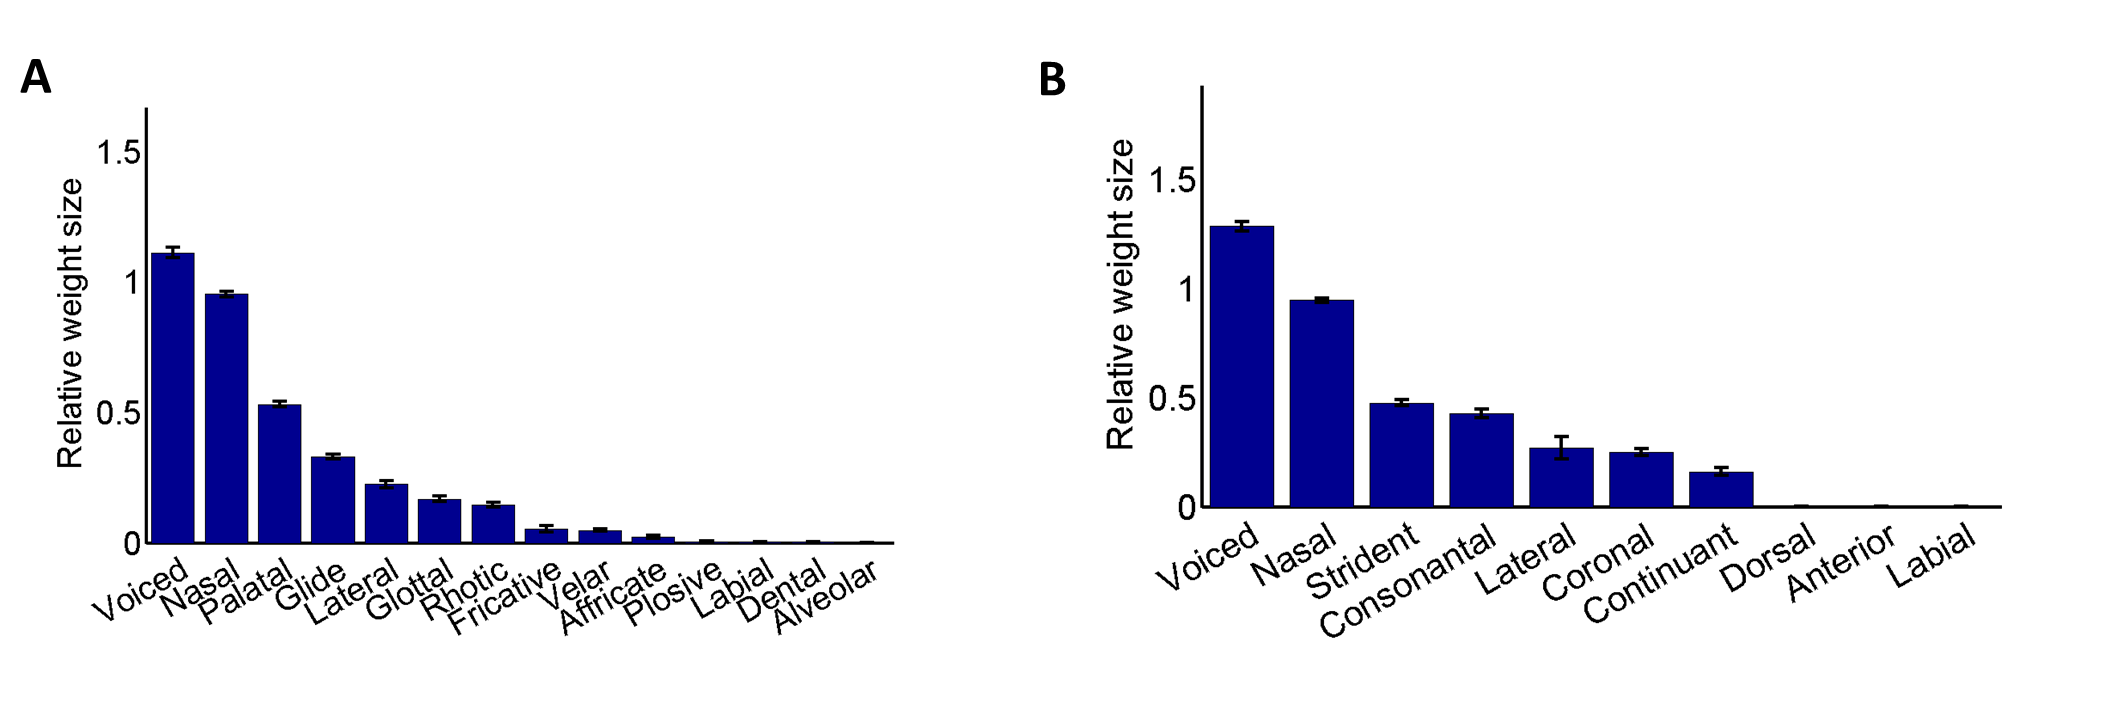
\includegraphics[width=\textwidth]{Figures/Ch2/weight_Luce.PNG}}
\caption{Weights of subphonemic features as derived from the Luce dataset. (A) Articulatory features (B) Phonological features (B). Error bars represent SD across validation sets.}
\end{figure*}



\paragraph{Articulatory features} For the binary representation of articulatory features, the voicing feature has highest weight, followed by nasality, palatal, glide, lateral, glottal and rhotic features, in descending order. All differences are statistically significant (t-test $p$-value$<10^{-4}$) except for the glottal-lateral and glottal-rhotic differences. Next in order are the fricative and velar, which are statistically comparable. The rest of the features - affricate, plosive, labial, dental and alveolar features - have close to zero weights. Similarly to the N\&M dataset, the palatal feature is shared by: /\textipa{S}/, /\textipa{tS}/, and /\textipa{dZ}/, which are all distributed-strident consonants, and also by /\textipa{j}/. As for the glide, lateral, and rhotic features, the corresponding consonant phonemes are /\textipa{w}/ and /\textipa{j}/ (glide phonemes) and /\textipa{l}/ and /\textipa{r}/ (liquid phonemes). These four phonemes are characterized as approximant consonants, as the articulators are closer to each other than for vowels, without creating turbulence in the airflow as is the case with fricative consonants. 

\paragraph{Phonological features} For the phonological features, the resulting order of the subphonemic features is: voicing, nasality, strident, consonantal, lateral, coronal and continuant. All differences are statistically significant (t-test $p$-value$<0.05$) except for the lateral-coronal difference. The other features - dorsal, anterior and labial - have weights close to zero. This order follows a similar pattern to the one described so far: voicing, nasality, distributed-stridents and approximants. The two leading features are again voicing and nasality. The stridency feature, and the consonantal and lateral features, which contrast between the approximant phonemes /j/, /w/ and /l/ to other phonemes, all have relatively high weights also in this case. We therefore summarize the order between subphonemic features, based on all the results so far, as: voicing, nasality, distributed-stridents and approximants. As for the coronal and continuant features, note that they are partially redundant with respect to the leading ones and do not clearly contrast among phoneme sets. For example, the coronal feature is shared by both strident phonemes (/\textipa{s}/, /\textipa{z}/, /\textipa{S}/, /\textipa{tS}/, /\textipa{dZ}/), approximants (/\textipa{l}/, /\textipa{r}/, /\textipa{j}/) and nasal (/\textipa{n}/) phonemes, but also by /\textipa{t}/, /\textipa{d}/, /\textipa{T}/, /\textipa{D}/.

\paragraph{A two-dimensional visualization of perceived distances} To visualize the high-dimensional structure of the perceived distances in the datasets, and the relations between subphonemic features, we use Multi-Dimensional Scaling (MDS) \citep{kruskal1964}, which embeds all perceived distances on the plane. This allows us to qualitatively assess if the learned feature weights are indeed reflected in the visualization of the perceptual distances.

\begin{figure*}[h]
\makebox[\textwidth][c]{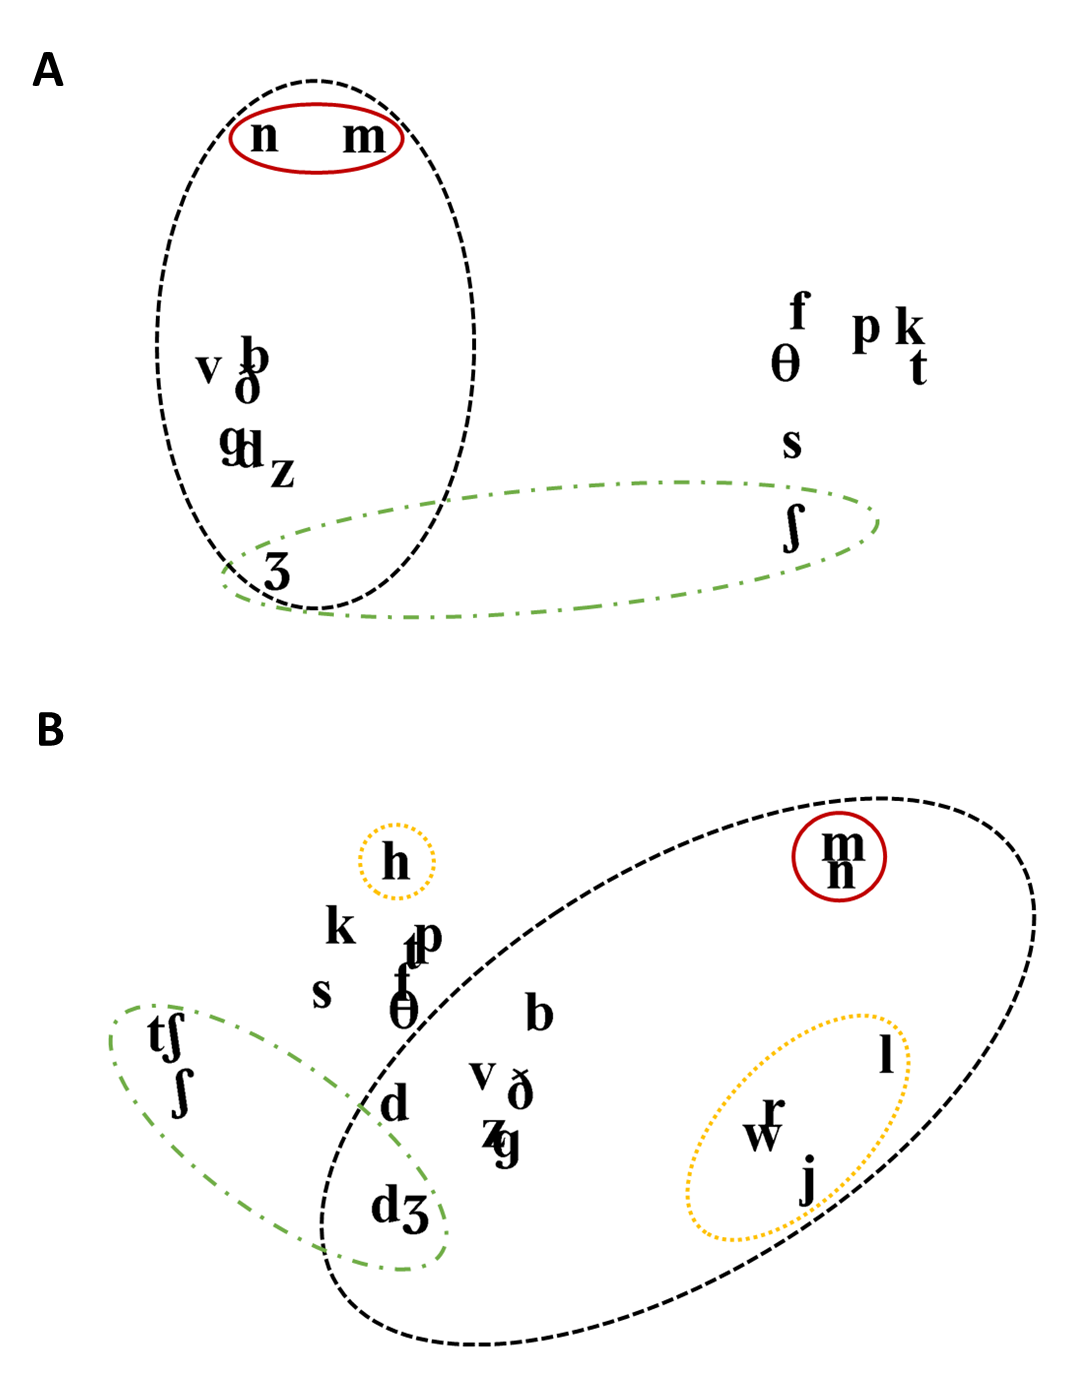
\includegraphics[width=\textwidth]{Figures/Ch2/MDS_english.png}}
\caption{Multi-Dimensional Scaling of perceptual distances between phonemes for the  (A) N\&M datset (B) Luce dataset. Ovals: black (dashed line) - voiced phonemes, red (solid line) - nasals, green - distributed stridents (dash-dot line), yellow (dotted line)- approximants}.
\end{figure*}

MDS is a method for embedding objects and their pairwise distances onto a lower-dimensional space, where the distances between the objects in the lower-dimensional plane approximate the original distances. MDS was already used to explore the N\&M and other phoneme-confusion dataset \citep{Shepard1980, mielke2008emergence, Buchsbaum2015}, we test it also for the Luce dataset. Figure 2.5 presents the results of embedding the perceptual distances between all phonemes into a 2D-plane for the N\&M dataset (panel A) and for the Luce dataset (panel B). The classes of the resulting four leading features are marked with colored ovals: voiced phonemes with black (dashed line), nasal phonemes with red (solid line), distributed-strident phonemes with green (dash-dot line), and approximant-consonants with yellow (dotted line) - the last is only for the Luce dataset, as there were no approximant phonemes in the N\&M experiment. 

The MDS analysis provides several insights. First, for both datasets, voiced and voiceless phonemes reside at opposite sides of the plane. Second, nasal, distributed-strident and approximant phonemes are in the periphery of the plot, and are relatively distant from other phonemes. A phoneme will tend to result in the periphery when it is relatively distant from all other phonemes, which should match a high weight of the corresponding features. Finally, a clear distinction between distributed and non-distributed stridents is observed for both datasets. Among all stridents only the distributed stridents - (/\textipa{S}/, /\textipa{Z}/) in the N\&M dataset, and (/\textipa{tS}/, /\textipa{dZ}/ and /\textipa{S}/) in the Luce dataset - are in the periphery of the plot, whereas the non-distributed stridents (/\textit{s}/, /\textipa{z}/) are more central. This corresponds to the relatively high weights of the palatal feature that is shared by the distributed stridents but not by the non-distributed stridents. To test the variability of the MDS results, we repeated the MDS analysis leaving-out a different phoneme each time - results are qualitatively similar (not shown here).

\paragraph{Redundancy between features} To further examine the resulting feature weights, we tested how omitting a feature from the feature theory would influence the predictive power of the model and the resulting order between subphonemic features. We hypothesized that leaving out features that have relatively high weights would reduce the predictive power of the model and would affect the resulting order.

We therefore repeated the above analyses, leaving out a different feature from the representation scheme on each step, and finally estimating the new prediction of the reduced model. We present results for the larger dataset, the Luce dataset: Figure 2.6 presents the differences between the prediction of the full model and the reduced model, in ascending order of size, for each of the left-out features from the representation scheme. The prediction difference is shown for the two feature theories: articulatory features (panel A) and phonological features (panel B). The prediction difference is significant between the voicing and nasality features compared to all other features (t-test $p$-value$<0.05$), whereas results for the voicing and nasality features are statistically comparable. The palatal feature is statistically comparable to the approximant features - glide, lateral and rhotic features - and to the glottal and fricative features, and significantly different compared to the rest of the features.

\begin{figure}
\vspace{.3in}
\makebox[\textwidth][c]{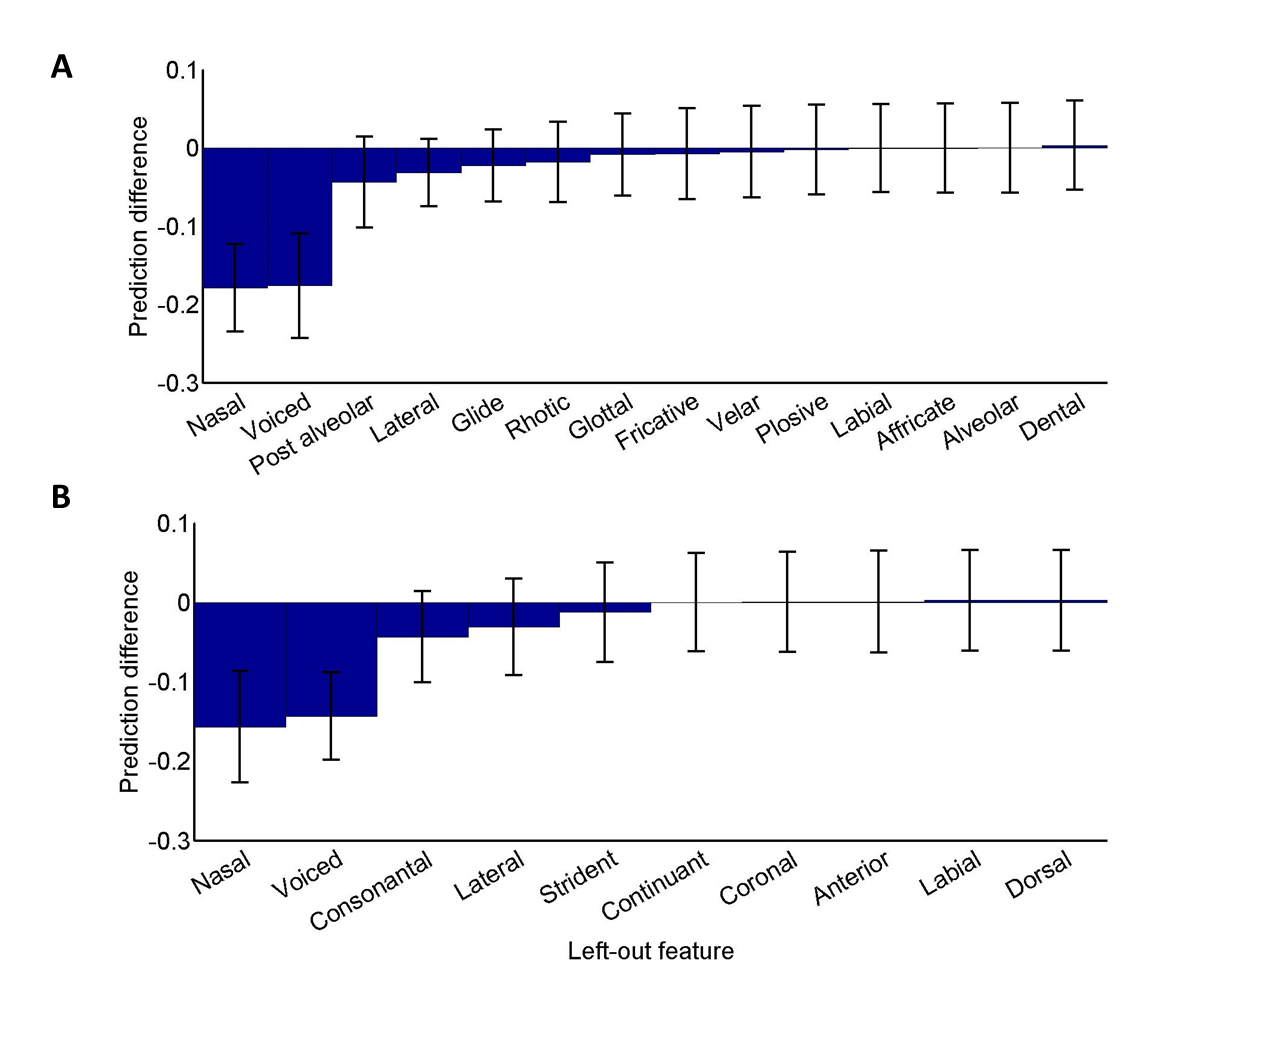
\includegraphics[width=\textwidth]{Figures/Ch2/SWR_prediction.PNG}}
\caption{Reduction in model prediction as a result of omitting a single feature, as calculated for the Luce dataset. (A) Articulatory features (B) Phonological features.}
\end{figure}

Results show that omitting high-weight features significantly reduces the predictive power of the model. In contrast, omitting low-weight features hardly affects prediction.

\subsection{Phoneme confusion in Hebrew and English}
This section analyzes the confusion data of Hebrew in the same way as for English in section 2.4.2. Hebrew phonemes are represented based on two feature theories as described above, and the LS-diagonal method is applied for each of these cases.

\begin{figure*}[h]
\vspace{.3in}
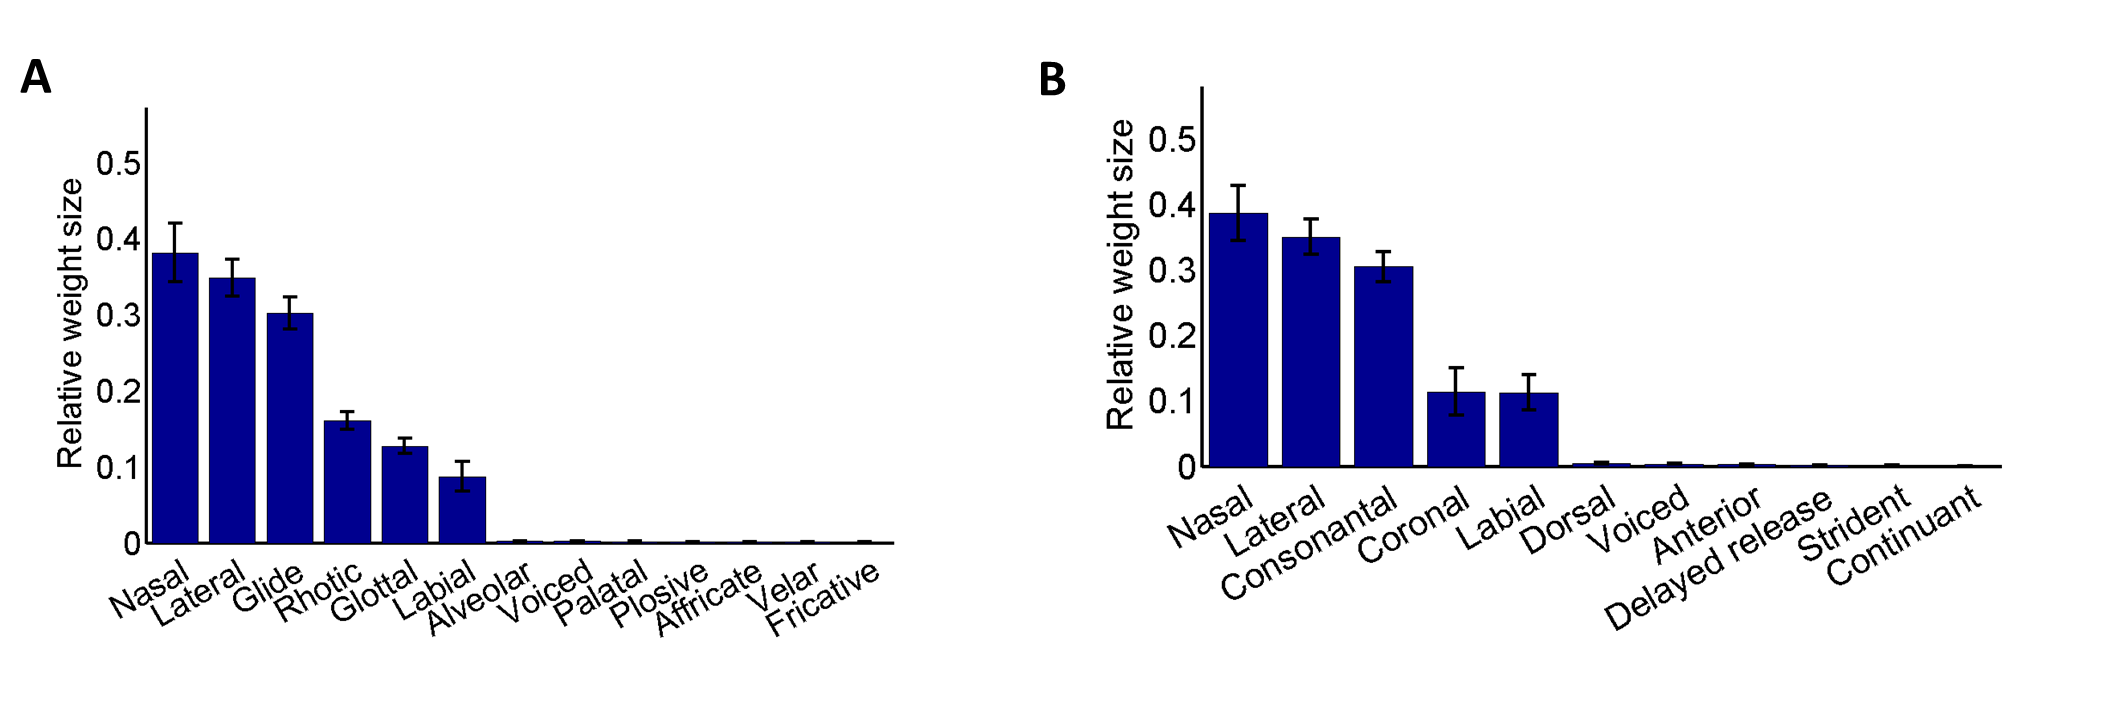
\includegraphics[width=\linewidth]{Figures/Ch2/weight_Heb.PNG}
\caption{Weights of subphonemic features as derived from the Hebrew dataset. (A) Articulatory features (B) Phonological features. Error bars represent SD across validation sets.}
\end{figure*}

Figure 2.7 shows the resulting feature weights for articulatoy and phonological features. Computed for the Hebrew dataset, results show that as in English datasets, the nasality feature and the approximant features - lateral, glide and rhotic - are heavily weighted. The voicing feature, on the other hand, has much lower weight in Hebrew compared to English. In addition, the labial feature in both articulatory and phonological feature theories has relatively high weight compared to the English results.

The results of MDS analysis on the Hebrew dataset (Figure 2.8A) agree with the results of the metric learning. Nasal phonemes are embedded in the periphery of the plot, as well as the approximants and the glottal phoneme /h/. Unlike the N\&M and Luce embeddings, voiced phonemes are not well separated from unvoiced phonemes. The locations of the labial phonemes /p/ and /f/ in the MDS analysis is peripheral, which corresponds to the relatively high weight of the labial phoneme. 

\begin{figure}
\vspace{.3in}
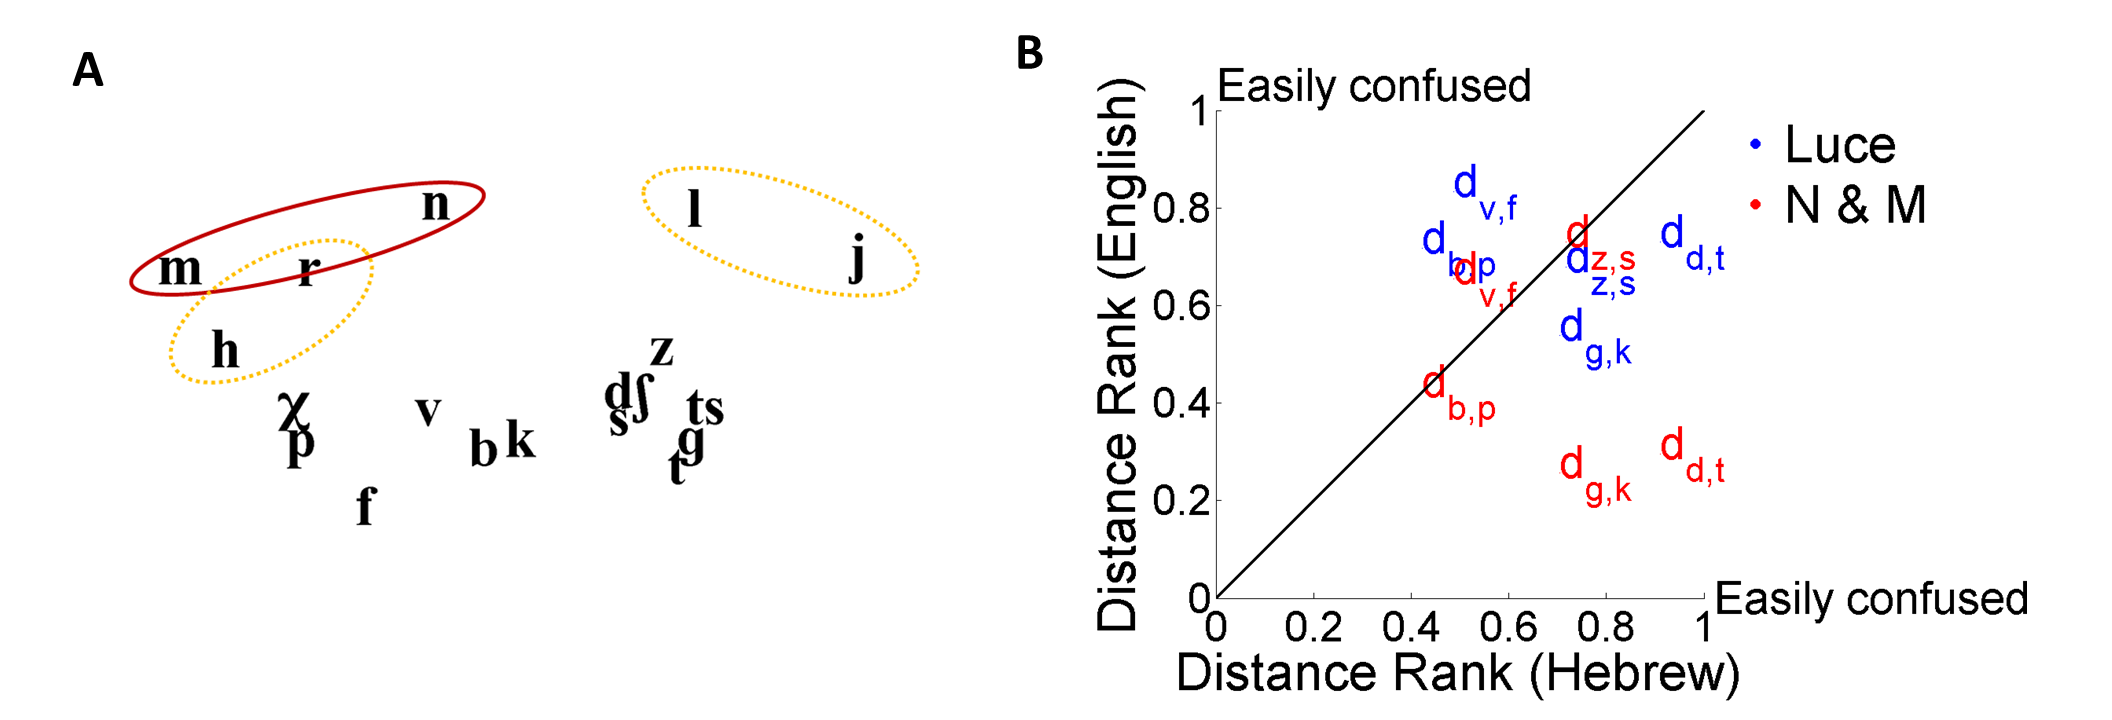
\includegraphics[width=\linewidth]{Figures/Ch2/Slide5.PNG}
\caption{(A) Multi-Dimensional Scaling for the Hebrew dataset. Ovals: red (solid line) - nasals, yellow (dotted line)- approximants and the glottal /h/(B) Voicing-differing minimal pairs: Hebrew vs. English}
\end{figure}

Figure 2.8B summarizes the differences between the Luce dataset and Hebrew with respect to perceptually-discriminative power of subphonemic features. Values on each axis represent normalized weights. Subphonmeic features that are below the line $y = x$ are more perceptually discriminative in Hebrew, and vice versa. Note that the farthest feature from the line is the voicing feature. Given this large discrepancy with respect to voicing between English and Hebrew, we further analyze this difference in the following subsection.

\subsubsection{Voicing-differing minimal pairs} To further examine the difference between Hebrew and English with respect to voicing, we compare a set of minimal pairs that only differ in voicing. We extract perceived pairwise distances between (/b/-/p/, /d/-/t/, /g/-/k/, /z/-/s/ and /v/-/f/) from the three datasets, and compare their rank on a scatter plot (figure 2.9). Ranking is necessary to equalize the distributions across languages: the values on the axes represent the rank of the perceived distance of a pair among all other pairwise distances. Before ranking distances, the largest subset of phonemes shared by all three datasets (13 phonemes) was first extracted. This was done to ensure that the rank of the distance does not depend on the specific phoneme inventory of the dataset. Features that corresponds to points above the line $y=x$ are more confusable in Hebrew than in English, and vice versa. The distance of a point from this line can serve as a measure of the difference between the two languages, with respect to the voicing difference between the phonemes in the minimal pair.

There are ten pairwise distances, five for the contrast between Hebrew and the Luce dataset (blue), and five for the contrast between Hebrew and the N\&M dataset (red). Among the ten points, five points are below the dividing line, three points above, and two reside on the line. There is a bias towards more confusion in Hebrew compared to English, with respect to voiced/voiceless phoneme confusion. This agrees with the relatively low weight of voicing in Hebrew. However, looking at the distribution of distances from the dividing line, this bias is not statistically significant (Wilcoxon rank test $p$-value$=0.57$). A possible confounding for this is the relatively high weight of the labial feature in Hebrew, in particular, the relatively large distance of /p/ and /f/ from other phonemes as can be observed in the MDS analysis. This could counteract the difference between English and Hebrew with respect to voicing. Looking at the distribution of the non-labial phonemes (/d/-/t/, /g/-/k/ and /s/-/z/) the bias towards Hebrew is significant (Wilcoxon rank test $p$-value$<0.05$).

\begin{figure}
\vspace{.3in}
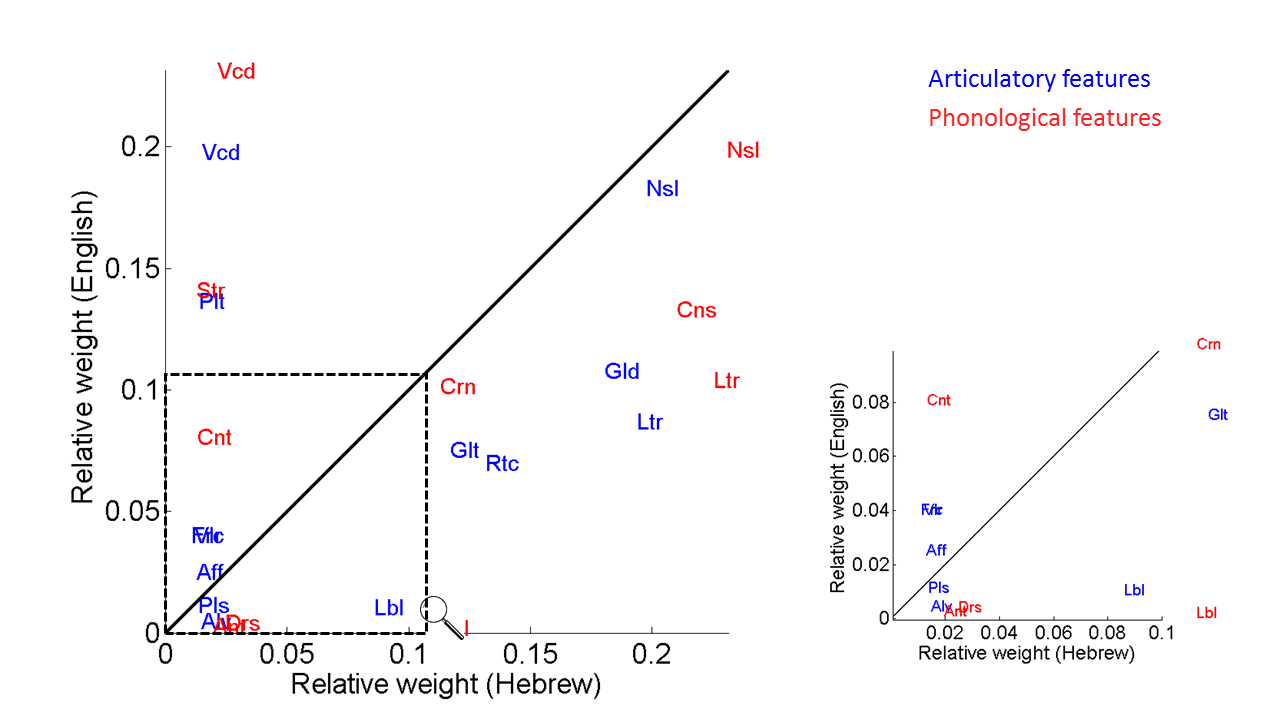
\includegraphics[width=\linewidth]{Figures/Ch2/compare_Heb_Luce.PNG}
\caption{English vs. Hebrew: relative weights of features. Articulatory features in blue, Phonological features in red. Dashed square indicates the magnified area (bottom-right). Features that corresponds to points above the line $y=x$ are more confusable in Hebrew than in English, and vice versa. Feature names are abbreviated according to their three first consonants in their name.}
\end{figure}
\section{Summary and Discussion}
This study explores a new framework to the problem of phoneme similarity. Using learning algorithms, it derives a feature-based metric function from phoneme-confusion data. In doing so, it provides means to quantify the contribution of subphonemic features to the overall similarity. Moreover, since feature weights compete among themselves over explaining empirical perceptual distances (Appendix B), the resulting weights are interpreted as perceptually saliencies of features.

The study relies on several simplifying assumptions that can be alleviated in future studies: for computational convenience, it assumes a linear mapping between the feature and similarity spaces. However, the suggested framework provides freedom in the choice of the abstract form of the metric function, which, in general, can incorporate any type of non-linearity (Eq. 2.1). Second, the study assumes that perceptual similarities are symmetric, despite accumulating opposing evidence. However, asymmetric metrics, namely - quasimetrics, can be learned using the same approach. Once the form of the quasimetric is chosen, its parameters can be learned from the data, in the same way, subject to minor modifications of the learning algorithms. 

We explored with two classic phoneme-confusion datasets in English \citep{NicelyMiller1955, Luce1987} and two common feature theories (\citealp{ChomskyHalle1968}, and articulatory dimensions). We then derived a metric function for each dataset and feature theory, and described the resulting order among subphonemic features with respect to their perceptual saliencies. The four leading groups of subphonemic features in English, in descending order, are: voicing, nasality, distributed-stridents, and approximants. Favorably, this is in accordance with previous studies and acoustic considerations: the voicing and nasality features have been demonstrated as highly perceptually discriminating using information-theory measures \citep{NicelyMiller1955}. As for distributed-stridents, this class of phonemes have relatively high energy in their waveform, which may explain their relatively high weight. Acoustic analyses conducted by \citep[see][Figure 15]{Mielke2012} showed that stridents are distinguished from other phonemes along the first principal component of acoustic distances, which is interpreted as dominance of high-frequency acoustic energy. However, a distinction between distributed stridents and non-distributed stridents was not observed in this analysis. The second principal component of this analysis, which is interpreted as dominance of low-frequency acoustic energy, distinguishes the nasal and approximant phonemes /n/, /m/, /w/, /j/, /l/, /r/ and /h/ from the other phonemes in the datasets, in this order. This shows that the relatively high weight of approximant features and the fricative glottal /h/ is also grounded in acoustics.

Confusion-rate results among Hebrew phonemes were reported. The new Hebrew dataset was analyzed and compared to the English ones, revealing a discrepancy between Hebrew and English with respect to subphonemic feature weights. In particular, a major difference with respect to voicing was found. We suggest two possible sources for this difference. First, it can be accounted for by redundant cues for unvoiced plosives in English that are absent in Hebrew. A redundant cue is an articulatory-independent mechanism to enhance a primary cue in the signal. In particular, \citet{stevens1989primary} suggests that the feature [-voice] is enhanced by glottal opening (aspiration) in English, which prolongs the duration of the voiceless interval, thus rendering voiceless stops more distinguishable from voiced stops. Hebrew and other languages (e.g., French) do not employ this enhancement. Another explanation for the different weight of voicing is the differences in voicing onset times (VOT) \citep{Laufer1998} between the two languages. VOTs of voiced stops in Hebrew are more negative than in English, which may affect perceptual discrimination.  Taken together, this result is another evidence that the metric space may
differ across languages.


In sum, this study is a first demonstration of the benefits of a data-driven approach to the problem of phoneme similarity. Its general framework was shown to have several potential advantages, and provides means to quantify various aspects of phoneme similarity.
{\normalfont%
    \huge% %change this size to your needs for the first line
    \bfseries}{\chaptertitlename\ \thechapter}{20pt}{%
    \Huge %change this size to your needs for the second line
    }

\titleformat{\chapter}[display]
{\normalfont%
    \Large% %change this size to your needs for the first line
    \bfseries}{}{20pt}{%
    \LARGE %change this size to your needs for the second line
    }
%% Chapter 3
\lhead{\emph{Chapter 3: The Functional Organization of Phonemes in the Superior Temporal Gyrus (STG) as Revealed by Spiking Activity}}
\chapter{Chapter 3: The Functional Organization of Phonemes in the Superior Temporal Gyrus (STG) as Revealed by Spiking Activity}

\section{Introduction}
A long lasting controversy persists in psycholinguistic research regarding the involvement of the motor system in speech perception. The motor theory of speech perception describes phoneme perception in terms of the articulatory gestures that generate it. According to this theory, the objects of speech perception are the intended phonetic gestures of the speaker, such as, ‘lip rounding’, or ‘jaw raising’ \citep{liberman1967perception, liberman1985motor}. For example, [m] consists of a labial stop gesture combined with a velum-lowering gesture. On the other hand, auditory theories argue that phonetic processing depends directly on properties of the auditory system \citep{jakobson1951preliminaries, stevens1972quantal, stevens1989quantal, stevens2002toward}. According to this view, listeners identify spectrotemporal patterns in the phoneme waveforms and match them to stored acoustic representations. For example, vowels are characterized by a roughly bimodal spectra and sibilant fricatives by high-frequency energy.


The fundamental motivation of the motor theory arose from an early observation that phoneme percepts are invariant across different contexts \citep{cooper1952some, liberman1967perception}. In the case of coarticulation, several gestures overlap in time, which may cause the acoustic waveform of the same intended gesture to be significantly different than when it is pronounced in isolation. Therefore, a particular gesture can be represented by different acoustic waveforms in different phonetic contexts. Additional variation exists in the acoustic signal due to inter-speaker variability.  This considerable variability led the supporters of the motor theory to propose that the objects of speech perception are not to be found in acoustics.

Phoneme perception has been the focus of many neuroimaging studies \citep{liebenthal2005neural, dehaene2005neural, mottonen2006perceiving, desai2008left, liebenthal2010specialization,  formisano2008saying, binder2000human, Dewitt2012}. One common method in these studies uses sophisticated baselines to speech, such as rotated speech, to elicit activation in regions that are selective to speech, but not to nonphonemic contrasts.  The results describe a complex picture of hierarchically-organized phoneme processing in the temporal lobe, from primary auditory and early posterior auditory areas to higher-level processing in the anterior, ventral STG and STS. 

Invasive electrophysiological recordings in humans provide a precious glimpse into the neural representations of linguistic entities, such as the objects of speech perception, with high temporal resolution and spatial localization compared to non-invasive recording techniques. Several recent studies, using Electrocorticography (ECoG) grids, have contributed to our understanding of neural encoding in higher-level auditory cortex, and shed new light on the long-lasting debate in speech perception. \citet{pasley2012reconstructing} showed that speech waveforms can be reconstructed from neural activity in the lateral STG, suggesting that encoded information in this region is mainly acoustic. More recently, \citet{Mesgarani2014} have characterized the functional organization of phonemes in the peri-Sylvian speech cortex. The study provides a detailed examination of neural representations of phonemes in the STG of human subjects, during listening to natural speech. Examining the functional organization in this region, they found that phoneme representations cluster according to acoustic features, in an hierarchical manner. Remarkably, the dominant organizing acoustic features are the same distinctive features defined by linguists half a century ago \citep{ChomskyHalle1968}. Moreover, an order was found among the features: manner-of-articulation features produce a neural invariance that is more prominent than that related to place-of-articulation (more recently, a similar order was found also using EEG recordings \citep{khalighinejad2017dynamic}). This order is consistent with an early observations from language acquisition, according to which manner-of-articulation distinctions are acquired early during childhood, compared to the place-of-articulation ones \citep{jakobson1968child, grodzinsky2014neural}. Taken together, these findings support the auditory view of speech perception rather than gestural theories. Other ECoG studies have further examined the functional organization of phonemes outside the STG, and tested its dependency on the experimental task (listening vs. production). Results show that the organization can significantly differ across brain regions and tasks: \citet{bouchard2013functional} showed that the functional organization of phonemes in the vSMC during production is dominated by place-of-articulation features (e.g., labial, alveolar, velar and glottal), in contrast to manner-of-articulation features in the STG during listening. More recently, the functional organization in the same region was found to differ also across tasks. Whereas during phoneme production, the dominant organizing feature of neural activity in the vSMC is place-of-articulation, during listening, the organization in the same region was found to be dominated by manner features, similarly to the STG \citep{cheung2016auditory}.

ECoG studies have greatly enriched our understanding of the neural basis of speech perception.  However, the electrical activity recorded in ECoG grids reflects average responses of large neuronal populations, as non-invasive methods, and is therefore limited in providing insights into activity patterns of single cells. Describing and construing single-cells activity is indispensable for a complete theory of the neural basis of speech perception, and cognitive processes in general. Single-unit recording was pioneered at the mid of the previous century, and was later developed to obtain multiple single-unit recordings from deep brain structures in humans \citep{fried1999cerebral} (for a review, \citealp{engel2005invasive, mukamel2012human, cash2015emergence}). It provides unique spatiotemporal resolution and valuable information about processes that are unique to humans, such as language \citep{heit1988neural, creutzfeldt1989neuronal, tankus2012structured, ossmy2015decoding}.

Consistent with findings from ECoG and EEG studies, single-cell studies on phonetic processing revealed a multidimensional neural representation of phonemes by demonstrating that STG neurons are tuned to subsets of phonemes and have a sparse coding scheme \citep{creutzfeldt1989neuronal, chan2013speech}. However, the functional organization of phonemes at the cellular level is still poorly understood. Specifically, whether single STG neurons encode phonemes in an hierarchical way, as was revealed by analyzing gamma activity in ECoG studies, with larger invariance to manner- compared to place-of-articulation features.

In this study, we recorded spiking activity from the superior temporal gyrus of six neurosurgical patients while they listened to simple speech stimuli in the form of consonant-vowel (CV) pairs, generated by three speakers. We characterized STG single-cell responses to the stimuli, and examined the functional organization of phonemes as revealed by single-cells activity. In particular, we addressed the question about the dominating organizing dimension, by quantifying manner- and place-of-articulation invariances, using probabilistic modelling.

The study also examines the relation between the functional organization of phonemes as revealed by single-cells activity, and the cognitive one as estimated from behavioral data. We collected phoneme-confusion rates from normal subject, using the same set of stimuli as in the experiment with neurosurgical patients. We then quantified the extent to which the cognitive and neural functional organizations correspond. 

\section{Materials and methods}
\subsection{Patients and electrophysiological recording}
Data was collected from six patients with pharmacologically intractable epilepsy, implanted with intracranial depth electrodes to identify seizure focus for potential surgical treatment \citep{mukamel2012human}. Electrode location was based solely on clinical criteria. Each electrode terminated in a set of nine 40-$\mu$m platinum–iridium microwires \citep{fried1999cerebral} — eight active recording wires, referenced to the ninth. Signals from these microwires were recorded at 40 kHz using a 64-channel acquisition system. Before surgery each patient underwent placement of a stereotactic headframe, and then a detailed MR image was obtained using a spoiled-gradient sequence, followed by cerebral angiography. Both anatomical and angiography images were transmitted to a workstation in the operating room, and surgical planning was then performed, with selection of appropriate temporal and extra-temporal targets and appropriate trajectories based on clinical criteria. To verify electrode position, CT scans following electrode implantation were co-registered to the preoperative MRI using Vitrea® (Vital Images Inc.). The patients provided written informed consent to participate in the experiments. The study was approved by and conformed to the guidelines of the Medical Institutional Review Board at UCLA and Ichilov.

\subsection{Stimuli and behavioral task}
Stimuli were constructed of either consonant-vowel (CV) pairs, or vowels /aeiou/ presented in isolation. The consonants in the CV syllables were according to the list in Table A.1, and the vowel was set to /a/ in order to reduce effects on the preceding consonant. To increase data size, we collected recordings from both Hebrew- and English-speaking patients. We therefore focused on a phoneme set that is approximately shared for both languages. Patients  were presented with 12 repetitions from each CV pair or vowel, 4 from each speaker, in a random order (ISI = 1 second). The patients were instructed to listen carefully to the syllables.


\begin{landscape}% Landscape page
\begin{table}[H]
\centering % Center table
\tiny
\begin{tabular}{|c|c|c|c|c|c|c|c|c|c|c|c|c|c|c|c|c|c|c|c|c|c|c|c|c|c|}
\hline

&\multicolumn{21}{|c|}{Features}\\
\hline
&	a	&	e	&	o	&	i	&	u	&	n	&	m	&	l	&	j	&	f	&	v	&	s	&	z   & \textipa{S}	&	\textipa{Z}	&	p	&	b	&	t	&	d	&	k	&	g	\\
\hline

$sonorant$	&	+	&	+	&	+	&	+	&	+	&	+	&	+	&	+	&	+	&	-	&	-	&	-	&	-	&	-	&	-	&	-	&	-	&	-	&	-	&	-	&	-	\\
$vowel$	&	+	&	+	&	+	&	+	&	+	&	-	&	-	&	-	&	-	&	-	&	-	&	-	&	-	&	-	&	-	&	-	&	-	&	-	&	-	&	-	&	-	\\
$nasal$	&	-	&	-	&	-	&	-	&	-	&	+	&	+	&	-	&	-	&	-	&	-	&	-	&	-	&	-	&	-	&	-	&	-	&	-	&	-	&	-	&	-	\\
$approximant$	&	-	&	-	&	-	&	-	&	-	&	-	&	-	&	+	&	+	&	-	&	-	&	-	&	-	&	-	&	-	&	-	&	-	&	-	&	-	&	-	&	-	\\
$fricative$	&	-	&	-	&	-	&	-	&	-	&	-	&	-	&	-	&	-	&	+	&	+	&	+	&	+	&	+	&	+	&	-	&	-	&	-	&	-	&	-	&	-	\\
$plosive$	&	-	&	-	&	-	&	-	&	-	&	-	&	-	&	-	&	-	&	-	&	-	&	-	&	-	&	-	&	-	&	+	&	+	&	+	&	+	&	+	&	+	\\
labial	&	-	&	-	&	-	&	-	&	-	&	-	&	+	&	-	&	-	&	+	&	+	&	-	&	-	&	-	&	-	&	+	&	+	&	-	&	-	&	-	&	-	\\
coronal	&	-	&	-	&	-	&	-	&	-	&	-	&	-	&	+	&	-	&	-	&	-	&	+	&	+	&	+	&	+	&	-	&	-	&	+	&	+	&	-	&	-	\\
dorsal	&	-	&	-	&	-	&	-	&	-	&	-	&	-	&	-	&	+	&	-	&	-	&	-	&	-	&	-	&	-	&	-	&	-	&	-	&	-	&	+	&	+	\\
alveolar	&	-	&	-	&	-	&	-	&	-	&	+	&	-	&	+	&	-	&	-	&	-	&	+	&	+	&	-	&	-	&	-	&	-	&	+	&	+	&	-	&	-	\\
palatal	&	-	&	-	&	-	&	-	&	-	&	-	&	-	&	-	&	+	&	-	&	-	&	-	&	-	&	+	&	+	&	-	&	-	&	-	&	-	&	-	&	-	\\
velar	&	-	&	-	&	-	&	-	&	-	&	-	&	-	&	-	&	-	&	-	&	-	&	-	&	-	&	-	&	-	&	-	&	-	&	-	&	-	&	+	&	+	\\
\hline

\end{tabular}
\caption{List of consonant and vowels in the experiment}
\end{table}
\end{landscape}

All stimuli were recorded in an anechoic chamber with a RØDE NT2-A microphone and a Metric Halo MIO2882 audio interface, at a sampling rate of 44.1kHz. Stimuli were generated by two male and one female speakers. The total number of stimuli was 63 (21 phonemes * 3 speakers). Length and pitch (by semi-tone intervals) were compared across recorded tokens to choose the most highly comparable stimulus-types. This was done by looking at differences in timeline arrangement, using built-in pitch tracker in a commercial software (\textit{Logic Pro X}). Further cleaning of noise residues in high resolution mode was done, applying extremely mild reduction levels (using \textit{Waves X-Noise} software).

\subsection{Data Preprocessing}
To detect spiking activity, the data was band-pass filtered offline between 300 and 3000 Hz and spike sorting was performed using WaveClus \citep{quiroga2004unsupervised}, similar to previous publications \citep{quiroga2005invariant}. This process yields for each detected neuron a vector of time stamps (1 ms resolution) during which spikes occurred. To assess responsiveness of each neuron to the phonemes we compared speech to non-speech response. For this, we computed a t-test between the spike-count distribution before stimulus onset (-500-0ms) and after (0-500ms). Neurons with statistically-significant responses ($p-value<0.05$) were included in subsequent analyses. 

\subsection{Optimal integration window}
The time lag from stimulus onset may be crucial for the analysis. A time window that is too early or too late with respect to stimulus onset, may not capture the information encoded by the neuron. Therefore, we first identified a time window for each patient and unit, in which the neural representations of different phonemes are most separable. We estimated separability by calculating the between-class to within-class variability ratio of the spike-count in the specific time window (F-statistic). We calculated the F-statistic for all time lags (0-500ms) with respect to the phoneme onset, using a running time window of 200ms duration. We determined the optimal integration window according to the maximal F-statistic, centered to the time for which it was maximal (Figure A.1). The size of the time window was chosen similarly to previous single-unit studies \citep{cash2015emergence}, and based on a qualitative assessment, small changes (100-300ms) did not have a significant effect on the rest of the results. Finally, to capture the dynamics of the neural response, the optimal time window was binned into small bins of 50ms (e.g., \citealp{Mesgarani2014}). 
\begin{figure}[H]
\vspace{.3in}
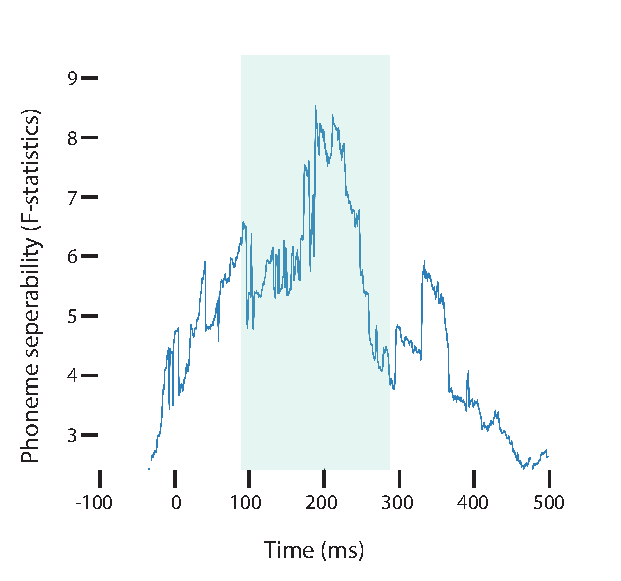
\includegraphics[width=\linewidth]{Figures/Ch3/Figure1_new.eps}
\caption{Optimal integration window: F-statistic for a running window of 200ms, averaged across units. Time values represent the center of the time window. We determined the optimal integration window (shaded area) according to the peak.}
\end{figure}

\subsection{Naive Bayes Classifier}
We model the observed spike counts from all units assuming the generation process of spikes follows a Poisson distribution. Formally, the probability of observing $k$ spikes in a time bin, generated by unit $i$ in response to the presentation of stimulus type $s$, is:

\begin{equation}
    p(k \  spikes \ in  \  response  \  to  \  stimulus  \  type \  s)=e^{-\lambda_{i,s}}\frac{\lambda_{i,s}^k}{k!}
\end{equation}

Where, $\lambda_{i,s}$ is the firing rate of unit $i$ in response to stimulus type $s$. Given a stimulus type (e.g., a phoneme or a phonological feature), we further model the joint spike activity across units, using a Naive Bayes model. We assume that the observed spike counts across units are independent of each other, enabling a simple factorization of the joint probability of stimulus and responses. Formally, the probability of observing a spike-count pattern $x \in \mathbb{R}^n$ across units in response to the presentation of a stimulus type $s$ is:

\begin{equation}
    p(x|s)=\prod_{i=1}^n{p(x_i |s)}=\prod_{i=1}^n{e^{-\lambda_{i,s}}\frac{\lambda_{i,s}^k}{k!}}
\end{equation}

Where, $n$ is the number of units. For each classification task, we split the data into training and test sets, keeping the number of labels in the test set equal across classes. First, we estimate the firing-rate parameters $\lambda_{i,s}$ from the training data using maximum likelihood. That is, for each stimulus type s and unit i, we find the firing-rate parameter $\lambda_{i,s}$ that maximizes the likelihood of observing the spike counts in the training-set trials: $\prod_{t \in training-set}{e^{-\lambda_{i,s}}\frac{\lambda_{i,s}^k}{k!}}$. Then, having estimated all firing-rate parameters, and given the observed activity pattern x across all units, we infer for each trial in the test-set the most probable stimulus type $s$ given the observed activity pattern $x$ across all units. Using Bayes rule, the posterior distribution is:

\begin{equation}
    p(s|x) \propto p(x|s)p(s) = \prod_{i=1}^n{e^{-\lambda_{i,s}}\frac{\lambda_{i,s}^k}{k!}p(s)}
\end{equation}

Where, $p(s)$ is the prior probability of the stimulus type, which was set as uniform.

The mode of the posterior distribution indicates the most probable stimulus type given the firing pattern across units. This can be used for calculations of classification accuracies of the stimulus types. However, the full posterior distribution provides additional information about the similarity structure among the stimulus types. Therefore, for each stimulus type we generate the average posterior distribution across all trials in the test set. Next, for each classification task we construct a confusion matrix, in which each row represents the average posterior distribution for a given stimulus type. In addition, we calculate classification accuracies for various phonological features, comparing the mode of the posterior distribution and the ground-truth label (see Section 3.3.2). We use a 5-fold cross-validation procedure - the mean firing rates for each unit and condition are learned from a training set and classification accuracies are evaluated from the unseen test sets. Finally, statistical significance is determined from the distribution of accuracy values across test sets.


\subsection{A comparison between neural and behavioral data}
To test whether phonemes similarity at the behavioral level corresponds with population spiking activity in single STG neurons, we generated two phoneme-similarity matrices - a behavioral and a neural one. The former is generated from phoneme confusability according to: $S_{ij}=\frac{p_{ij}+p_{ji}}{p_{ii}+p_{jj}}$, where $p_{ij}$ is the probability of confusing phoneme $i$ with phoneme $j$ (section 2.2.2). The latter is based on neural activity in the following way: first, we calculated the standard score (z-score) of the spike-count activity in the optimal integration window. Next, for each pair of phonemes $i$ and $j$, we calculated the Euclidean distance $d_{ij}$, and then the phoneme similarity according to the following (monotonic) function: $S_{ij}=exp(-d_{ij})$. Finally, we performed Spearman rank correlation between the two matrices. The result is therefore not affected by the exact shape of the function. 

\section{Results}
We recorded neural activity from six patients, implanted with intracranial depth electrodes, during a listening task in which auditory stimuli of various phonemes were presented. We describe the representation of phonemes at the single-neuron level, and explore their functional organization with respect to phonological features. In particular, in section 3.3.2 we examine whether the functional organization is more dominated by place-of-articulation or by manner-of-articulation features. Section 3.3.3 compares the similarity structure of phoneme representations as revealed by population spiking activity and that derived from a behavioral experiment, using the same set of stimuli in both experiments.


\subsection{Spike sorting and tuning curves}
Units were sorted using WaveClus and assessed for responsiveness to phoneme stimuli (section 3.2.3). Figure 3.1 presents an example of raster and PSTH plots from one STG unit from one patient. Consonanta are grouped according to plosives, fricatives and nasal-approximant (Panels A-C); Vowels are embedded in approximant locations in formant space (Panel D).

\begin{figure}[H]
\vspace{.3in}
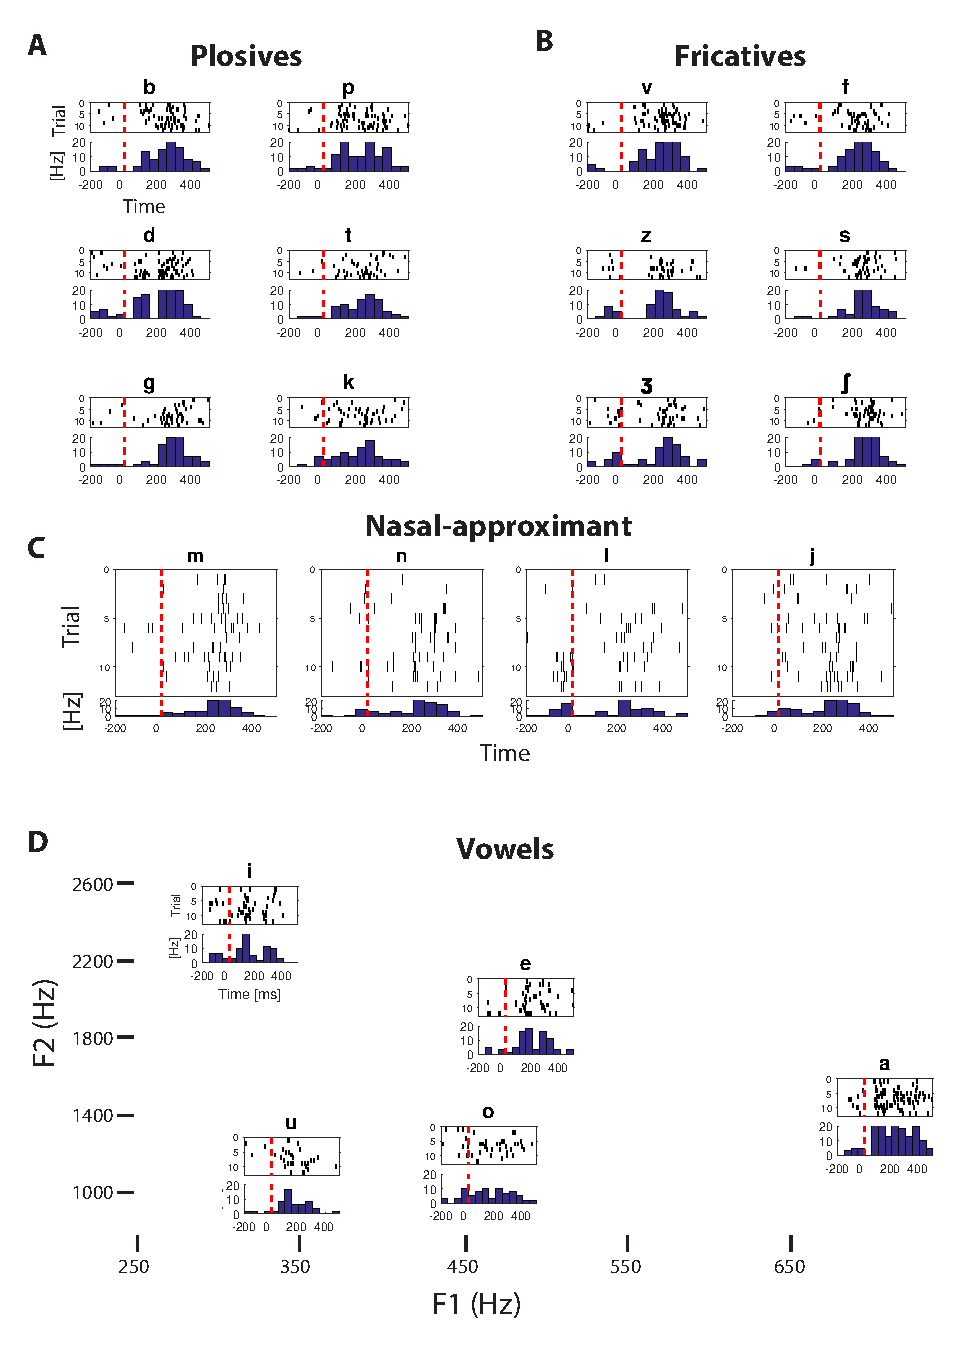
\includegraphics[width=\linewidth]{Figures/Ch3/Figure2_new.eps}
\caption{Raster and PSTH plots for an example unit, from one of the patients. (A) Voiced (left) and unvoiced (right) plosives (B) voiced (left) and unvoiced (right) fricatives (C)  nasal-approximant (left) and affricate (right) phoneme (D) Vowel rasters are embedded in approximant locations in the formant space}
\end{figure}

We describe the average responses of the fourteen selected units to all phonemes in the experiment. For each phoneme, we plot the mean firing rate in an optimal integration window (section 3.2.4), for which phoneme separability is maximal. Figure 3.2 presents mean spike-count activity in the optimal time window, for all units.

\begin{figure}[H]
\vspace{.3in}
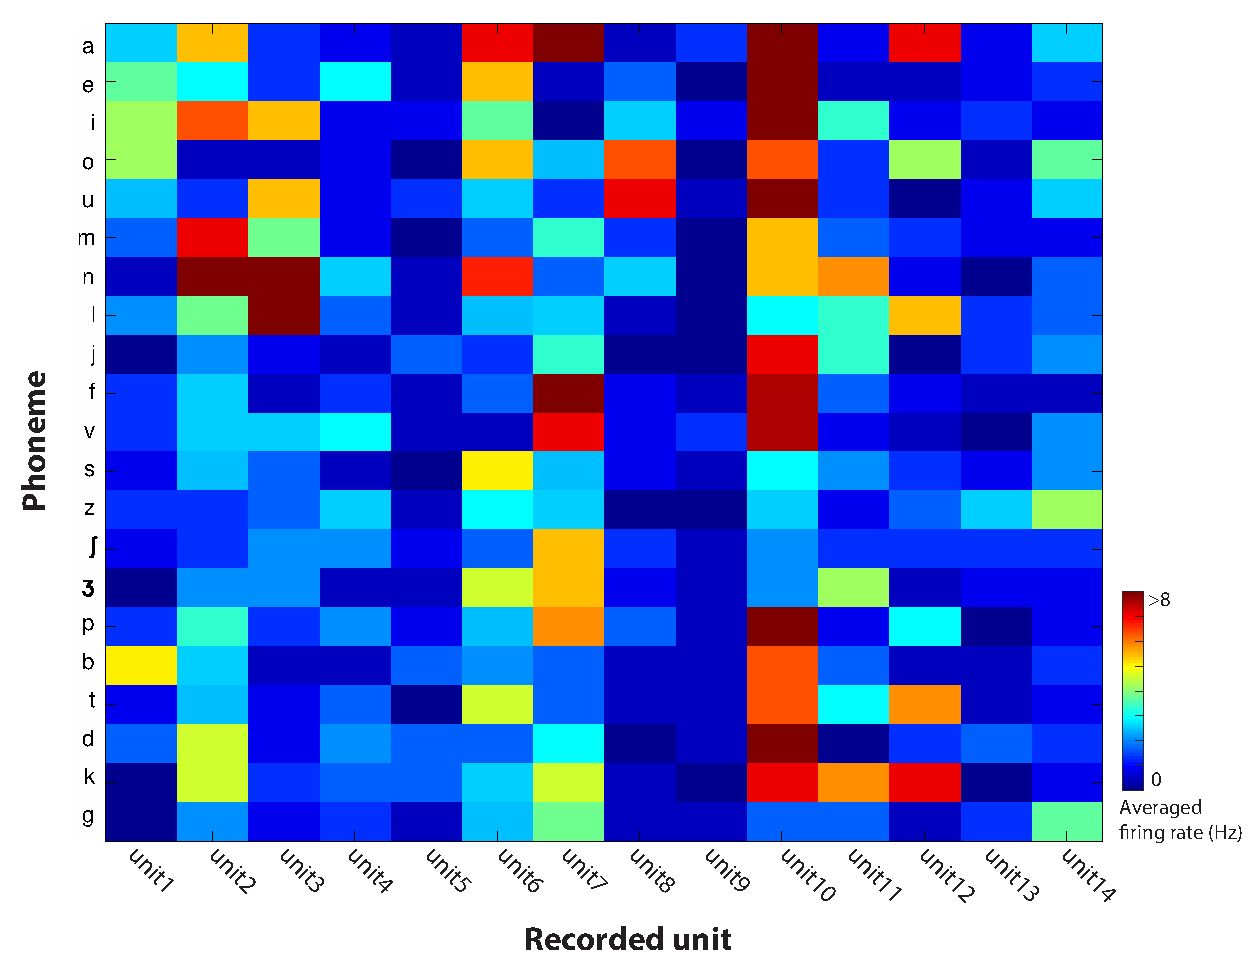
\includegraphics[width=\linewidth]{Figures/Ch3/Figure3_new.eps}
\caption{Neural tuning to phonemes for all units. Color scale represents mean spike-count activity in the optimal time window.}
\end{figure}

\subsection{The functional organization of phonemes}
Figure 3.2 shows that units are mainly selective to subsets of phonemes, and not to specific ones, suggesting that neural representations of phonemes are high-dimensional and distributed, yet, possibly clustered. We therefore further explore the organization of phonemes in activity space. We represent each phoneme in a high-dimensional space, in which dimensions represent mean firing rates in the time bins. Since there are fourteen units and four time bins for each, the resulting space is 48-dimensional. Next, we visualize the neural representations by projecting them into a lower-dimensional space, spanned by the three principal components of the data. Figure 3.3A presents the result. Sonorant phonemes - vowels (/aeiou/) and nasal-approximants(/nmlj/) - are colored in green, obstruents in blue.

\begin{figure}[H]
\vspace{.3in}
\includegraphics[width=\linewidth]{Figures/Ch3/Figure4_new.eps}
\caption{(A) Neural representations of phonemes along the first two principal components of the data. Colors: sonorant phonemes (red), obstruent phonemes (blue); (B) Hierarchical clustering. Top panel depicts a similarity matrix among the neural representations (to enhance color contrasts, diagonal values were manually set to zero). Colors: sonorant phonemes (red), obstruent phonemes (black). Bottom panel depicts hierarchical clustering of neural representations of phonemes based on single-cells recordings in the STG during listening. (C) Confusion among place-of-articulation features of consonants: labial, alveolar, palatal, velar, glottal (chance level - 0.25) (D) confusion matrix among manner-of-articulation features of consonants: plosives, fricatives, nasals, approximants and vowels.}
\end{figure}

Figure 3.3A suggests that sonorant and obstruent phonemes have relatively distinct neural representations. We therefore further experiment with the data in the following way. First, using hierarchical clustering, we test whether additional phonologically defined clusters of phonemes can be identified in activation space. Clusters may indicate about invariances in the neural response to specific groups of phonemes. Figure 3.3B presents the hierarchical clustering of the single-unit responses. A central cluster of obstruents (except for /k/, and including /e/) is observed, separated from most sonorants - the vowels /aoiu/ and nasal-approximants /nmlj/. In addition, the obstruent cluster is further divided into a sub-cluster containing all stridents /s\textipa{S}z\textipa{Z}/. 

\begin{figure}[H]
\vspace{.3in}
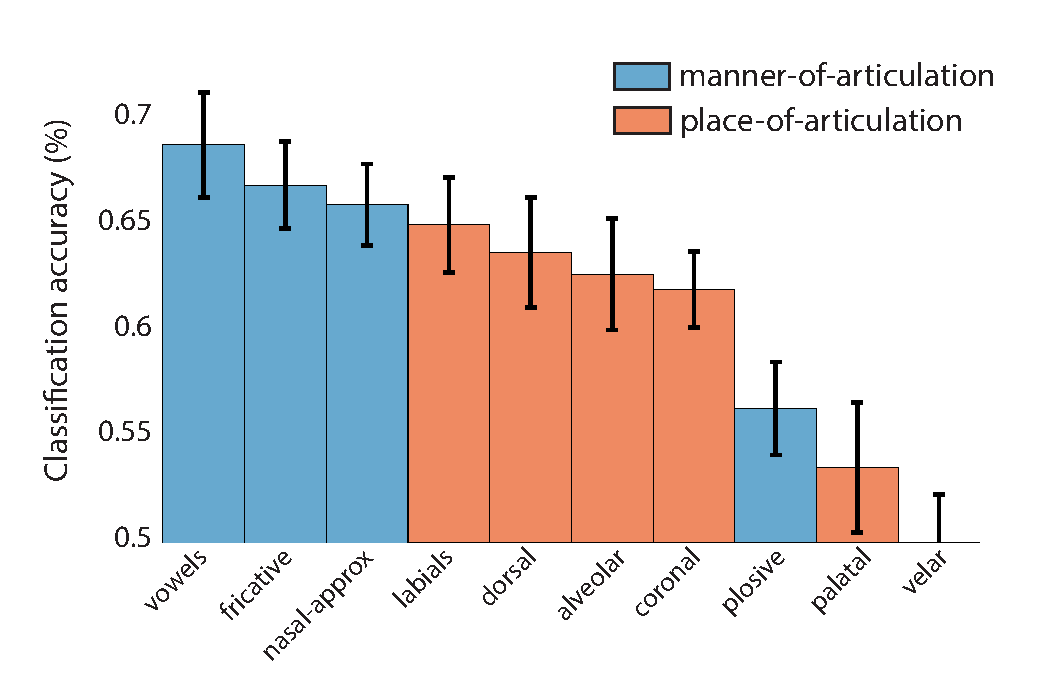
\includegraphics[width=\linewidth]{Figures/Ch3/Figure5_new.eps}
\caption{Phoneme-classification accuracy for each binary feature, e.g., [+nasals] vs. [-nasal], [+labial] vs. [-labial].}
\end{figure}

Figure 3.3B points to a functional organization based on manner-of-articulation features, with distinct clusters for obstruents and sonorants, and clustering of strident phonemes. However, the picture is less pronounced compared to ECoG studies. We therefore quantify and compare the invariance to manner- and place-of-articulation features directly, using probabilistic modelling. We model the spiking-pattern response to phonological features using a Naive-Bayes classifier, assuming the spike generation follows a Poisson process (section 3.2.5). To test invariance to features, we train the model to classify among phonemes grouped according to either manner- or place-of-articulation features. Higher classification performance indicates about higher invariance of the neural response, and classification errors indicate about similarity among phonological features. For both manner- and place-of-articulation, we label the phonemes according to four phonological features. For manner, we label /aeiou/ as 'vowel', /nmlj/ as 'nasal-approximant', /fvszS/ as 'fricative', /bdgptk/ as 'plosives'; and for place-of-articulation, /bpfvm/ as 'labial', /tdszn/ as 'alveolar', /\textipa{S}\textipa{Z}/ as palatal and /kg/ as velar. We train the classifier on a subset of the data and test predictions on a left-out data. Figure 3.3 (Panels C and D) presents the mean posterior distribution for all phonological features, organized in a confusion matrix - color scale indicates probability values. Only values that are significantly ($p-value<0.05$) greater than chance level are presented.

Finally, we further experiment with the data by comparing binary classification across various phonological features. For each phonological feature, e.g. [nasal], we label all phonemes as either [+nasal] or [-nasal]. We then calculate prediction accuracy based on all test trials, by taking the mode of the posterior distribution as the prediction of the model (section 3.2.5). Figure 3.4 presents prediction accuracies for various phonological features. Results are ordered from the highest to the lowest accuracy, highlighting the dominance of manner features.


\subsection{A comparison between neural and behavioral data}
Phoneme similarity in the cognitive system can be estimated from behavioral tasks, assuming the more confusable two phonemes are the more similar they are. We test whether phoneme similarity, as estimated from behavioral tasks, is reflected in the neural activity in the STG. For this, we generate two phoneme-similarity matrices - a behavioral and a neural matrix (section 3.2.6), and calculated the Spearman correlation between the two. We find a moderate correlation between the behavioral and neural similarity matrices ($\rho = 0.45, p-value < 10^{-3}$).


\section{Summary and Discussion}
We recorded neural activity from six patients during a listening task in which vowels and consonant-vowel syllables were aurally presented. We characterized spiking activity from fourteen neurons in the STG that were consistently responsive to the speech stimuli. We inquired into two theoretical questions. The first focused on the functional organization of phonemes in the STG. We tested whether the organization of neural representations of phonemes at the cellular level is dominated by manner-of-articulation features, as was found by previous electroencephalography studies. The second question addressed the relation between cognitive and neural representations of phoneme similarities. Using the same of stimuli as with clinical patients, we derived cognitive phoneme similarities from phoneme-confusability data in healthy subjects. We then compared the perceptual similarities to the similarities derived from population spiking activity in the STG.

To characterize the distributed, yet possibly clustered, response patterns to different phonemes, we explored the recorded spiking activity with several methods. We first represented each phoneme in activity space in which dimensions correspond to spike counts, calculated in the most informative time window found for each unit. We then visualized the structure of phoneme representations by projecting it into a lower dimensional space (Figures 3A). The resulting structure reveals a separate representation of sonorant and obstruent phonemes, as was previously shown at the population level. The sonorant-obstruent distinction can be naturally described by acoustic correlates, but much less with gestural ones, as sonorant and obstruent phonemes have highly varied articulations.   

To further specify relations among phoneme representations, we next examined the hierarchical clustering of the data in activation space. We found that most of the sonorant and obstruent phonemes cluster separately, and that strident fricatives form a sub-cluster of the obstruent one. These results point to a functional organization, which is based on acoustic cues. Sonorants are highly resonant and have identifiable formant structure compared to obstruents. Similarly, stridents have a clear acoustic footprint, characterized by high intensity and high-frequency energy. These results are in accordance with previous ECoG studies, and point to a functional organization that is dominated by manner-of-articulation features. To further quantify this, we next trained a probabilistic classifier, which mimics the generation process of spikes, as recorded by the units. We then compared model predictions when grouping phonemes according to various phonological features. We found that model performance are significantly better when phonemes are grouped according to manner-of-articulation features, compared to place-of-articulation ones (Figures 3C-D \& 4). These results add to the accumulating evidence that neural representations in the STG are dominated by manner-of-articulation.

Finally, we compared the neural and cognitive organizations of phonemes, as estimated from single-cells activity and behavioral data, respectively. Remarkably, spiking activity from the handful of neurons reflects phoneme similarities derived from behavioral results, based on phoneme-confusion experiments using the same set of stimuli. Specifically, the nasal and approximant features show a distinct neural representation with respect to other feature classes, which corresponds to their relatively high perceptual saliency (cite).

Speech signals are composed of continuous streams of high-dimensional acoustic information, which must be encoded in the auditory pathway in a way that ensures robust categorization. The auditory pathway shows an increasing encoding specificity and invariance for speech sounds, from relatively simple acoustic features in early stages, to complex spectrotemporal acoustic patterns in cortical regions. In humans, invariance to phonetic features is thought to be found outside the primary auditory cortex, in STG and STS subregions \citep{Dewitt2012} (in animals, \citealp[see]{mesgarani2008phoneme}). This study provides another layer of evidence, showing that the functional organization of phonemes in the STG, as revealed by population spiking activity, is in accordance to auditory theories and in contrast to gestural theories of speech perception \citep{liberman1985motor, browman1992articulatory}.

%% General Discussion
\lhead{\emph{General Discussion}}
\chapter*{General Discussion and Conclusions}
\addcontentsline{toc}{chapter}{General discussion and conclusions}
A large body of literature in neuropsychology provides varied support to the view that reading errors made by dyslexic people can result from distinct and independent causes \citep{mn73, sw77, c83, c96, shallice2000selective, friedmann2001letter}. Accordingly, dyslexia has been analyzed into subtypes of dyslexia, each corresponds to a different deficit in the process of reading \citep[for a review, see,  ][]{ck12}. These neuropsychological studies have gained further support by research in neuroscience, looking into brain function during reading \citep{fiebach2002fmri, joubert2004neural, levy2009testing}, and were accompanied by computational simulations of the suggested underlying sub-processes \citep{coltheart2001drc, perry2007nested}. This thread of research has been continuously striving to identify new subtypes of dyslexia in order to improve our understanding of the process of reading and to advance therapeutic methods. In particular, recently, a new family of subtypes of dyslexia was identified, which was suggested to originate from phonological-processing deficits in the sublexical route \citep{Gvion2010, Gvion2012}. Throughout this thesis we explored the rich phenomenology of reading from a computational-modelling, data-driven, perspective. 

Alongside the above evidences, a similarly large body of studies subsists in the literature, supporting an opposite view, which describes dyslexia as resulting from a single cause \citep{stanovich1988explaining, s98, s00, ss05, rrddcw03, rs08, d09, bdvsgmg13, vgpsh13, grggvfb02, r14}. These two opposing views were brought together under the term \textit{The dyslexia debate} \citep{eg14}. The first chapter of this thesis provides the first computational study of reading-error patterns, based on the largest existing corpus of reading errors made by dyslexic people. In particular, it directly addresses the dyslexia debate by exploring reading-error patterns with probabilistic graphical models, spelling out the generation process of reading errors in probabilistic terms. This study is the first to provide support to the subtype approach to dyslexia from a computational-modelling point of view. In addition, we suggest the most predictive model, among those we explored, as an easily accessible, cheap and objective diagnosis tool for dyslexia. Although our models were based on error-types, which were manually marked by clinicians, this stage can be automated as well, thus achieving a completely automated screening test. Speech-recognition algorithms have made significant improvement in recent years, and can be efficiently modified for the task of identifying error types such as letter substitution, omission or regularization errors, in both word and nonword reading. With continuously growing databases of reading errors, future research can extend this new line of research, addressing the issue with even larger-scale experiments. Such future study can further benefit both the theoretical and clinical aspects of the field. 

Motivated by recent findings about a new family of dyslexia subtypes that involves specific phonological-processing errors, chapter 2 addresses the question of phoneme similarity from a new computational-modelling perspective. The methodological approach presented in this study enables the quantification of the contribution of each subphonemic feature to perceptual phoneme similarities, in a data-driven manner. Results reveal an order among subphonemic features in English with respect to their perceptual saliency - voicing, nasality, distributed-stridents and approximants. Interestingly, these four leading phoneme groups correspond to observed phoneme-related errors described in reading: voicing, nasality, strident and approximant-substitution errors. Before comparing these, we suggest to first distinguish between substitution errors that can be termed \textit{inter-class} errors, in which a phoneme from one natural class, e.g. [+voice], is substituted with a phoneme from the opposite class [-voice], as when reading 'this' as 'thiz'. Another example of inter-class error is when reading 'near' as 'dear', with respect to nasality. Inter-class errors were reported in dyslegzia with respect to voicing, and in nasalexia with respect to nasality. In contrast, we call \textit{intra-class} errors, errors in which a phoneme is substituted with another phoneme from the same class, as when reading 'sip' as 'ship', with respect to stridency. Intra-class errors were observed for stridents and approximants \citep[unpublished]{friedmann}. In contrast to intra-class errors, voicing and nasality inter-class errors in English seem in variance to the relatively high saliency of these features. One would expect a low rate of inter-class errors for features that are highly discriminatives, since they render the corresponding pair of phonemes less similar and thus less prone to errors. One explanation for this may be that phoneme-related reading errors do not follow perceptual phoneme similarity, but are also influenced by production processes as well - possible articulatory similarities among phonemes can therefore affect error rates in addition to perceptual similarities\footnote{Note that phoneme-related reading errors were localized to the sublexical route, before the phonological output buffer and articularoy system, and are therefore different than mere speech errors \citep{Gvion2010}.}. Pairs of phonemes that are relatively perceptually distinct, such as /n/-/d/, can be articulatorily similar (velum lowering in this case). The role of perceptual and articulatory similarities among phonemes in sublexcial reading, silent or reading aloud, is yet unclear and requires future research. Taken together, the discrepancy between perceptual saliency and error prevalence points to the conclusion that perceptual similarities may not solely account for phoneme-related reading errors in dyslexia. With that said, we would like to point out a relationship between perception and production, proposed by the quantal theory of speech perception which may shed additional light on the question in hand. This theory suggests that languages prefer distinctive features that are optimal in maximizing acoustic dissimilarities while minimizing articulatory effort \citep{stevens1989quantal, stevens2002toward}. Voicing and nasality are therefore optimal in this sense. They have highly discriminative power, as our study shows for English, with relatively minimal articulatory effort (chord vibration and velum lowering, respectively). These features therefore seem liable targets for selective deficits in many languages. Similarly, chapter 2 shows that distributed stridents have relatively high perceptually discriminative power, and have a minimal articulatory difference from non-distributed stridents (alveolar to post-alveolar articulator change). Accordingly, substitution errors such as /g/-/k/ (voicing), /n/-/d/(nasality) and /s/-/\textipa{S}/(distributed-stridency) may be expected to be more frequent and observable, taking into account both perceptual and articulatory similarities.

Chapter 3 further inquires into perceptual phoneme similarity by recording spiking activity from single neurons in the superior temporal gyrus during a phoneme-listening task. Consistently with previous ECoG and EEG studies, our results supports a functional organization of phonemes that is dominated by manner-of-articulation features, as revealed also at the cellular level. We found that neural representations of phonemes cluster according to sonorant and obstruent features, and that manner-of-articulation features are better decoded from spiking-activity data compared to place-of-articulation. These results provide additional support to auditory theories of speech perception \citep{stevens1989quantal, stevens2002toward}, and are in contrast to motor theories \citep{liberman1985motor, browman1992articulatory}. Remarkably, spiking activity from a handful of neurons - fourteen, collected from six patients - reflects phoneme similarities derived from behavioral results, based on phoneme-confusion experiments using the same set of stimuli. Specifically, the nasal and approximant features show distinct neural representations compared to other feature classes, which corresponds to their relatively high perceptual saliency as descirbed in chapter 2. 

Overall, the thesis demonstrates the contribution of data-driven computational modelling to the field of reading disorders and neurolinguistics. Specifically, its main contributions are:


\begin{itemize}
   \item  Study 1
   \begin{itemize}
        \item  Support to the subtype approach to dyslexia from a probabilistic point of view.
        \item Laying the ground for an automatization of the diagnosis process of dyslexia, based on error types.
    \end{itemize}
   
    \item  Study 2
    \begin{itemize}
        \item A new methodological approach to the problem of phoneme similarity.
        \item The first phoneme-confusion dataset for Hebrew.
        \item A quantification of the contribution of phonological features to phoneme similarity.
   \end{itemize}
   
   \item Study 3
   \begin{itemize}
        \item A new dataset of single-cell activity in response to phonemic stimuli.
        \item Characterization of the functional organization of phonemes at the cellular level, and a comparison to the cognitive one as derived from behavioral data.
        \item Support to auditory theories of speech perception.
   \end{itemize}
\end{itemize}


%% ----------------------------------------------------------------
% Now begin the Appendices, including them as separate files

\addtocontents{toc}{\vspace{2em}} % Add a gap in the Contents, for aesthetics

%\appendix % Cue to tell LaTeX that the following 'chapters' are Appendices

%\input{Appendices/AppendixA}	% Appendix Title

%\input{Appendices/AppendixB} % Appendix Title

%\input{Appendices/AppendixC} % Appendix Title

\addtocontents{toc}{\vspace{2em}}  % Add a gap in the Contents, for aesthetics
\backmatter

%% ----------------------------------------------------------------
\label{References}
\lhead{\emph{References}}  % Change the left side page header to "Bibliography"
\bibliography{bib_thesis.bib}  % The references (bibliography) information are stored in the file named 
%\printbibliography


\end{document}  % The End